\documentclass[a4paper,12pt,oneside]{memoir}

\usepackage{postgresql}
\graphicspath{{images/}{schemes/}{software/}}

\usepackage[svgnames]{xcolor}
\ifpdf
  \usepackage{pdfcolmk}
\fi
\ifxetex
  \usepackage{fontspec}
\fi

\DeclareRobustCommand{\cs}[1]{\texttt{\char`\\#1}}
\newlength{\tpheight}\setlength{\tpheight}{0.9\textheight}
\newlength{\txtheight}\setlength{\txtheight}{0.9\tpheight}
\newlength{\tpwidth}\setlength{\tpwidth}{0.9\textwidth}
\newlength{\txtwidth}\setlength{\txtwidth}{0.9\tpwidth}
\newlength{\drop}

\newenvironment{showtitle}{%
  \begin{boxminipage}[c][\tpheight]{\tpwidth}
  \centering\begin{vplace}\begin{minipage}[c][\txtheight]{\txtwidth}}%
{\end{minipage}\end{vplace}\end{boxminipage}}

\definecolor{Dark}{gray}{.2}
\definecolor{MedDark}{gray}{.4}
\definecolor{Medium}{gray}{.6}
\definecolor{Light}{gray}{.8}

\newcommand*{\titleGM}{\begingroup% Gentle Madness
\drop = 0.1\txtheight
\vfill
  \hbox{%
  \hspace*{0.2\txtwidth}%
  \rule{1pt}{\txtheight}
  \hspace*{0.05\txtwidth}%
%\fbox{%
\parbox[b]{0.75\txtwidth}{
  \vbox{%
    \vspace{\drop}
    {\noindent\HUGE\bfseries Работа с Postgresql}\\[2\baselineskip]
    {\Large\itshape настройка, масштабирование}\\[4\baselineskip]
    {\Large Алексей Васильев Юрьевич}\par
    \vspace{0.5\txtheight}
    {\noindent http://leopard.in.ua}\\{\noindent 2011}\\[\baselineskip]
    }% end of vbox
}% end of parbox
%}% end of fbox
  }% end of hbox
\vfill
\endgroup}

\newcommand*{\titleTMB}{\begingroup% Three Men in a Boat
\drop=0.1\textheight
\centering
\settowidth{\unitlength}{\LARGE Работа с Postgresql: настройка, масштабирование}
\vspace*{\baselineskip}
{\large\scshape Васильев А.Ю.}\\[\baselineskip]
\rule{\unitlength}{1.6pt}\vspace*{-\baselineskip}\vspace*{2pt}
\rule{\unitlength}{0.4pt}\\[\baselineskip]
{\LARGE Работа с Postgresql}\\[\baselineskip]
{\itshape настройка, масштабирование}\\[0.2\baselineskip]
\rule{\unitlength}{0.4pt}\vspace*{-\baselineskip}\vspace{3.2pt}
\rule{\unitlength}{1.6pt}\\[\baselineskip]
{\large\scshape справочное пособие}\par
\vfill
{\large\scshape 2011-2013}\\[\baselineskip]
{\small\scshape Creative Commons Attribution-Noncommercial 2.5}\par
\vspace*{\drop}
\endgroup}

% Title Page
\title{Работа с Postgresql: настройка, масштабирование}
\author{Алексей Васильев Юрьевич}


\makepagestyle{myindex}
\makeheadrule{myindex}{\textwidth}{\normalrulethickness}
\makeevenhead{myindex}{\rightmark}{}{\leftmark}
\makeoddhead{myindex}{\rightmark}{}{\leftmark}
\makeevenfoot{myindex}{}{\thepage}{}
\makeoddfoot{myindex}{}{\thepage}{}

\makeevenhead{myindex}{\thepage}{}{\slshape\leftmark}
\makeoddhead{myindex}{\slshape\rightmark}{}{}

\makepsmarks{myindex}{%
\nouppercaseheads
\createmark{chapter}{left}{shownumber}{\@chapapp\ }{. \ }
\createmark{section}{right}{shownumber}{}{. \ }
\createplainmark{toc}{both}{\contentsname}
\createplainmark{lof}{both}{\listfigurename}
\createplainmark{lot}{both}{\listtablename}
\createplainmark{bib}{both}{\bibname}
\createplainmark{index}{both}{\indexname}
\createplainmark{glossary}{both}{\glossaryname}
}

\semiisopage



\begin{document}

\pagestyle{empty}
\titleGM
\clearpage

\thispagestyle{empty}
При написании книги(мануала, или просто шпаргалки) использовались материалы:
\begin{itemize}
\item PostgreSQL: настройка производительности. Алексей Борзов (Sad Spirit) borz\_off@cs.msu.su, \\
http://www.phpclub.ru/detail/store/pdf/postgresql-performance.pdf
\item Настройка репликации в PostgreSQL с помощью системы Slony-I, Eugene Kuzin eugene@kuzin.net, \\
http://www.kuzin.net/work/sloniki-privet.html
\item Установка Londiste в подробностях, Sergey Konoplev gray.ru@gmail.com, \\
http://gray-hemp.blogspot.com/2010/04/londiste.html
\item Учебное руководство по pgpool-II, Dmitry Stasyuk, \\
http://undenied.ru/2009/03/04/uchebnoe-rukovodstvo-po-pgpool-ii/
\item Горизонтальное масштабирование PostgreSQL с помощью PL/Proxy, Чиркин Дима dmitry.chirkin@gmail.com, \\
http://habrahabr.ru/blogs/postgresql/45475/
\item Hadoop, Иван Блинков wordpress@insight-it.ru, \\
http://www.insight-it.ru/masshtabiruemost/hadoop/
\item Up and Running with HadoopDB, Padraig O'Sullivan, \\
http://posulliv.github.com/2010/05/10/hadoopdb-mysql.html
\item Масштабирование PostgreSQL: готовые решения от Skype, Иван Золотухин, \\
http://postgresmen.ru/articles/view/25
\item Streaming Replication, \\
http://wiki.postgresql.org/wiki/Streaming\_Replication
\item Шардинг, партиционирование, репликация - зачем и когда?, Den Golotyuk, \\
http://highload.com.ua/index.php/2009/05/06/шардинг-партиционирование-репликац/
\end{itemize}


\clearpage

\setcounter{page}{3}
\pagestyle{myindex}
%\chapterstyle{bianchi}
\chapterstyle{ell}
%\chapterstyle{ger}
%\chapterstyle{madsen}
%\chapterstyle{veelo}
\setcounter{tocdepth}{2}% subsections and above
\tableofcontents

\chapter{Введение}
\begin{epigraphs}
\qitem{Послушайте~--- и Вы забудете, посмотрите~--- и Вы запомните, сделайте~--- и Вы поймете.}{Конфуций}
\end{epigraphs}

Данная книга не дает ответы на все вопросы по работе с PostgreSQL. 
Главное её задание~--- показать возможности PostgreSQL, методики 
настройки и масштабируемости этой СУБД. 
В любом случае, выбор метода решения поставленной задачи остается за разработчиком или администратором СУБД. 
%performance begin
\chapter{Настройка производительности}
\begin{epigraphs}
\qitem{Теперь я знаю тысячу способов, как не нужно делать лампу накаливания.}{Томас Алва Эдисон}
\end{epigraphs}
\section{Введение}
Скорость работы, вообще говоря, не является основной причиной использования реляционных СУБД. 
Более того, первые реляционные базы работали медленнее своих предшественников. 
Выбор этой технологии был вызван скорее
\begin{itemize}
\item возможностью возложить поддержку целостности данных на СУБД;
\item независимостью логической структуры данных от физической.
\end{itemize}

Эти особенности позволяют сильно упростить написание приложений, но требуют для 
своей реализации дополнительных ресурсов.

Таким образом, прежде, чем искать ответ на вопрос <<как заставить РСУБД работать быстрее в моей задаче?>> 
следует ответить на вопрос <<нет ли более подходящего средства для решения моей задачи, чем РСУБД?>> 
Иногда использование другого средства потребует меньше усилий, чем настройка производительности.

Данная глава посвящена возможностям повышения производительности PostgreSQL. 
Глава не претендует на исчерпывающее изложение вопроса, наиболее полным и точным руководством по 
использованию PostgreSQL является, конечно, официальная документация и официальный FAQ. 
Также существует англоязычный список рассылки postgresql-performance, посвящённый именно этим вопросам.
Глава состоит из двух разделов, первый из которых ориентирован скорее на администратора, 
второй~--- на разработчика приложений. Рекомендуется прочесть оба раздела: отнесение многих вопросов к 
какому-то одному из них весьма условно.

\subsection{Не используйте настройки по умолчанию}
По умолчанию PostgreSQL сконфигурирован таким образом, чтобы он мог быть запущен практически 
на любом компьютере и не слишком мешал при этом работе других приложений. Это особенно касается используемой памяти. 
Настройки по умолчанию подходят только для следующего использования:
с ними вы сможете проверить, работает ли установка PostgreSQL, создать тестовую базу 
уровня записной книжки и потренироваться писать к ней запросы.
Если вы собираетесь разрабатывать (а тем более запускать в работу) реальные 
приложения, то настройки придётся радикально изменить.
В дистрибутиве PostgreSQL, к сожалению, не поставляется файлов с <<рекомендуемыми>> настройками. 
Вообще говоря, такие файлы создать весьма сложно, т.к. оптимальные настройки конкретной 
установки PostgreSQL будут определяться:
\begin{itemize}
\item конфигурацией компьютера;
\item объёмом и типом данных, хранящихся в базе;
\item отношением числа запросов на чтение и на запись;
\item тем, запущены ли другие требовательные к ресурсам процессы (например, вебсервер).
\end{itemize}

\subsection{Используйте актуальную версию сервера}
Если у вас стоит устаревшая версия PostgreSQL, то наибольшего ускорения работы вы сможете 
добиться, обновив её до текущей. Укажем лишь наиболее значительные из связанных с производительностью изменений.
\begin{itemize}
\item В версии 7.1 появился журнал транзакций, до того данные в таблицу сбрасывались каждый раз при успешном завершении транзакции.
\item В версии 7.2 появились:
\begin{itemize}
\item новая версия команды VACUUM, не требующая блокировки;
\item команда ANALYZE, строящая гистограмму распределения данных в столбцах, что позволяет выбирать более 
быстрые планы выполнения запросов;
\item подсистема сбора статистики.
\end{itemize}
\item В версии 7.4 была ускорена работа многих сложных запросов (включая печально известные подзапросы IN/NOT IN).
\item В версии 8.0 были внедрены метки востановления, улучшение управления буфером, CHECKPOINT и VACUUM улучшены.
\item В версии 8.1 был улучшен одновременный доступ к разделяемой памяти, автоматически использование индексов для MIN() и MAX(),
pg\_autovacuum внедрен в сервер (автоматизирован), повышение производительности для секционированных таблиц.
\item В версии 8.2 была улучшена скорость множества SQL запросов, усовершенствован сам язык запросов. 
\item В версии 8.3 внедрен полнотекстовый поиск, поддержка SQL/XML стандарта, параметры конфигурации сервера могут быть 
установлены на основе отдельных функций.
\item В версии 8.4 было внедрено общие табличные выражения, рекурсивные запросы, параллельное восстановление, улучшенна 
производительность для EXISTS/NOT EXISTS запросов.
\item В версии 9.0 <<репликация из коробки>>, VACUUM/VACUUM FULL стали быстрее, расширены хранимые процедуры.
\end{itemize}
Следует также отметить, что большая часть изложенного в статье материала относится к версии сервера не ниже 8.4.

\subsection{Стоит ли доверять тестам производительности}
Перед тем, как заниматься настройкой сервера, вполне естественно ознакомиться с опубликованными данными по 
производительности, в том числе в сравнении с другими СУБД. К сожалению, многие тесты служат не столько для 
облегчения вашего выбора, сколько для продвижения конкретных продуктов в качестве <<самых быстрых>>.
При изучении опубликованных тестов в первую очередь обратите внимание, соответствует ли величина и тип 
нагрузки, объём данных и сложность запросов в тесте тому, что вы собираетесь делать с базой? Пусть, например, 
обычное использование вашего приложения подразумевает несколько одновременно работающих 
запросов на обновление к таблице в миллионы записей. В этом случае СУБД, которая в несколько раз 
быстрее всех остальных ищет запись в таблице в тысячу записей, может оказаться не лучшим выбором.
Ну и наконец, вещи, которые должны сразу насторожить:
\begin{itemize}
\item Тестирование устаревшей версии СУБД.
\item Использование настроек по умолчанию (или отсутствие информации о настройках).
\item Тестирование в однопользовательском режиме (если, конечно, вы не предполагаете использовать СУБД именно так).
\item Использование расширенных возможностей одной СУБД при игнорировании расширенных возможностей другой.
\item  Использование заведомо медленно работающих запросов (см. пункт 3.4).
\end{itemize}


\section{Настройка сервера}
В этом разделе описаны рекомендуемые значения параметров, влияющих на производительность СУБД. Эти параметры 
обычно устанавливаются в конфигурационном файле postgresql.conf и влияют на все базы в текущей установке.


\subsection{Используемая память}
\subsubsection{Общий буфер сервера: shared\_buffers}
PostgreSQL не читает данные напрямую с диска и не пишет их сразу на диск. Данные загружаются в общий буфер сервера, 
находящийся в разделяемой памяти, серверные процессы читают и пишут блоки в этом буфере, а затем уже 
изменения сбрасываются на диск. 

Если процессу нужен доступ к таблице, то он сначала ищет нужные блоки в 
общем буфере. Если блоки присутствуют, то он может продолжать работу, если нет~--- делается системный вызов для 
их загрузки. Загружаться блоки могут как из файлового кэша ОС, так и с диска, и эта операция может оказаться весьма <<дорогой>>.

Если объём буфера недостаточен для хранения часто используемых рабочих данных, то они будут постоянно 
писаться и читаться из кэша ОС или с диска, что крайне отрицательно скажется на производительности.

В то же время не следует устанавливать это значение слишком большим:
это НЕ вся память, которая нужна для работы PostgreSQL, это только размер разделяемой между процессами PostgreSQL памяти, 
которая нужна для выполнения активных операций. Она должна занимать меньшую часть оперативной памяти вашего компьютера, так как 
PostgreSQL полагается на то, что операционная система кэширует файлы, и не 
старается дублировать эту работу. Кроме того, чем больше памяти будет отдано под буфер, тем 
меньше останется операционной системе и другим приложениям, что может привести к своппингу.

К сожалению, чтобы знать точное число shared\_buffers, нужно 
учесть количество оперативной памяти компьютера, размер базы данных, число соединений и сложность запросов, так что лучше 
воспользуемся несколькими простыми правилами настройки.

На выделенных серверах полезным объемом будет значение от 8 МБ до 2 ГБ. 
Объем может быть выше, если у вас большие активные порции базы данных, сложные запросы, большое число 
одновременных соединений, длительные транзакции, вам доступен большой объем оперативной памяти или большее количество 
процессоров. И, конечно же, не забываем об остальных приложениях. Выделив слишком много памяти для базы данных, 
мы можем получить ухудшение производительности. 
В качестве начальных значений можете попробовать следующие:
\begin{itemize}
\item Начните с 4 МБ (512) для рабочей станции
\item Средний объём данных и 256--512 МБ доступной памяти: 16--32 МБ (2048--4096)
\item Большой объём данных и 1--4 ГБ доступной памяти: 64--256 МБ (8192--32768)
\end{itemize}

Для тонкой настройки параметра установите для него большое значение и потестируйте базу при обычной нагрузке. 
Проверяйте использование разделяемой памяти при помощи ipcs или других утилит. Рекомендуемое значение параметра 
будет примерно в 1,2~--2 раза больше, чем максимум использованной памяти. Обратите внимание, что память под буфер 
выделятся при запуске сервера, и её объём при работе не изменяется. Учтите также, что настройки ядра операционной 
системы могут не дать вам выделить большой объём памяти. В руководстве администратора PostgreSQL описано, как 
можно изменить эти настройки: http://developer.postgresql.org/docs/postgres/kernel-resources.html

Вот несколько примеров, полученных на личном опыте и при тестировании:
\begin{itemize}
\item Laptop, Celeron processor, 384 МБ RAM, база данных 25 МБ: 12 МБ
\item Athlon server, 1 ГБ RAM, база данных поддержки принятия решений 10 ГБ: 200 МБ
\item Quad PIII server, 4 ГБ RAM, 40 ГБ, 150 соединений, <<тяжелые>> транзакции: 1 ГБ
\item Quad Xeon server, 8 ГБ RAM, 200 ГБ, 300 соединений, <<тяжелые>> транзакции: 2 ГБ
\end{itemize}

\subsubsection{Память для сортировки результата запроса: work\_mem}
Ранее известное как sort\_mem, было переименовано, так как сейчас определяет максимальное количество оперативной памяти, 
которое может выделить одна операция сортировки, агрегации и др. Это не разделяемая память, work\_mem выделяется отдельно 
на каждую операцию (от одного до нескольких раз за один запрос). Разумное значение параметра определяется следующим образом: 
количество доступной оперативной памяти (после того, как из общего объема вычли память, требуемую для других приложений, и 
shared\_buffers) делится на максимальное число одновременных запросов умноженное на среднее число операций в запросе, которые 
требуют памяти.

Если объём памяти недостаточен для сортироки некоторого результата, то серверный процесс будет использовать 
временные файлы. Если же объём памяти слишком велик, то это может привести к своппингу.

Объём памяти задаётся параметром work\_mem в файле postgresql.conf. Единица измерения параметра~--- 1 кБ. 
Значение по умолчанию~--- 1024. В качестве начального значения для параметра можете взять 2--4\% доступной памяти.
Для веб-приложений обычно устанавливают низкие значения work\_mem, так как запросов обычно много, но они простые, обычно хватает 
от 512 до 2048 КБ. С другой стороны, приложения для поддержки принятия решений с сотнями строк в каждом запросе и десятками 
миллионов столбцов  в таблицах фактов часто требуют work\_mem порядка 500 МБ. Для баз данных, которые используются и так, и так, 
этот параметр можно устанавливать для каждого запроса индивидуально, используя настройки сессии. Например, 
при памяти 1--4 ГБ рекомендуется устанавливать 32--128 MB. 

\subsubsection{Память для работы команды VACUUM: maintenance\_work\_mem}
Предыдущее название в PostgreSQL 7.x vacuum\_mem. Этот параметр задаёт объём памяти, используемый командами 
VACUUM, ANALYZE, CREATE INDEX, и добавления внешних ключей. 
Чтобы операции выполнялись максимально быстро, нужно устанавливать этот параметр тем выше, чем больше размер таблиц в 
вашей базе данных. Неплохо бы устанавливать его значение от 50 до 75\% размера вашей самой большой таблицы или индекса или, 
если точно определить невозможно, от 32 до 256 МБ. Следует устанавливать большее значение, чем для work\_mem. 
Слишком большие значения приведут к использованию свопа. Например, при памяти 1--4 ГБ рекомендуется устанавливать 128--512 MB.

\subsubsection{Free Space Map: как избавиться от VACUUM FULL}
Особенностями версионных движков БД (к которым относится и используемый в PostgreSQL) является следующее:
\begin{itemize}
\item Транзакции, изменяющие данные в таблице, не блокируют транзакции, читающие из неё данные, и наоборот (это хорошо);
\item При изменении данных в таблице (командами UPDATE или DELETE) накапливается мусор\footnote{под которым понимаются 
старые версии изменённых/удалённых записей} (а это плохо).
\end{itemize}
В каждой СУБД сборка мусора реализована особым образом, в PostgreSQL для этой цели применяется команда VACUUM (описана в пункте 3.1.1).

До версии 7.2 команда VACUUM полностью блокировала таблицу. Начиная с версии 7.2, команда VACUUM накладывает более слабую 
блокировку, позволяющую параллельно выполнять команды SELECT, INSERT, UPDATE и DELETE над обрабатываемой таблицей. 
Старый вариант команды называется теперь VACUUM FULL.

Новый вариант команды не пытается удалить все старые версии записей и, соответственно, уменьшить размер файла, содержащего таблицу, 
а лишь помечает занимаемое ими место как свободное. Для информации о свободном месте есть следующие настройки:
\begin{itemize}
\item \textbf{max\_fsm\_relations}

Максимальное количество таблиц, для которых будет отслеживаться свободное место в общей карте свободного пространства. 
Эти данные собираются VACUUM. Параметр max\_fsm\_relations должен быть не меньше общего количества таблиц во всех 
базах данной установки (лучше с запасом). 

\item \textbf{max\_fsm\_pages}

Данный параметр определяет размер реестра, в котором хранится информация о частично освобождённых страницах данных, 
готовых к заполнению новыми данными. Значение этого параметра нужно установить чуть больше, чем полное число страниц, 
которые могут быть затронуты 
операциями обновления или удаления между выполнением VACUUM. Чтобы определить это число, можно запустить VACUUM VERBOSE ANALYZE 
и выяснить общее число страниц, используемых базой данных. max\_fsm\_pages обычно требует немного памяти, так что на этом 
параметре лучше не экономить. 
\end{itemize}

Если эти параметры установленны верно и информация обо всех изменениях помещается в FSM, 
то команды VACUUM будет достаточно для сборки мусора, если нет~-- понадобится
VACUUM FULL, во время работы которой нормальное использование БД сильно затруднено.

\subsubsection{Прочие настройки}
\begin{itemize}
\item \textbf{temp\_buffers}

Буфер под временные объекты, в основном для временных таблиц.
Можно установить порядка 16 МБ.

\item \textbf{max\_prepared\_transactions}

Количество одновременно подготавливаемых транзакций (PREPARE TRANSACTION).
Можно оставить по дефолту~--- 5.

\item \textbf{vacuum\_cost\_delay} 

Если у вас большие таблицы, и производится много одновременных операций записи, 
вам может пригодиться функция, которая уменьшает затраты на I/O для VACUUM, растягиваяя его по времени. 
Чтобы включить эту функциональность, нужно поднять 
значение vacuum\_cost\_delay выше 0. Используйте разумную задержку от 50 до 200 мс. Для более тонкой настройки повышайте 
vacuum\_cost\_page\_hit и понижайте vacuum\_cost\_page\_limit. Это ослабит влияние VACUUM, увеличив время его выполнения. 
В тестах с параллельными транзакциями Ян Вик (Jan Wieck) получил, что при значениях delay~--- 200, page\_hit~--- 6 и предел~--- 
100 вляние VACUUM уменьшилось более чем на 80\%, но его длительность увеличилась втрое. 

\item \textbf{max\_stack\_depth}

Специальный стек для сервера, в идеале он должен совпадать с размером стека, выставленном в ядре ОС. 
Установка большего значения, чем в ядре, может привести к ошибкам.
Рекомендуется устанавливать 2--4 MB.

\item \textbf{max\_files\_per\_process}

Максимальное количество файлов, открываемых процессом и его подпроцессами в один момент времени.
Уменьшите данный параметр, если в процессе работы наблюдается сообщение <<Too many open files>>.
\end{itemize}


\subsection{Журнал транзакций и контрольные точки}
Журнал транзакций PostgreSQL работает следующим образом: все изменения в файлах данных (в которых находятся таблицы и 
индексы) производятся только после того, как они были занесены в журнал транзакций, при этом записи в журнале должны 
быть гарантированно записаны на диск.

В этом случае нет необходимости сбрасывать на диск изменения данных при каждом успешном завершении транзакции: 
в случае сбоя БД может быть восстановлена по записям в журнале. Таким образом, данные из буферов сбрасываются на диск 
при проходе контрольной точки: либо при заполнении нескольких (параметр checkpoint\_segments, по умолчанию 3) сегментов
журнала транзакций, либо через определённый интервал времени (параметр checkpoint\_timeout, измеряется в секундах, по умолчанию 300).

Изменение этих параметров прямо не повлияет на скорость чтения, но может принести большую пользу, если данные в базе активно изменяются.

\subsubsection{Уменьшение количества контрольных точек: checkpoint\_segments}
Если в базу заносятся большие объёмы данных, то контрольные точки могут происходить слишком часто\footnote{<<слишком часто>> 
можно определить как <<чаще раза в минуту>>. Вы также можете задать параметр checkpoint\_warning (в секундах): 
в журнал сервера будут писаться предупреждения, если контрольные точки происходят чаще заданного.}. 
При этом производительность упадёт из-за постоянного сбрасывания на диск данных из буфера.

Для увеличения интервала между контрольными точками нужно увеличить количество сегментов журнала транзакций (checkpoint\_segments). 
Данный параметр определяет количество сегментов (каждый по 16 МБ) лога транзакций между контрольными точками. 
Этот параметр не имеет особого значения для базы данных, предназначенной преимущественно для чтения, но для баз данных со 
множеством транзакций увеличение этого параметра может оказаться жизненно необходимым. В зависимости от объема данных 
установите этот параметр в диапазоне от 12 до 256 сегментов и, если в логе появляются предупреждения (warning) о том, что 
контрольные точки происходят слишком часто, постепенно увеличивайте его. Место, требуемое на диске, вычисляется по формуле 
(checkpoint\_segments * 2 + 1) * 16 МБ, так что убедитесь, что у вас достаточно свободного места. Например, если вы выставите 
значение 32, вам потребуется больше 1 ГБ дискового пространства.

Следует также отметить, что чем больше интервал между контрольными точками, тем дольше будут восстанавливаться данные по 
журналу транзакций после сбоя.

\subsubsection{fsync и стоит ли его трогать}
Наиболее радикальное из возможных решений~--- выставить значение <<off>> параметру fsync. При этом записи в журнале транзакций не 
будут принудительно сбрасываться на диск, что даст большой прирост скорости записи. Учтите: вы жертвуете надёжностью, в случае 
сбоя целостность базы будет нарушена, и её придётся восстанавливать из резервной копии!

Использовать этот параметр рекомендуется лишь в том случае, если вы всецело доверяете своему <<железу>> и своему источнику 
бесперебойного питания. Ну или если данные в базе не представляют для вас особой ценности.

\subsubsection{Прочие настройки}
\begin{itemize}
\item 
\textbf{commit\_delay} (в микросекундах, 0 по умолчанию) и \textbf{commit\_sib\-lings} (5 по умолчанию) 

определяют задержку между попаданием записи в буфер журнала транзакций и сбросом её на диск. 
Если при успешном завершении транзакции активно не менее commit\_siblings транзакций, то запись будет задержана на время 
commit\_delay. Если за это время завершится другая транзакция, то их изменения будут сброшены на диск вместе, при помощи 
одного системного вызова. Эти параметры позволят ускорить работу, если параллельно выполняется много <<мелких>> транзакций.

\item \textbf{wal\_sync\_method}

Метод, который используется для принудительной записи данных на диск.
Если fsync=off, то этот параметр не используется.
Возможные значения:
\begin{itemize}
\item open\_datasync~--- запись данных методом open() с параметром O\_DSYNC
\item fdatasync~--- вызов метода fdatasync() после каждого commit
\item fsync\_writethrough~--- вызывать fsync() после каждого commit игнорирую паралельные процессы
\item fsync~--- вызов fsync() после каждого commit
\item open\_sync~--- запись данных методом open() с параметром O\_SYNC
\end{itemize}

Не все методы доступны на определенных платформах. По умолчанию устанавливается первый, который доступен в системе.

\item \textbf{full\_page\_writes}

Установите данный параметр в off, если fsync=off. Иначе, когда этот параметр on, PostgreSQL записывает содержимое 
каждой страницы в журнал транзакций во время первой модификации таблицы после контрольной точки. Это необходимо потому 
что страницы могут записаться лишь частично если в ходе процесса ОС "упала". Это приволит к тому, что на диске оказаываются 
новые данные смешанные со старыми. Строкового уровня записи в журнал транзакций может быть не достаточно, что бы полность 
восстановить данные после "падения". full\_page\_writes гарантирует корректное восстановление, ценой увелечения записываемых 
данных в журнал транзакций.(Потому что журнал транзакций все время начинается с контрольной точки. Единственный способ 
снижения объема записи заключается в увеличении checkpoint\_interval).

\item \textbf{wal\_buffers}

Количество памяти используемое в SHARED MEMORY для ведения транзакционных логов\footnote{буфер находится в 
разделяемой памяти и является общим для всех процессов}.
Стоит увеличить буфер до 256--512 кБ, что позволит лучше работать с большими транзакциями.
Например, при доступной памяти 1--4 ГБ рекомендуется устанавливать 256--1024 КБ.

\end{itemize}


\subsection{Планировщик запросов}
Следующие настройки помогают планировщику запросов правильно оценивать стоимости различных 
операций и выбирать оптимальный план выполнения запроса. Существуют 2 глобальные настройки планировщика, 
на которые стоит обратить внимание:
\begin{itemize}
\item \textbf{effective\_cache\_size}

Этот параметр сообщает PostgreSQL примерный объём файлового кэша операционной системы, оптимизатор использует эту оценку для 
построения плана запроса\footnote{Указывает планировщику на размер самого большого объекта в базе данных, который 
теоретически может быть закеширован}.

Пусть в вашем компьютере 1,5 ГБ памяти, параметр shared\_buffers установлен в 32 МБ, а параметр effective\_cache\_size в 800 МБ. 
Если запросу нужно 700 МБ данных, то PostgreSQL оценит, что все нужные данные уже есть в памяти и выберет более агрессивный план с 
использованием индексов и merge joins. Но если effective\_cache\_size будет всего 200 МБ, то оптимизатор вполне может выбрать более 
эффективный для дисковой системы план, включающий полный просмотр таблицы.

На выделенном сервере имеет смысл выставлять effective\_cache\_size в 2/3 от всей оперативной памяти; на сервере с 
другими приложениями сначала нужно вычесть из всего объема RAM размер дискового кэша ОС и память, 
занятую остальными процессами.

\item \textbf{random\_page\_cost} 

Переменная, указывающая на условную стоимость индексного доступа к страницам данных. На серверах с быстрыми дисковыми 
массивами имеет смысл уменьшать изначальную настройку до 3.0, 2.5 или даже до 2.0. Если же активная часть вашей базы данных 
много больше размеров оперативной памяти, попробуйте поднять значение параметра. Можно подойти к выбору оптимального значения 
и со стороны производительности запросов. Если планировщик запросов чаще, чем необходимо, предпочитает последовательные просмотры 
(sequential scans) просмотрам с использованием индекса (index scans), понижайте значение. И наоборот, если планировщик выбирает 
просмотр по медленному индексу, когда не должен этого делать, настройку имеет смысл увеличить. После изменения тщательно тестируйте 
результаты на максимально широком наборе запросов. Никогда не опускайте значение random\_page\_cost ниже 2.0; если вам кажется, 
что random\_page\_cost нужно еще понижать, разумнее в этом случае менять настройки статистики планировщика. 
\end{itemize}

\subsection{Сбор статистики}
У PostgreSQL также есть специальная подсистема~--- сборщик статистики,~--- которая в реальном времени собирает данные об 
активности сервера. Эта подсистема контролируется следующими параметрами, принимающими значения true/false:
\begin{itemize}
\item \textbf{default\_statistics\_target} задаёт объём по умолчанию статистики, собираемой командой ANALYZE (см. пункт 3.1.2). 
Увеличение параметра заставит эту команду работать дольше, но может позволить оптимизатору строить более быстрые планы, 
используя полученные дополнительные данные. Объём статистики для конкретного поля может быть задан командой 
ALTER TABLE \dots SET STATISTICS.
\item \textbf{stats\_start\_collector} включать ли сбор статистики. По умолчанию включён, отключайте, только если статистика вас 
совершенно не интересует.
\item \textbf{stats\_reset\_on\_server\_start} обнулять ли статистику при перезапуске сервера. По умолчанию~--- обнулять.
\item \textbf{stats\_command\_string} передавать ли сборщику статистики информацию о текущей выполняемой команде и времени 
начала её выполнения. По умолчанию эта возможность отключена. Следует отметить, что эта информация будет доступна только 
привилегированным пользователям и пользователям, от лица которых запущены команды, так что проблем с безопасностью быть не должно.
\item \textbf{stats\_row\_level}, \textbf{stats\_block\_level} собирать ли информацию об активности на уровне записей и 
блоков соответственно. По умолчанию сбор отключён.
\end{itemize}

Данные, полученные сборщиком статистики, доступны через специальные системные представления. При установках по умолчанию собирается 
очень мало информации, рекомендуется включить все возможности: дополнительная нагрузка будет невелика, в то время как полученные 
данные позволят оптимизировать использование индексов.
\section{Диски и файловые системы}
Очевидно, что от качественной дисковой подсистемы в сервере БД зависит немалая часть производительности. Вопросы выбора и 
тонкой настройки <<железа>>, впрочем, не являются темой данной статьи, ограничимся уровнем файловой системы.

Единого мнения насчёт наиболее подходящей для PostgreSQL файловой системы нет, поэтому рекомендуется использовать ту, которая лучше 
всего поддерживается вашей операционной системой. При этом учтите, что современные журналирующие файловые системы не намного 
медленнее нежурналирующих, а выигрыш~--- быстрое восстановление после сбоев~--- от их использования велик.

Вы легко можете получить выигрыш в производительности без побочных эффектов, если примонтируете файловую систему, 
содержащую базу данных, с параметром noatime\footnote{при этом не будет отслеживаться время последнего доступа к файлу}.

\subsection{Перенос журнала транзакций на отдельный диск}
При доступе к диску изрядное время занимает не только собственно чтение данных, но и перемещение магнитной головки.

Если в вашем сервере есть несколько физических дисков\footnote{несколько логических разделов на одном диске здесь, 
очевидно, не помогут: головка всё равно будет одна}, то вы можете разнести файлы базы данных и журнал транзакций по разным 
дискам. Данные в сегменты журнала пишутся последовательно, более того, записи в журнале транзакций сразу сбрасываются на диск, 
поэтому в случае нахождения его на отдельном диске магнитная головка не будет лишний раз двигаться, что позволит ускорить запись.

Порядок действий:
\begin{itemize}
\item Остановите сервер (!).
\item Перенесите каталоги pg\_clog и pg\_xlog, находящийся в каталоге с базами данных, на другой диск. 
\item Создайте на старом месте символическую ссылку.
\item Запустите сервер.
\end{itemize}

Примерно таким же образом можно перенести и часть файлов, содержащих таблицы и индексы, на другой диск, но здесь 
потребуется больше кропотливой ручной работы, а при внесении изменений в схему базы процедуру, возможно, придётся повторить.
\section{Примеры настроек}

\subsection{Среднестатистическая настройка для максимальной производительности}

Возможно для конкретного случаю лучше подойдут другие настройки. Внимательно изучите данное руководство и настройте 
PostgreSQL операясь на эту информацию.

RAM~--- размер памяти;
\begin{itemize}
\item shared\_buffers = 1/8 RAM или больше (но не более 1/4);
\item work\_mem в 1/20 RAM;
\item maintenance\_work\_mem в 1/4 RAM;
\item max\_fsm\_relations в планируемое кол--во таблиц в базах * 1.5;
\item max\_fsm\_pages в max\_fsm\_relations * 2000;
\item fsync = true;
\item wal\_sync\_method = fdatasync;
\item commit\_delay = от 10 до 100 ;
\item commit\_siblings = от 5 до 10;
\item effective\_cache\_size = 0.9 от значения cached, которое показывает free;
\item random\_page\_cost = 2 для быстрых cpu, 4 для медленных;
\item cpu\_tuple\_cost = 0.001 для быстрых cpu, 0.01 для медленных;
\item cpu\_index\_tuple\_cost = 0.0005 для быстрых cpu, 0.005 для медленных;
\item autovacuum = on;
\item autovacuum\_vacuum\_threshold = 1800;
\item autovacuum\_analyze\_threshold = 900;
\end{itemize}

\subsection{Среднестатистическая настройка для оконного приложения (1С), 2 ГБ памяти}

\begin{itemize}
\item maintenance\_work\_mem = 128MB
\item effective\_cache\_size = 512MB
\item work\_mem = 640kB
\item wal\_buffers = 1536kB
\item shared\_buffers = 128MB
\item max\_connections = 500
\end{itemize}

\subsection{Среднестатистическая настройка для Web приложения, 2 ГБ памяти}

\begin{itemize}
\item maintenance\_work\_mem = 128MB;
\item checkpoint\_completion\_target = 0.7
\item effective\_cache\_size = 1536MB
\item work\_mem = 4MB
\item wal\_buffers = 4MB
\item checkpoint\_segments = 8
\item shared\_buffers = 512MB
\item max\_connections = 500
\end{itemize}

\subsection{Среднестатистическая настройка для Web приложения, 8 ГБ памяти}

\begin{itemize}
\item maintenance\_work\_mem = 512MB
\item checkpoint\_completion\_target = 0.7
\item effective\_cache\_size = 6GB
\item work\_mem = 16MB
\item wal\_buffers = 4MB
\item checkpoint\_segments = 8
\item shared\_buffers = 2GB
\item max\_connections = 500
\end{itemize}

\section{Автоматическое создание оптимальных настроек: pgtune}

Для оптимизации настроек для PostgreSQL Gregory Smith создал утилиту pgtune\footnote{http://pgtune.projects.postgresql.org/} 
в расчете на обеспечение максимальной производительности для заданной аппаратной конфигурации.
Утилита проста в использовании и в многих Linux системах может идти в составе пакетов. 
Если же нет, можно просто скачать архив и распаковать.
Для начала:
\begin{verbatim}
pgtune -i $PGDATA/postgresql.conf \
-o $PGDATA/postgresql.conf.pgtune
\end{verbatim}
опцией 
\begin{verbatim}-i, --input-config\end{verbatim} 
указываем текущий файл postgresql.conf, 
а 
\begin{verbatim}-o, --output-config\end{verbatim}
указываем имя файла для нового postgresql.conf.

Есть также дополнительные опции для настройки конфига. 
\begin{itemize}
\item 
\begin{verbatim}-M, --memory\end{verbatim}
Используйте этот параметр, чтобы определить общий объем системной памяти. 
Если не указано, pgtune будет пытаться использовать текущий объем системной памяти.

\item 
\begin{verbatim}-T, --type\end{verbatim}
Указывает тип базы данных. Опции: DW,  OLTP,  Web, Mixed, Desktop.

\item 
\begin{verbatim}-c, --connections\end{verbatim}
Указывает максимальное количество соединений. Если он не указан, это будет братся взависимости от типа базы данных.

\end{itemize}

Хочется сразу добавить, что pgtune не панацея для оптимизации настройки PostgreSQL. Многие настройки зависят не только от 
аппаратной конфигурации, но и от размера базы данных, числа соединений и сложность запросов, так что оптимально настроить базу данных 
возможно учитывая все эти параметры.
\section{Оптимизация БД и приложения}
Для быстрой работы каждого запроса в вашей базе в основном требуется следующее:
\begin{enumerate}
 \item Отсутствие в базе мусора, мешающего добраться до актуальных данных. Можно сформулировать две подзадачи:
 \begin{enumerate}
  \item Грамотное проектирование базы. Освещение этого вопроса выходит далеко за рамки этой статьи.
  \item Сборка мусора, возникающего при работе СУБД.
 \end{enumerate}
 \item Наличие быстрых путей доступа к данным~--- индексов.
 \item Возможность использования оптимизатором этих быстрых путей.
 \item Обход известных проблем.
\end{enumerate}

\subsection{Поддержание базы в порядке}
В данном разделе описаны действия, которые должны периодически выполняться для каждой базы. От разработчика требуется только настроить 
их автоматическое выполнение (при помощи cron) и опытным путём подобрать оптимальную частоту.

\subsubsection{Команда ANALYZE}
Служит для обновления информации о распределении данных в таблице. Эта информация используется оптимизатором для выбора наиболее 
быстрого плана выполнения запроса.

Обычно команда используется в связке с VACUUM ANALYZE. Если в базе есть таблицы, данные в которых не изменяются и не удаляются, а лишь 
добавляются, то для таких таблиц можно использовать отдельную команду ANALYZE. Также стоит использовать эту команду для отдельной 
таблицы после добавления в неё большого количества записей.

\subsubsection{Команда REINDEX}
Команда REINDEX используется для перестройки существующих индексов.
Использовать её имеет смысл в случае:
\begin{itemize}
\item порчи индекса;
\item постоянного увеличения его размера.
\end{itemize}

Второй случай требует пояснений. Индекс, как и таблица, содержит блоки со старыми версиями записей. PostgreSQL не всегда может 
заново использовать эти блоки, и поэтому файл с индексом постепенно увеличивается в размерах. Если данные в таблице часто меняются, 
то расти он может весьма быстро.

Если вы заметили подобное поведение какого-то индекса, то стоит настроить для него периодическое выполнение команды REINDEX. 
Учтите: команда REINDEX, как и VACUUM FULL, полностью блокирует таблицу, поэтому выполнять её надо тогда, когда загрузка 
сервера минимальна.

\subsection{Использование индексов}
Опыт показывает, что наиболее значительные проблемы с производительностью вызываются отсутствием нужных индексов. Поэтому столкнувшись 
с медленным запросом, в первую очередь проверьте, существуют ли индексы, которые он может использовать. Если нет~--- постройте их.
Излишек индексов, впрочем, тоже чреват проблемами:
\begin{itemize}
\item Команды, изменяющие данные в таблице, должны изменить также и индексы. Очевидно, чем больше индексов построено для таблицы, 
тем медленнее это будет происходить.
\item Оптимизатор перебирает возможные пути выполнения запросов. Если построено много ненужных индексов, то этот перебор будет 
идти дольше.
\end{itemize}
Единственное, что можно сказать с большой степенью определённости~--- поля, являющиеся внешими ключами, и поля, по которым 
объединяются таблицы, индексировать надо обязательно.

\subsubsection{Команда EXPLAIN [ANALYZE]}
Команда EXPLAIN [запрос] показывает, каким образом PostgreSQL собирается выполнять ваш запрос. Команда EXPLAIN ANALYZE 
[запрос] выполняет запрос\footnote{и поэтому EXPLAIN ANALYZE DELETE \dots~--- не слишком хорошая идея} и показывает как 
изначальный план, так и реальный процесс его выполнения.

Чтение вывода этих команд~--- искусство, которое приходит с опытом. Для начала обращайте внимание на следующее:
\begin{itemize}
\item Использование полного просмотра таблицы (seq scan).
\item Использование наиболее примитивного способа объединения таблиц (nested loop).
\item Для EXPLAIN ANALYZE: нет ли больших отличий в предполагаемом количестве записей и реально выбранном? 
Если оптимизатор использует устаревшую статистику, то он может выбирать не самый быстрый план выполнения запроса.
\end{itemize}

Следует отметить, что полный просмотр таблицы далеко не всегда медленнее просмотра по индексу. Если, например, в 
таблице--справочнике несколько сотен записей, умещающихся в одном-двух блоках на диске, то использование индекса приведёт 
лишь к тому, что придётся читать ещё и пару лишних блоков индекса. Если в запросе придётся выбрать 80\% записей из большой 
таблицы, то полный просмотр опять же получится быстрее.

При тестировании запросов с использованием EXPLAIN ANALYZE можно воспользоваться настройками, запрещающими оптимизатору использовать
определённые планы выполнения. Например,
\begin{verbatim}
SET enable_seqscan=false;
\end{verbatim}

запретит использование полного просмотра таблицы, и вы сможете выяснить, прав ли был оптимизатор, отказываясь от использования 
индекса. Ни в коем случае не следует прописывать подобные команды в postgresql.conf! Это может ускорить выполнение нескольких запросов, 
но сильно замедлит все остальные!

\subsubsection{Использование собранной статистики}
Результаты работы сборщика статистики доступны через специальные системные представления. Наиболее интересны для 
наших целей следующие:
\begin{itemize}
\item \textbf{pg\_stat\_user\_tables} содержит~--- для каждой пользовательской таблицы в текущей базе данных~--- общее количество 
полных просмотров и просмотров с использованием индексов, общие количества записей, которые были возвращены в результате обоих 
типов просмотра, а также общие количества вставленных, изменённых и удалённых записей.
\item \textbf{pg\_stat\_user\_indexes} содержит~--- для каждого пользовательского индекса в текущей базе данных~--- общее количество 
просмотров, использовавших этот индекс, количество прочитанных записей, количество успешно прочитанных записей в таблице (может быть 
меньше предыдущего значения, если в индексе есть записи, указывающие на устаревшие записи в таблице).
\item \textbf{pg\_statio\_user\_tables} содержит~--- для каждой пользовательской таблицы в текущей базе данных~--- общее количество 
блоков, прочитанных из таблицы, количество блоков, оказавшихся при этом в буфере (см. пункт 2.1.1), а также аналогичную статистику 
для всех индексов по таблице и, возможно, по связанной с ней таблицей TOAST.
\end{itemize}

Из этих представлений можно узнать, в частности:
\begin{itemize}
 \item Для каких таблиц стоит создать новые индексы (индикатором служит большое количество полных просмотров и большое количество 
прочитанных блоков).
 \item Какие индексы вообще не используются в запросах. Их имеет смысл удалить, если, конечно, речь не идёт об индексах, 
обеспечивающих выполнение ограничений PRIMARY KEY и UNIQUE.
 \item Достаточен ли объём буфера сервера.
\end{itemize}

Также возможен <<дедуктивный>> подход, при котором сначала создаётся большое количество индексов, а затем неиспользуемые индексы удаляются.

\subsubsection{Возможности индексов в PostgreSQL}
\textbf{Функциональные индексы} Вы можете построить индекс не только по полю/нескольким полям таблицы, но и по выражению, зависящему от полей.
Пусть, например, в вашей таблице foo есть поле foo\_name, и выборки часто делаются по условию 
<<первая буква foo\_name = 'буква', в любом регистре>>.
Вы можете создать индекс
\begin{verbatim}
CREATE INDEX foo_name_first_idx 
ON foo ((lower(substr(foo_name, 1, 1))));
\end{verbatim}
и запрос вида
\begin{verbatim}
SELECT * FROM foo 
WHERE lower(substr(foo_name, 1, 1)) = 'ы';
\end{verbatim}
будет его использовать.

\textbf{Частичные индексы (partial indexes)} Под частичным индексом понимается индекс с предикатом WHERE. Пусть, например, 
у вас есть в базе таблица scheta с параметром uplocheno типа boolean. Записей, где uplocheno = false меньше, чем записей 
с uplocheno = true, а запросы по ним выполняются значительно чаще. Вы можете создать индекс
\begin{verbatim}
CREATE INDEX scheta_neuplocheno ON scheta (id)
WHERE NOT uplocheno;
\end{verbatim}
который будет использоваться запросом вида
\begin{verbatim}
SELECT * FROM scheta WHERE NOT uplocheno AND ...;
\end{verbatim}
Достоинство подхода в том, что записи, не удовлетворяющие условию WHERE,
просто не попадут в индекс.

\subsection{Перенос логики на сторону сервера}
Этот пункт очевиден для опытных пользователей PostrgeSQL и предназначен для тех, кто использует или переносит на 
PostgreSQL приложения, написанные изначально для более примитивных СУБД.

Реализация части логики на стороне сервера через хранимые процедуры, триггеры, правила\footnote{RULE~--- реализованное в 
PostgreSQL расширение стандарта SQL, позволяющее, в частности, создавать обновляемые представления} часто позволяет ускорить 
работу приложения. Действительно, если несколько запросов объединены в процедуру, то не требуется
\begin{itemize}
\item пересылка промежуточных запросов на сервер;
\item получение промежуточных результатов на клиент и их обработка.
\end{itemize}

Кроме того, хранимые процедуры упрощают процесс разработки и поддержки: изменения надо вносить только на стороне сервера, 
а не менять запросы во всех приложениях.

\subsection{Оптимизация конкретных запросов}
В этом разделе описываются запросы, для которых по разным причинам нельзя заставить оптимизатор использовать индексы, и 
которые будут всегда вызывать полный просмотр таблицы. Таким образом, если вам требуется использовать эти запросы в 
требовательном к быстродействию приложении, то придётся их изменить.

\subsubsection{SELECT count(*) FROM <огромная таблица>}
Функция count() работает очень просто: сначала выбираются все записи, удовлетворяющие условию, а потом к полученному набору 
записей применяется агрегатная функция~--- считается количество выбраных строк. 
Информация о видимости записи для текущей транзакции (а конкурентным транзакциям может быть видимо разное
количество записей в таблице!) не хранится в индексе, поэтому, даже если использовать для выполнения 
запроса индекс первичного ключа таблицы, всё равно потребуется чтение записей собственно из файла таблицы.

\textbf{Проблема} Запрос вида
\begin{lstlisting}[language=SQL,label=lst:sql_performance1,caption=SQL]
SELECT count(*) FROM foo;
\end{lstlisting}
осуществляет полный просмотр таблицы foo, что весьма долго для таблиц с большим количеством записей.

\textbf{Решение} Простого решения проблемы, к сожалению, нет. Возможны следу-
ющие подходы:
\begin{enumerate}
\item Если точное число записей не важно, а важен порядок\footnote{<<на нашем форуме более 10000 зарегистрированных 
пользователей, оставивших более 50000 сообщений!>>}, то можно использовать информацию о количестве 
записей в таблице, собранную при выполнении команды ANALYZE:
\begin{lstlisting}[language=SQL,label=lst:sql_performance2,caption=SQL]
SELECT reltuples FROM pg_class WHERE relname = 'foo';
\end{lstlisting}
\item Если подобные выборки выполняются часто, а изменения в таблице достаточно редки, то можно завести вспомогательную 
таблицу, хранящую число записей в основной. На основную же таблицу повесить триггер, который будет уменьшать это число 
в случае удаления записи и увеличивать в случае вставки. Таким образом, для получения количества записей потребуется лишь 
выбрать одну запись из вспомогательной таблицы.
\item Вариант предыдущего подхода, но данные во вспомогательной таблице обновляются через определённые промежутки времени (cron).
\end{enumerate}

\subsubsection{Медленный DISTINCT}
Текущая реализация DISTINCT для больших таблиц очень медленна. Но возможно использовать GROUP BY взамен DISTINCT. 
GROUP BY может использовать агрегирующий хэш, что значительно быстрее, чем DISTINCT.

\begin{lstlisting}[language=SQL,label=lst:sql_performance3,caption=DISTINCT]
postgres=# select count(*) from (select distinct i from g) a;
 count 
-------
 19125
(1 row)

Time: 580,553 ms


postgres=# select count(*) from (select distinct i from g) a;
 count 
-------
 19125
(1 row)

Time: 36,281 ms
\end{lstlisting}

\begin{lstlisting}[language=SQL,label=lst:sql_performance4,caption=GROUP BY]
postgres=# select count(*) from (select i from g group by i) a;
 count 
-------
 19125
(1 row)

Time: 26,562 ms


postgres=# select count(*) from (select i from g group by i) a;
 count 
-------
 19125
(1 row)

Time: 25,270 ms

\end{lstlisting}

\subsection{Оптимизация запросов с помощью pgFouine}
pgFouine\footnote{http://pgfouine.projects.postgresql.org/}~--- это 
анализатор log-файлов для PostgreSQL, используемый для генерации детальных отчетов из 
log-файлов PostgreSQL. pgFouine поможет определить, какие запросы следует оптимизировать в первую очередь.
pgFouine написан на языке программирования PHP с использованием объектно-ориентированных технологий и легко 
расширяется для поддержки специализированных отчетов, является свободным программным обеспечением и 
распространяется на условиях GNU General Public License. Утилита спроектирована таким образом, чтобы обработка 
очень больших log-файлов не требовала много ресурсов.

Для работы с pgFouine сначала нужно сконфигурировать PostgreSQL для создания нужного формата log-файлов:
\begin{itemize}
\item Чтобы включить протоколирование в syslog
\begin{lstlisting}[label=lst:sql_performance5,caption=pgFouine]
log_destination = 'syslog'
redirect_stderr = off
silent_mode = on
\end{lstlisting}
\item Для записи запросов, длящихся дольше n миллисекунд:
\begin{lstlisting}[label=lst:sql_performance6,caption=pgFouine]
log_min_duration_statement = n
log_duration = off
log_statement = 'none'
\end{lstlisting}
\end{itemize}

Для записи каждого обработанного запроса установите log\_min\_duration\_statement на 0. 
Чтобы отключить запись запросов, установите этот параметр на -1.

pgFouine~--- простой в использовании инструмент командной строки. Следующая команда создаёт 
HTML-отчёт со стандартными параметрами:
\begin{lstlisting}[label=lst:sql_performance7,caption=pgFouine]
pgfouine.php -file your/log/file.log > your-report.html
\end{lstlisting}

С помощью этой строки можно отобразить текстовый отчёт с 10 запросами на каждый экран на стандартном выводе:
\begin{lstlisting}[label=lst:sql_performance8,caption=pgFouine]
pgfouine.php -file your/log/file.log -top 10 -format text
\end{lstlisting}

Более подробно о возможностях, а также много полезных примеров, можно найти на официальном сайта проекта~--- 
http://pgfouine.projects.postgresql.org.


\section{Заключение}
К счастью, PostgreSQL не требует особо сложной настройки. В большинстве случаев вполне достаточно будет увеличить 
объём выделенной памяти, настроить периодическое поддержание базы в порядке и проверить наличие необходимых индексов. 
Более сложные вопросы можно обсудить в специализированном списке рассылки.

%performance end
%postgresql partitioning
\chapter{Партиционирование}
\label{sec:partitioning}

\begin{epigraphs}
\qitem{Решая какую-либо проблему, всегда полезно заранее знать правильный ответ.
При условии, конечно, что вы уверены в наличии самой проблемы.}{Народная мудрость}
\end{epigraphs}

\section{Введение}

Партиционирование (partitioning, секционирование)~--- это разбиение больших структур баз данных (таблицы, индексы) на меньшие кусочки. Звучит сложно, но на практике все просто.

Скорее всего у Вас есть несколько огромных таблиц (обычно всю нагрузку обеспечивают всего несколько таблиц СУБД из всех имеющихся). Причем чтение в большинстве случаев приходится только на самую последнюю их часть (т.е. активно читаются те данные, которые недавно появились). Примером тому может служить блог~--- на первую страницу (это последние 5\dots10 постов) приходится 40\dots50\% всей нагрузки, или новостной портал (суть одна и та же), или системы личных сообщений, впрочем понятно. Партиционирование таблицы позволяет базе данных делать интеллектуальную выборку~--- сначала СУБД уточнит, какой партиции соответствует Ваш запрос (если это реально) и только потом сделает этот запрос, применительно к нужной партиции (или нескольким партициям). Таким образом, в рассмотренном случае, Вы распределите нагрузку на таблицу по ее партициям. Следовательно выборка типа \lstinline!SELECT * FROM articles ORDER BY id DESC LIMIT 10! будет выполняться только над последней партицией, которая значительно меньше всей таблицы.

Итак, партиционирование дает ряд преимуществ:

\begin{itemize}
  \item На определенные виды запросов (которые, в свою очередь, создают основную нагрузку на СУБД) мы можем улучшить производительность;
  \item Массовое удаление может быть произведено путем удаления одной или нескольких партиций (\lstinline!DROP TABLE! гораздо быстрее, чем массовый \lstinline!DELETE!);
  \item Редко используемые данные могут быть перенесены в другое хранилище;
\end{itemize}


\section{Теория}

На текущий момент PostgreSQL поддерживает два критерия для создания партиций:

\begin{itemize}
  \item Партиционирование по диапазону значений (range)~--- таблица разбивается на <<диапазоны>> значений по полю или набору полей в таблице, без перекрытия диапазонов значений, отнесенных к различным партициям. Например, диапазоны дат;
  \item Партиционирование по списку значений (list)~--- таблица разбивается по спискам ключевых значений для каждой партиции.
\end{itemize}

Чтобы настроить партиционирование таблицы, достаточно выполните следующие действия:

\begin{itemize}
  \item Создается <<мастер>> таблица, из которой все партиции будут наследоваться. Эта таблица не будет содержать данные. Также не нужно ставить никаких ограничений на таблицу, если конечно они не будут дублироваться на партиции;
  \item Создайте несколько <<дочерних>> таблиц, которые наследуют от <<мастер>> таблицы;
  \item Добавить в <<дочерние>> таблицы значения, по которым они будут партициями. Стоить заметить, что значения партиций не должны пересекаться. Например:

\begin{lstlisting}[language=SQL,label=lst:partitioning1,caption=Пример неверного задания значений партиций]
CHECK ( outletID BETWEEN 100 AND 200 )
CHECK ( outletID BETWEEN 200 AND 300 )
\end{lstlisting}

  неверно заданы партиции, поскольку непонятно какой партиции принадлежит значение 200;
  \item Для каждой партиции создать индекс по ключевому полю (или нескольким), а также указать любые другие требуемые индексы;
  \item При необходимости, создать триггер или правило для перенаправления данных с <<мастер>> таблицы в соответствующую партицию;
  \item Убедиться, что параметр \lstinline!constraint_exclusion! не отключен в postgresql.conf. Если его не включить, то запросы не будут оптимизированы при работе с партиционированием.
\end{itemize}

\section{Практика использования}

Теперь начнем с практического примера. Представим, что в нашей системе есть таблица, в которую мы собираем данные о посещаемости нашего ресурса. На любой запрос пользователя наша система логирует действия в эту таблицу. И, например, в начале каждого месяца (неделю) нам нужно создавать отчет за предыдущий месяц (неделю). При этом, логи нужно хранить в течении 3 лет. Данные в такой таблице накапливаются быстро, если система активно используется. И вот, когда в таблице уже миллионы, а то, и миллиарды записей, создавать отчеты становится все сложнее (да и чистка старых записей становится не легким делом). Работа с такой таблицей создает огромную нагрузку на СУБД. Тут нам на помощь и приходит партиционирование.

\subsection{Настройка}

Для примера, мы имеем следующую таблицу:

\begin{lstlisting}[language=SQL,label=lst:partitioning2,caption=<<Мастер>> таблица]
CREATE TABLE my_logs (
    id              SERIAL PRIMARY KEY,
    user_id         INT NOT NULL,
    logdate         TIMESTAMP NOT NULL,
    data            TEXT,
    some_state      INT
);
\end{lstlisting}

Поскольку нам нужны отчеты каждый месяц, мы будем делить партиции по месяцам. Это поможет нам быстрее создавать отчеты и чистить старые данные.

<<Мастер>> таблица будет <<my\_logs>>, структуру которой мы указали выше. Далее создадим <<дочерние>> таблицы (партиции):

\begin{lstlisting}[language=SQL,label=lst:partitioning3,caption=<<Дочерние>> таблицы]
CREATE TABLE my_logs2010m10 (
    CHECK ( logdate >= DATE '2010-10-01' AND logdate < DATE '2010-11-01' )
) INHERITS (my_logs);
CREATE TABLE my_logs2010m11 (
    CHECK ( logdate >= DATE '2010-11-01' AND logdate < DATE '2010-12-01' )
) INHERITS (my_logs);
CREATE TABLE my_logs2010m12 (
    CHECK ( logdate >= DATE '2010-12-01' AND logdate < DATE '2011-01-01' )
) INHERITS (my_logs);
CREATE TABLE my_logs2011m01 (
    CHECK ( logdate >= DATE '2011-01-01' AND logdate < DATE '2010-02-01' )
) INHERITS (my_logs);
\end{lstlisting}

Данными командами мы создаем таблицы <<my\_logs2010m10>>, <<my\_logs2010m11>> и т.д., которые копируют структуру с <<мастер>> таблицы (кроме индексов). Также с помощью <<CHECK>> мы задаем диапазон значений, который будет попадать в эту партицию (хочу опять напомнить, что диапазоны значений партиций не должны пересекаться!). Поскольку партиционирование будет работать по полю <<logdate>>, мы создадим индекс на это поле на всех партициях:

\begin{lstlisting}[language=SQL,label=lst:partitioning4,caption=Создание индексов]
CREATE INDEX my_logs2010m10_logdate ON my_logs2010m10 (logdate);
CREATE INDEX my_logs2010m11_logdate ON my_logs2010m11 (logdate);
CREATE INDEX my_logs2010m12_logdate ON my_logs2010m12 (logdate);
CREATE INDEX my_logs2011m01_logdate ON my_logs2011m01 (logdate);
\end{lstlisting}

Далее для удобства создадим функцию, которая будет перенаправлять новые данные с <<мастер>> таблицы в соответствующую партицию.

\begin{lstlisting}[language=SQL,label=lst:partitioning5,caption=Функция для перенаправления]
CREATE OR REPLACE FUNCTION my_logs_insert_trigger()
RETURNS TRIGGER AS $$
BEGIN
    IF ( NEW.logdate >= DATE '2010-10-01' AND
         NEW.logdate < DATE '2010-11-01' ) THEN
        INSERT INTO my_logs2010m10 VALUES (NEW.*);
    ELSIF ( NEW.logdate >= DATE '2010-11-01' AND
            NEW.logdate < DATE '2010-12-01' ) THEN
        INSERT INTO my_logs2010m11 VALUES (NEW.*);
    ELSIF ( NEW.logdate >= DATE '2010-12-01' AND
            NEW.logdate < DATE '2011-01-01' ) THEN
        INSERT INTO my_logs2010m12 VALUES (NEW.*);
    ELSIF ( NEW.logdate >= DATE '2011-01-01' AND
            NEW.logdate < DATE '2011-02-01' ) THEN
        INSERT INTO my_logs2011m01 VALUES (NEW.*);
    ELSE
        RAISE EXCEPTION 'Date out of range.  Fix the my_logs_insert_trigger() function!';
    END IF;
    RETURN NULL;
END;
$$
LANGUAGE plpgsql;
\end{lstlisting}

В функции ничего особенного нет: идет проверка поля <<logdate>>, по которой направляются данные в нужную партицию. При не нахождении требуемой партиции~--- вызываем ошибку. Теперь осталось создать триггер на <<мастер>> таблицу для автоматического вызова данной функции:

\begin{lstlisting}[language=SQL,label=lst:partitioning6,caption=Триггер]
CREATE TRIGGER insert_my_logs_trigger
    BEFORE INSERT ON my_logs
    FOR EACH ROW EXECUTE PROCEDURE my_logs_insert_trigger();
\end{lstlisting}

Партиционирование настроено и теперь мы готовы приступить к тестированию.

\subsection{Тестирование}

Для начала добавим данные в нашу таблицу <<my\_logs>>:

\begin{lstlisting}[language=SQL,label=lst:partitioning7,caption=Данные]
INSERT INTO my_logs (user_id,logdate, data, some_state) VALUES(1, '2010-10-30', '30.10.2010 data', 1);
INSERT INTO my_logs (user_id,logdate, data, some_state) VALUES(2, '2010-11-10', '10.11.2010 data2', 1);
INSERT INTO my_logs (user_id,logdate, data, some_state) VALUES(1, '2010-12-15', '15.12.2010 data3', 1);
\end{lstlisting}

Теперь проверим где они хранятся:

\begin{lstlisting}[language=SQL,label=lst:partitioning8,caption=<<Мастер>> таблица чиста]
partitioning_test=# SELECT * FROM ONLY my_logs;
 id | user_id | logdate | data | some_state
----+---------+---------+------+------------
(0 rows)
\end{lstlisting}

Как видим в <<мастер>> таблицу данные не попали~--- она чиста. Теперь проверим а есть ли вообще данные:

\begin{lstlisting}[language=SQL,label=lst:partitioning9,caption=Проверка данных]
partitioning_test=# SELECT * FROM my_logs;
 id | user_id |       logdate       |       data       | some_state
----+---------+---------------------+------------------+------------
  1 |       1 | 2010-10-30 00:00:00 | 30.10.2010 data  |          1
  2 |       2 | 2010-11-10 00:00:00 | 10.11.2010 data2 |          1
  3 |       1 | 2010-12-15 00:00:00 | 15.12.2010 data3 |          1
(3 rows)
\end{lstlisting}

Данные при этом выводятся без проблем. Проверим партиции, правильно ли хранятся данные:

\begin{lstlisting}[language=SQL,label=lst:partitioning10,caption=Проверка хранения данных]
partitioning_test=# Select * from my_logs2010m10;
 id | user_id |       logdate       |      data       | some_state
----+---------+---------------------+-----------------+------------
  1 |       1 | 2010-10-30 00:00:00 | 30.10.2010 data |          1
(1 row)

partitioning_test=# Select * from my_logs2010m11;
 id | user_id |       logdate       |       data       | some_state
----+---------+---------------------+------------------+------------
  2 |       2 | 2010-11-10 00:00:00 | 10.11.2010 data2 |          1
(1 row)
\end{lstlisting}

Отлично! Данные хранятся на требуемых нам партициях. При этом запросы к таблице <<my\_logs>> менять не нужно:

\begin{lstlisting}[language=SQL,label=lst:partitioning11,caption=Проверка запросов]
partitioning_test=# SELECT * FROM my_logs WHERE user_id = 2;
 id | user_id |       logdate       |       data       | some_state
----+---------+---------------------+------------------+------------
  2 |       2 | 2010-11-10 00:00:00 | 10.11.2010 data2 |          1
(1 row)

partitioning_test=# SELECT * FROM my_logs WHERE data LIKE '%0.1%';
 id | user_id |       logdate       |       data       | some_state
----+---------+---------------------+------------------+------------
  1 |       1 | 2010-10-30 00:00:00 | 30.10.2010 data  |          1
  2 |       2 | 2010-11-10 00:00:00 | 10.11.2010 data2 |          1
(2 rows)
\end{lstlisting}

\subsection{Управление партициями}

Обычно при работе с партиционированием старые партиции перестают получать данные и остаются неизменными. Это дает огромное преимущество над работой с данными через партиции. Например, нам нужно удалить старые логи за 2008 год, 10 месяц. Нам достаточно выполнить:

\begin{lstlisting}[language=SQL,label=lst:partitioning12,caption=Чистка логов]
DROP TABLE my_logs2008m10;
\end{lstlisting}

поскольку \lstinline!DROP TABLE! работает гораздо быстрее, чем удаление миллионов записей индивидуально через \lstinline!DELETE!. Другой вариант, который более предпочтителен, просто удалить партицию из партиционирования, тем самым оставив данные в СУБД, но уже не доступные через <<мастер>> таблицу:

\begin{lstlisting}[language=SQL,label=lst:partitioning13,caption=Удаляем партицию из партиционирования]
ALTER TABLE my_logs2008m10 NO INHERIT my_logs;
\end{lstlisting}

Это удобно, если мы хотим эти данные потом перенести в другое хранилище или просто сохранить.

\subsection{Важность <<constraint\_exclusion>> для партиционирования}

Параметр \lstinline!constraint_exclusion! отвечает за оптимизацию запросов, что повышает производительность для партиционированых таблиц. Например, выполним простой запрос:

\begin{lstlisting}[language=SQL,label=lst:partitioning14,caption=<<constraint\_exclusion>> OFF]
partitioning_test=# SET constraint_exclusion = off;
partitioning_test=# EXPLAIN SELECT * FROM my_logs WHERE logdate > '2010-12-01';

                                            QUERY PLAN
---------------------------------------------------------------------------------------------------
 Result  (cost=6.81..104.66 rows=1650 width=52)
   ->  Append  (cost=6.81..104.66 rows=1650 width=52)
         ->  Bitmap Heap Scan on my_logs  (cost=6.81..20.93 rows=330 width=52)
               Recheck Cond: (logdate > '2010-12-01 00:00:00'::timestamp without time zone)
               ->  Bitmap Index Scan on my_logs_logdate  (cost=0.00..6.73 rows=330 width=0)
                     Index Cond: (logdate > '2010-12-01 00:00:00'::timestamp without time zone)
         ->  Bitmap Heap Scan on my_logs2010m10 my_logs  (cost=6.81..20.93 rows=330 width=52)
               Recheck Cond: (logdate > '2010-12-01 00:00:00'::timestamp without time zone)
               ->  Bitmap Index Scan on my_logs2010m10_logdate  (cost=0.00..6.73 rows=330 width=0)
                     Index Cond: (logdate > '2010-12-01 00:00:00'::timestamp without time zone)
         ->  Bitmap Heap Scan on my_logs2010m11 my_logs  (cost=6.81..20.93 rows=330 width=52)
               Recheck Cond: (logdate > '2010-12-01 00:00:00'::timestamp without time zone)
               ->  Bitmap Index Scan on my_logs2010m11_logdate  (cost=0.00..6.73 rows=330 width=0)
                     Index Cond: (logdate > '2010-12-01 00:00:00'::timestamp without time zone)
         ->  Bitmap Heap Scan on my_logs2010m12 my_logs  (cost=6.81..20.93 rows=330 width=52)
               Recheck Cond: (logdate > '2010-12-01 00:00:00'::timestamp without time zone)
               ->  Bitmap Index Scan on my_logs2010m12_logdate  (cost=0.00..6.73 rows=330 width=0)
                     Index Cond: (logdate > '2010-12-01 00:00:00'::timestamp without time zone)
         ->  Bitmap Heap Scan on my_logs2011m01 my_logs  (cost=6.81..20.93 rows=330 width=52)
               Recheck Cond: (logdate > '2010-12-01 00:00:00'::timestamp without time zone)
               ->  Bitmap Index Scan on my_logs2011m01_logdate  (cost=0.00..6.73 rows=330 width=0)
                     Index Cond: (logdate > '2010-12-01 00:00:00'::timestamp without time zone)
(22 rows)
\end{lstlisting}

Как видно через команду \lstinline!EXPLAIN!, данный запрос сканирует все партиции на наличие данных в них, что не логично, поскольку данное условие <<logdate > 2010-12-01>> говорит о том, что данные должны браться только с партиций, где подходит такое условие. А теперь включим \lstinline!constraint_exclusion!:

\begin{lstlisting}[language=SQL,label=lst:partitioning15,caption=<<constraint\_exclusion>> ON]
partitioning_test=# SET constraint_exclusion = on;
SET
partitioning_test=# EXPLAIN SELECT * FROM my_logs WHERE logdate > '2010-12-01';
                                            QUERY PLAN
---------------------------------------------------------------------------------------------------
 Result  (cost=6.81..41.87 rows=660 width=52)
   ->  Append  (cost=6.81..41.87 rows=660 width=52)
         ->  Bitmap Heap Scan on my_logs  (cost=6.81..20.93 rows=330 width=52)
               Recheck Cond: (logdate > '2010-12-01 00:00:00'::timestamp without time zone)
               ->  Bitmap Index Scan on my_logs_logdate  (cost=0.00..6.73 rows=330 width=0)
                     Index Cond: (logdate > '2010-12-01 00:00:00'::timestamp without time zone)
         ->  Bitmap Heap Scan on my_logs2010m12 my_logs  (cost=6.81..20.93 rows=330 width=52)
               Recheck Cond: (logdate > '2010-12-01 00:00:00'::timestamp without time zone)
               ->  Bitmap Index Scan on my_logs2010m12_logdate  (cost=0.00..6.73 rows=330 width=0)
                     Index Cond: (logdate > '2010-12-01 00:00:00'::timestamp without time zone)
(10 rows)
\end{lstlisting}

Как мы видим, теперь запрос работает правильно, и сканирует только партиции, что подходят под условие запроса. Но включать <<constraint\_exclusion>> не желательно для баз, где нет партиционирования, поскольку команда \lstinline!CHECK! будет проверятся на всех запросах, даже простых, а значит производительность сильно упадет. Начиная с 8.4 версии PostgreSQL \lstinline!constraint_exclusion! может быть <<on>>, <<off>> и <<partition>>. По умолчанию (и рекомендуется) ставить \lstinline!constraint_exclusion! не <<on>>, и не <<off>>, а <<partition>>, который будет проверять <<CHECK>> только на партиционированых таблицах.

\section{Pg\_partman}

Поскольку реализация партиционирования реализована не полноценно (для управлением партициями и данных в них приходится писать функции, тригеры и правила) в PostgreSQL, то существует расширение, которое автоматизирует полностью данный процесс. \href{https://github.com/keithf4/pg\_partman}{PG Partition Manager}, он же pg\_partman, это расширение для создания и управления партициями и партициями партиций (sub-partitoning) в PostgreSQL. Поддерживает партрицирование по времени (time-based) или по последованности (serial-based). Для партрицированию по диапазону значений (range) существует отдельное расширение \href{https://github.com/moat/range\_partitioning}{Range Partitioning (range\_partitioning)}.

Текущая реализация поддерживается только INSERT операции, которые перенаправляют данные в нужную партицию. UPDATE операции, которые будут перемещать данные из одной партиции в другую не поддерживаются. При попытке вставить данные, на которые нет партиции, pg\_partman перемещает их в <<мастер>> (родительскую) таблицу. Данный вариант предпочтительнее, чем создавать автоматически новые партиции, поскольку это может привести к созданию десятков или сотен не нужных дочерных таблиц из-за ошибки в самих данных. Функция \lstinline!check_parent! позволят проверить попадение подобных данных в родительскую таблицу и решить, что с ними требуется делать (удалить или использовать \lstinline!partition_data_time/partition_data_id! для создания и переноса этих данных в партиции).

Данное расширение использует большинство атрибутов родительской таблици для создания партиций: индексы, внешние ключи (опционально), tablespace, constraints, privileges и ownership. Под такое условие попадают OID и UNLOGGED таблицы.

Партициями партиций (sub-partitoning) поддерживаются разных уровней: time->time, id->id, time->id и id->time. Нет лимитов на создания таких партиций, но стоит помнить что большое число партиций влияет на производительность родительской таблицы. Если размер партиций станет слишком большим, то придется увеличивать \lstinline!max_locks_per_transaction! параметр для базы данных (64 по умолчанию).

В PostgreSQL 9.4 появилась возможность создания пользовательских фоновых воркеров и динамически загружать их во время работы базы. Благодаря этому в pg\_partman есть собственный фоновый воркер, задача которого запускать \lstinline!run_maintenance! функцию каждый заданный промежуток времени. Если у Вас версия PostgreSQL ниже 9.4, то придется воспользоватся внешним планировщиком для выполнения данной функции (например cron). Задача данной функции проверять и автоматически создавать партиции и опционально чистить старые.

\subsection{Пример использования}

Для начала установим данное расширение:

\begin{lstlisting}[language=Bash,label=lst:pgpartman1,caption=Установка]
$ git clone https://github.com/keithf4/pg_partman.git
$ cd pg_partman/
$ make
$ sudo make install
\end{lstlisting}

Если не требуется использовать фоновый воркер, то можно собрать без него:

\begin{lstlisting}[language=Bash,label=lst:pgpartman2,caption=Установка]
$ sudo make NO_BGW=1 install
\end{lstlisting}

Для работы фонового воркера нужно загружать его на старте PostgreSQL. Для этого потребуется добавить настройки в postgresql.conf:

\begin{lstlisting}[language=Bash,label=lst:pgpartman3,caption=Настройки воркера]
shared_preload_libraries = 'pg_partman_bgw'     # (change requires restart)
pg_partman_bgw.interval = 3600
pg_partman_bgw.role = 'myrole'
pg_partman_bgw.dbname = 'mydatabase'
\end{lstlisting}

где:

\begin{itemize}
  \item \lstinline!pg_partman_bgw.dbname!~--- база данных, в которой будет выполняться \lstinline!run_maintenance! функция. Если нужно указать больше одной базы, то они указываются через запятую. Без этого параметра воркер не будет работать;
  \item \lstinline!pg_partman_bgw.interval!~--- количество секунд между вызовами \lstinline!run_maintenance! функции. По умолчанию 3600 (1 час);
  \item \lstinline!pg_partman_bgw.role!~--- роль для запуска \lstinline!run_maintenance! функции. По умолчанию postgres. Разрешена только одна роль;
  \item \lstinline!pg_partman_bgw.analyze!~--- запускать или нет \lstinline!ANALYZE! после создания партиций на родительскую таблицу. По умолчанию включено;
  \item \lstinline!pg_partman_bgw.jobmon!~--- разрешить или нет использовать \lstinline!pg_jobmon! расширение для мониторинга, что партрицирование работает без проблем. По умолчанию включено;
\end{itemize}

Далее подключаемся к базе данных и активируем расширение:

\begin{lstlisting}[language=SQL,label=lst:pgpartman4,caption=Настройка расширения]
# CREATE SCHEMA partman;
CREATE SCHEMA
# CREATE EXTENSION pg_partman SCHEMA partman;
CREATE EXTENSION
\end{lstlisting}

Теперь можно приступать к использованию расширения. Создадим и заполним таблицу тестовыми данными:

\begin{lstlisting}[language=SQL,label=lst:pgpartman5,caption=Данные]
# CREATE TABLE users (
    id             serial primary key,
    username       text not null unique,
    password       text,
    created_on     timestamptz not null,
    last_logged_on timestamptz not null
);

# INSERT INTO users (username, password, created_on, last_logged_on)
  SELECT
      md5(random()::text),
      md5(random()::text),
      now() - '1 years'::interval * random(),
      now() - '1 years'::interval * random()
  FROM
      generate_series(1, 10000);
\end{lstlisting}

Далее активируем расширение для поля \lstinline!created_on! с партицией на каждый год:

\begin{lstlisting}[language=SQL,label=lst:pgpartman6,caption=Партицирование]
# SELECT partman.create_parent('public.users', 'created_on', 'time', 'yearly');
 create_parent
---------------
 t
(1 row)
\end{lstlisting}

Указывание схемы в имени таблици обязательно, даже если она <<public>> (первый аргумент функции).

Поскольку родительская таблица уже была заполнена данными, перенесем данные из нее в партиции через \lstinline!partition_data_time! функцию:

\begin{lstlisting}[language=SQL,label=lst:pgpartman7,caption=Перенос данных в партиции]
# SELECT partman.check_parent();
     check_parent
----------------------
 (public.users,10000)
(1 row)

# SELECT partman.partition_data_time('public.users', 1000);
 partition_data_time
---------------------
               10000
(1 row)

# SELECT partman.check_parent();
 check_parent
--------------
(0 rows)

# SELECT * FROM ONLY users;
 id | username | password | created_on | last_logged_on
----+----------+----------+------------+----------------
(0 rows)

# \d+ users
                                                          Table "public.users"
     Column     |           Type           |                     Modifiers                      | Storage  | Stats target | Description
----------------+--------------------------+----------------------------------------------------+----------+--------------+-------------
 id             | integer                  | not null default nextval('users_id_seq'::regclass) | plain    |              |
 username       | text                     | not null                                           | extended |              |
 password       | text                     |                                                    | extended |              |
 created_on     | timestamp with time zone | not null                                           | plain    |              |
 last_logged_on | timestamp with time zone | not null                                           | plain    |              |
Indexes:
    "users_pkey" PRIMARY KEY, btree (id)
    "users_username_key" UNIQUE CONSTRAINT, btree (username)
Triggers:
    users_part_trig BEFORE INSERT ON users FOR EACH ROW EXECUTE PROCEDURE users_part_trig_func()
Child tables: users_p2012,
              users_p2013,
              users_p2014,
              users_p2015,
              users_p2016,
              users_p2017,
              users_p2018,
              users_p2019,
              users_p2020
\end{lstlisting}


В результате данные в таблице \lstinline!users! содержатся в партициях благодаря pg\_partman. Более подробно по функционалу расширения, его настройках и ограничениях доступно в  \href{https://github.com/keithf4/pg\_partman/blob/master/doc/pg\_partman.md}{официальной документации}.





\section{Заключение}

Партиционирование~--- одна из самых простых и менее безболезненных методов уменьшения нагрузки на СУБД. Именно на этот вариант стоит посмотреть сперва, и если он не подходит по каким либо причинам~--- переходить к более сложным. Но если в системе есть таблица, у которой актуальны только новые данные, но огромное количество старых (не актуальных) данных дает 50\% или более нагрузки на СУБД~--- Вам стоит внедрить партиционирование.
%postgresql partitioning
%replication begin
\chapter{Репликация}
\begin{epigraphs}
\qitem{Когда решаете проблему, ни о чем не беспокойтесь. 
Вот когда вы её решите, тогда и наступит время беспокоиться.}{Ричард Филлипс Фейман}
\end{epigraphs}
\section{Введение}
Репликация (англ. replication)~--- механизм синхронизации содержимого нескольких копий объекта (например, содержимого базы данных). 
Репликация~--- это процесс, под которым понимается копирование данных из одного источника на множество других и наоборот.
При репликации изменения, сделанные в одной копии объекта, могут быть распространены в другие копии. Репликация может быть 
синхронной или асинхронной.

В случае синхронной репликации, если данная реплика обновляется, все другие реплики того же фрагмента данных 
также должны быть обновлены в одной и той же транзакции. Логически это означает, что существует лишь одна версия данных.
В большинстве продуктов синхронная репликация реализуется с помощью триггерных процедур (возможно, скрытых и управляемых системой). 
Но синхронная репликация имеет тот недостаток, что она создаёт дополнительную нагрузку при выполнении всех транзакций, 
в которых обновляются какие-либо реплики (кроме того, могут возникать проблемы, связанные с доступностью данных).

В случае асинхронной репликации обновление одной реплики распространяется на другие спустя некоторое время, 
а не в той же транзакции. Таким образом, при асинхронной репликации вводится задержка, или время ожидания, в течение которого 
отдельные реплики могут быть фактически неидентичными (то есть определение реплика оказывается не совсем подходящим, 
поскольку мы не имеем дело с точными и своевременно созданными копиями).
В большинстве продуктов асинхронная репликация реализуется посредством чтения журнала транзакций или постоянной очереди 
тех обновлений, которые подлежат распространению. Преимущество асинхронной репликации состоит в том, что 
дополнительные издержки репликации не связаны с транзакциями обновлений, которые могут иметь важное значение 
для функционирования всего предприятия и предъявлять высокие требования к производительности.
К недостаткам этой схемы относится то, что данные могут оказаться несовместимыми (то есть несовместимыми с точки зрения 
пользователя). Иными словами, избыточность может проявляться на логическом уровне, а это, строго говоря, означает, 
что термин контролируемая избыточность в таком случае не применим.

Рассмотрим кратко проблему согласованности (или, скорее, несогласованности). 
Дело в том, что реплики могут становиться несовместимыми в результате ситуаций, которые трудно (или даже 
невозможно) избежать и последствия которых трудно исправить.
В частности, конфликты могут возникать по поводу того, в каком порядке должны применяться обновления. 
Например, предположим, что в результате выполнения транзакции А происходит вставка строки в реплику X, 
после чего транзакция B удаляет эту строку, а также допустим, что Y~--- реплика X. Если обновления распространяются на Y, 
но вводятся в реплику Y в обратном порядке (например, из-за разных задержек при передаче), то транзакция B не находит в Y 
строку, подлежащую удалению, и не выполняет своё действие, после чего транзакция А вставляет эту строку. Суммарный эффект 
состоит в том, что реплика Y содержит указанную строку, а реплика X~--- нет.

В целом задачи устранения конфликтных ситуаций и обеспечения согласованности реплик являются весьма сложными. 
Следует отметить, что, по крайней мере, в сообществе пользователей коммерческих баз данных термин репликация стал означать 
преимущественно (или даже исключительно) асинхронную репликацию.

Основное различие между репликацией и управлением копированием заключается в следующем:
Если используется репликация, то обновление одной реплики в конечном счёте распространяется на все остальные автоматически.
В режиме управления копированием, напротив, не существует такого автоматического распространения обновлений. 
Копии данных создаются и управляются с помощью пакетного или фонового процесса, который отделён во времени от транзакций обновления.
Управление копированием в общем более эффективно по сравнению с репликацией, поскольку за один раз могут копироваться 
большие объёмы данных. К недостаткам можно отнести то, что большую часть времени копии данных не идентичны базовым данным, 
поэтому пользователи должны учитывать, когда именно были синхронизированы эти данные.
Обычно управление копированием упрощается благодаря тому требованию, чтобы обновления применялись в соответствии со 
схемой первичной копии того или иного вида.

Для репликации PostgreSQL существует несколько решений, как закрытых, так и свободных. 
Закрытые системы репликации не будут рассматриваться в этой книге (ну, сами понимаете). Вот список свободных решений:
\begin{itemize}
\item \textbf{Slony-I}\footnote{http://www.slony.info/}~--- асинхронная Master-Slave репликация, 
поддерживает каскады(cascading) и отказоустойчивость(failover). 
Slony-I использует триггеры PostgreSQL для привязки к событиям INSERT/ DELETE/UPDATE и хранимые 
процедуры для выполнения действий. 

\item \textbf{PGCluster}\footnote{http://pgfoundry.org/projects/pgcluster/}~--- синхронная Multi-Master репликация. 
Проект на мой взгляд мертв, поскольку уже год не обновлялся.

\item \textbf{pgpool-I/II}\footnote{http://pgpool.projects.postgresql.org/}~--- это замечательный инструмент для 
PostgreSQL (лучше сразу работать с II версией). Позволяет делать:
\begin{itemize}
\item репликацию (в том числе, с автоматическим переключением на резервный stand-by сервер);
\item online-бэкап;
\item pooling коннектов;
\item очередь соединений;
\item балансировку SELECT-запросов на несколько postgresql-серверов;
\item разбиение запросов для параллельного выполнения над большими объемами данных.
\end{itemize}

\item \textbf{Bucardo}\footnote{http://bucardo.org/}~--- асинхронная репликация, которая поддерживает Multi-Master и Master-Slave режимы, 
а также несколько видов синхронизации и обработки конфликтов. 

\item \textbf{Londiste}\footnote{http://skytools.projects.postgresql.org/doc/londiste.ref.html}~--- асинхронная Master-Slave 
репликация. Входит в состав Skytools\footnote{http://pgfoundry.org/projects/skytools/}. Проще в использовании, чем Slony-I.

\item \textbf{Mammoth Replicator}\footnote{http://www.commandprompt.com/products/mammothreplicator/}~--- асинхронная 
Multi-Master репликация. 

\item \textbf{Postgres-R}\footnote{http://www.postgres-r.org/}~--- асинхронная Multi-Master репликация.

\item \textbf{RubyRep}\footnote{http://www.rubyrep.org/}~--- написанная на Ruby, асинхронная Multi-Master 
репликация, которая поддерживает PostgreSQL и MySQL.
\end{itemize}

Это, конечно, не весь список свободных систем для репликации, но я думаю даже из этого есть что выбрать для PostgreSQL.
\section{Slony-I}
\subsection{Введение}
Slony это система репликации реального времени, позволяющая организовать синхронизацию нескольких серверов 
PostgreSQL по сети. Slony использует триггеры Postgre для привязки к событиям INSERT/ DELETE/UPDATE и 
хранимые процедуры для выполнения действий.

Система Slony с точки зрения администратора состоит из двух главных компонент, репликационного демона slony и 
административной консоли slonik. Администрирование системы сводится к общению со slonik-ом, демон slon только 
следит за собственно процессом репликации. А админ следит за тем, чтобы slon висел там, где ему положено. 

\subsubsection{О slonik-e}
Все команды slonik принимает на свой stdin. До начала выполнения скрипт slonik-a проверяется на соответствие синтаксису, 
если обнаруживаются ошибки, скрипт не выполняется, так что можно не волноваться если slonik сообщает о syntax error, 
ничего страшного не произошло. И он ещё ничего не сделал. Скорее всего. 

\subsection{Установка}
Установка на Ubuntu производится простой командой:
\begin{lstlisting}[label=lst:slony1,caption=Установка]
sudo aptitude install slony1-bin
\end{lstlisting}

\subsection{Настройка}
\label{sec:slonyI}
Рассмотрим теперь установку на гипотетическую базу данных customers 
(названия узлов, кластеров и таблиц являются вымышленными).

Наши данные
\begin{itemize}
\item БД: customers
\item master\_host: customers\_master.com
\item slave\_host\_1: customers\_slave.com
\item cluster name (нужно придумать): customers\_rep
\end{itemize}

\subsubsection{Подготовка master-сервера}
Для начала нам нужно создать пользователя Postgres, под которым будет действовать Slony. 
По умолчанию, и отдавая должное системе, этого пользователя обычно называют slony.
\begin{lstlisting}[label=lst:slony2,caption=Подготовка master-сервера]
pgsql@customers_master$ createuser -a -d slony
pgsql@customers_master$ psql -d template1 -c "alter \
user slony with password 'slony_user_password';"
\end{lstlisting}

Также на каждом из узлов лучше завести системного пользователя slony, чтобы запускать от его имени 
репликационного демона slon. В дальнейшем подразумевается, что он (и пользователь и slon) есть на 
каждом из узлов кластера. 

\subsubsection{Подготовка одного slave-сервера}
Здесь я рассматриваю, что серверы кластера соединены посредством сети Internet (как в моём случае), необходимо 
чтобы с каждого из ведомых серверов можно было установить соединение с PostgreSQL на мастер-хосте, и наоборот. 
То есть, команда:
\begin{lstlisting}[label=lst:slony3,caption=Подготовка одного slave-сервера]
anyuser@customers_slave$ psql -d customers \
-h customers_master.com -U slony
\end{lstlisting}

должна подключать нас к мастер-серверу (после ввода пароля, желательно). Если что-то не так, возможно требуется 
поковыряться в настройках firewall-a, или файле pg\_hba.conf, который лежит в \$PGDATA.

Теперь устанавливаем на slave-хост сервер PostgreSQL. Следующего обычно не требуется, сразу после установки Postgres 
<<up and ready>>, но в случае каких-то ошибок можно начать <<с чистого листа>>, выполнив следующие команды 
(предварительно сохранив конфигурационные файлы и остановив postmaster):
\begin{lstlisting}[label=lst:slony4,caption=Подготовка одного slave-сервера]
pgsql@customers_slave$ rm -rf $PGDATA
pgsql@customers_slave$ mkdir $PGDATA
pgsql@customers_slave$ initdb -E UTF8 -D $PGDATA
pgsql@customers_slave$ createuser -a -d slony
pgsql@customers_slave$ psql -d template1 -c "alter \
user slony with password 'slony_user_password';"
\end{lstlisting}

Запускаем postmaster.

Внимание! Обычно требуется определённый владелец для реплицируемой БД. В этом случае необходимо завести его тоже!
\begin{lstlisting}[label=lst:slony5,caption=Подготовка одного slave-сервера]
pgsql@customers_slave$ createuser -a -d customers_owner
pgsql@customers_slave$ psql -d template1 -c "alter \
user customers_owner with password 'customers_owner_password';"
\end{lstlisting}

Эти две команды можно запускать с customers\_master, к командной строке в этом случае нужно добавить 
<<-h customers\_slave>>, чтобы все операции выполнялись на slave.

На slave, как и на master, также нужно установить Slony.

\subsubsection{Инициализация БД и plpgsql на slave}

Следующие команды выполняются от пользователя slony. Скорее всего для выполнения каждой из них потребуется 
ввести пароль (slony\_user\_password). Итак:
\begin{lstlisting}[label=lst:slony6,caption=Инициализация БД и plpgsql на slave]
slony@customers_master$ createdb -O customers_owner \
-h customers_slave.com customers
slony@customers_master$ createlang -d customers \
-h customers_slave.com plpgsql
\end{lstlisting}

Внимание! Все таблицы, которые будут добавлены в replication set должны иметь primary key. 
Если какая-то из таблиц не удовлетворяет этому условию, задержитесь на этом шаге и дайте каждой таблице primary key 
командой ALTER TABLE ADD PRIMARY KEY.

Если столбца который мог бы стать primary key не находится, добавьте новый столбец типа serial (ALTER TABLE ADD COLUMN), 
и заполните его значениями. Настоятельно НЕ рекомендую использовать <<table add key>> slonik-a.

Продолжаем.
Создаём таблицы и всё остальное на slave:
\begin{lstlisting}[label=lst:slony7,caption=Инициализация БД и plpgsql на slave]
slony@customers_master$ pg_dump -s customers | \
psql -U slony -h customers_slave.com customers
\end{lstlisting}

pg\_dump -s сдампит только структуру нашей БД.

pg\_dump -s customers должен пускать без пароля, а вот для psql -U slony -h customers\_slave.com 
customers придётся набрать пароль (slony\_user\_pass). Важно: я подразумеваю что сейчас на мастер-хосте 
ещё не установлен Slony (речь не про make install), то есть в БД нет таблиц sl\_*, триггеров и прочего. 
Если есть, то возможно два варианта:
\begin{itemize}
\item добавляется узел в уже функционирующую систему репликации (читайте раздел 5)
\item это ошибка :-) Тогда до переноса структуры на slave выполните следующее:
\begin{lstlisting}[label=lst:slony8,caption=Инициализация БД и plpgsql на slave]
slonik <<EOF
cluster name = customers_slave;
node Y admin conninfo = 'dbname=customers host=customers_master.com 
port=5432 user=slony password=slony_user_pass';
uninstall node (id = Y);
echo 'okay';
EOF
\end{lstlisting}
Y~--- число. Любое. Важно: если это действительно ошибка, cluster name может иметь какой-то другое значение, например T1 
(default). Нужно его выяснить и сделать uninstall.

Если структура уже перенесена (и это действительно ошибка), сделайте uninstall с обоих узлов (с master и slave). 
\end{itemize}

\subsubsection{Инициализация кластера}
Если Сейчас мы имеем два сервера PgSQL которые свободно <<видят>> друг друга по сети, 
на одном из них находится мастер-база с данными, на другом~--- только структура.

На мастер-хосте запускаем такой скрипт:
\begin{lstlisting}[label=lst:slony9,caption=Инициализация кластера]
#!/bin/sh

CLUSTER=customers_rep

DBNAME1=customers
DBNAME2=customers

HOST1=customers_master.com
HOST2=customers_slave.com

PORT1=5432
PORT2=5432

SLONY_USER=slony

slonik <<EOF
cluster name = $CLUSTER;
node 1 admin conninfo = 'dbname=$DBNAME1 host=$HOST1 port=$PORT1 
user=slony password=slony_user_password';
node 2 admin conninfo = 'dbname=$DBNAME2 host=$HOST2 
port=$PORT2 user=slony password=slony_user_password';
init cluster ( id = 1, comment = 'Customers DB 
replication cluster' );

echo 'Create set';

create set ( id = 1, origin = 1, comment = 'Customers 
DB replication set' );

echo 'Adding tables to the subscription set';

echo ' Adding table public.customers_sales...';
set add table ( set id = 1, origin = 1, id = 4, full qualified 
name = 'public.customers_sales', comment = 'Table public.customers_sales' );
echo ' done';

echo ' Adding table public.customers_something...';
set add table ( set id = 1, origin = 1, id = 5, full qualified 
name = 'public.customers_something, 
comment = 'Table public.customers_something );
echo ' done';

echo 'done adding';
store node ( id = 2, comment = 'Node 2, $HOST2' );
echo 'stored node';
store path ( server = 1, client = 2, conninfo = 'dbname=$DBNAME1 host=$HOST1 
port=$PORT1 user=slony password=slony_user_password' );
echo 'stored path';
store path ( server = 2, client = 1, conninfo = 'dbname=$DBNAME2 host=$HOST2 
port=$PORT2 user=slony password=slony_user_password' );

store listen ( origin = 1, provider = 1, receiver = 2 );
store listen ( origin = 2, provider = 2, receiver = 1 );
EOF
\end{lstlisting}

Здесь мы инициализируем кластер, создаём репликационный набор, включаем в него две таблицы. 
Важно: нужно перечислить все таблицы, которые нужно реплицировать, id таблицы в наборе должен быть уникальным, 
таблицы должны иметь primary key.

Важно: replication set запоминается раз и навсегда. Чтобы добавить узел в схему репликации не нужно заново инициализировать set.

Важно: если в набор добавляется или удаляется таблица нужно переподписать все узлы. 
То есть сделать unsubscribe и subscribe заново. 

\subsubsection{Подписываем slave-узел на replication set}
Скрипт:
\begin{lstlisting}[label=lst:slony10,caption=Подписываем slave-узел на replication set]
#!/bin/sh

CLUSTER=customers_rep

DBNAME1=customers
DBNAME2=customers

HOST1=customers_master.com
HOST2=customers_slave.com

PORT1=5432
PORT2=5432

SLONY_USER=slony

slonik <<EOF
cluster name = $CLUSTER;
node 1 admin conninfo = 'dbname=$DBNAME1 host=$HOST1 
port=$PORT1 user=slony password=slony_user_password';
node 2 admin conninfo = 'dbname=$DBNAME2 host=$HOST2 
port=$PORT2 user=slony password=slony_user_password';

echo'subscribing';
subscribe set ( id = 1, provider = 1, receiver = 2, forward = no);

EOF
\end{lstlisting}

\subsubsection{Старт репликации}
Теперь, на обоих узлах необходимо запустить демона репликации.
\begin{lstlisting}[label=lst:slony11,caption=Старт репликации]
slony@customers_master$ slon customers_rep \
"dbname=customers user=slony"
\end{lstlisting}

и
\begin{lstlisting}[label=lst:slony12,caption=Старт репликации]
slony@customers_slave$ slon customers_rep \
"dbname=customers user=slony"
\end{lstlisting}

Сейчас слоны обменяются сообщениями и начнут передачу данных. Начальное наполнение происходит с помощью COPY, 
slave DB на это время полностью блокируется.

В среднем время актуализации данных на slave-системе составляет до 10-ти секунд. 
slon успешно обходит проблемы со связью и подключением к БД, и вообще требует к 
себе достаточно мало внимания. 

\subsection{Общие задачи}
\subsubsection{Добавление ещё одного узла в работающую схему репликации}
Выполнить~\ref{sec:slonyI}.1 и выполнить~\ref{sec:slonyI}.2.

Новый узел имеет id = 3. Находится на хосте customers\_slave3.com, <<видит>> мастер-сервер по сети и 
мастер может подключиться к его PgSQL. 

после дублирования структуры (п~\ref{sec:slonyI}.2) делаем следующее:
\begin{lstlisting}[label=lst:slony13,caption=Общие задачи]
slonik <<EOF
cluster name = customers_slave;
node 3 admin conninfo = 'dbname=customers host=customers_slave3.com 
port=5432 user=slony password=slony_user_pass';
uninstall node (id = 3);
echo 'okay';
EOF
\end{lstlisting}

Это нужно чтобы удалить схему, триггеры и процедуры, которые были сдублированы вместе с таблицами и структурой БД.

Инициализировать кластер не надо. Вместо этого записываем информацию о новом узле в сети:
\begin{lstlisting}[label=lst:slony14,caption=Общие задачи]
#!/bin/sh

CLUSTER=customers_rep

DBNAME1=customers
DBNAME3=customers

HOST1=customers_master.com
HOST3=customers_slave3.com

PORT1=5432
PORT2=5432

SLONY_USER=slony

slonik <<EOF
cluster name = $CLUSTER;
node 1 admin conninfo = 'dbname=$DBNAME1 host=$HOST1 
port=$PORT1 user=slony password=slony_user_pass';
node 3 admin conninfo = 'dbname=$DBNAME3 
host=$HOST3 port=$PORT2 user=slony password=slony_user_pass';

echo 'done adding';

store node ( id = 3, comment = 'Node 3, $HOST3' );
echo 'sored node';
store path ( server = 1, client = 3, conninfo = 'dbname=$DBNAME1 
host=$HOST1 port=$PORT1 user=slony password=slony_user_pass' );
echo 'stored path';
store path ( server = 3, client = 1, conninfo = 'dbname=$DBNAME3 
host=$HOST3 port=$PORT2 user=slony password=slony_user_pass' );

echo 'again';
store listen ( origin = 1, provider = 1, receiver = 3 );
store listen ( origin = 3, provider = 3, receiver = 1 );

EOF
\end{lstlisting}

Новый узел имеет id 3, потому что 2 уже есть и работает. Подписываем новый узел 3 на replication set:
\begin{lstlisting}[label=lst:slony15,caption=Общие задачи]
#!/bin/sh

CLUSTER=customers_rep

DBNAME1=customers
DBNAME3=customers

HOST1=customers_master.com
HOST3=customers_slave3.com

PORT1=5432
PORT2=5432

SLONY_USER=slony

slonik <<EOF
cluster name = $CLUSTER;
node 1 admin conninfo = 'dbname=$DBNAME1 host=$HOST1 
port=$PORT1 user=slony password=slony_user_pass';
node 3 admin conninfo = 'dbname=$DBNAME3 host=$HOST3 
port=$PORT2 user=slony password=slony_user_pass';

echo'subscribing';
subscribe set ( id = 1, provider = 1, receiver = 3, forward = no);

EOF
\end{lstlisting}

Теперь запускаем slon на новом узле, так же как и на остальных. Перезапускать slon на мастере не надо.
\begin{lstlisting}[label=lst:slony16,caption=Общие задачи]
slony@customers_slave3$ slon customers_rep \
"dbname=customers user=slony"
\end{lstlisting}

Репликация должна начаться как обычно. 

\subsection{Устранение неисправностей}
\subsubsection{Ошибка при добавлении узла в систему репликации}
Периодически, при добавлении новой машины в кластер возникает следующая ошибка: на новой ноде всё начинает 
жужжать и работать, имеющиеся же отваливаются с примерно следующей диагностикой:
\begin{lstlisting}[label=lst:slony17,caption=Устранение неисправностей]
%slon customers_rep "dbname=customers user=slony_user"
CONFIG main: slon version 1.0.5 starting up
CONFIG main: local node id = 3
CONFIG main: loading current cluster configuration
CONFIG storeNode: no_id=1 no_comment='CustomersDB 
replication cluster'
CONFIG storeNode: no_id=2 no_comment='Node 2, 
node2.example.com'
CONFIG storeNode: no_id=4 no_comment='Node 4, 
node4.example.com'
CONFIG storePath: pa_server=1 pa_client=3 
pa_conninfo="dbname=customers 
host=mainhost.com port=5432 user=slony_user 
password=slony_user_pass" pa_connretry=10
CONFIG storeListen: li_origin=1 li_receiver=3 
li_provider=1
CONFIG storeSet: set_id=1 set_origin=1 
set_comment='CustomersDB replication set'
WARN remoteWorker_wakeup: node 1 - no worker thread
CONFIG storeSubscribe: sub_set=1 sub_provider=1 sub_forward='f'
WARN remoteWorker_wakeup: node 1 - no worker thread
CONFIG enableSubscription: sub_set=1
WARN remoteWorker_wakeup: node 1 - no worker thread
CONFIG main: configuration complete - starting threads
CONFIG enableNode: no_id=1
CONFIG enableNode: no_id=2
CONFIG enableNode: no_id=4
ERROR remoteWorkerThread_1: "begin transaction; set 
transaction isolation level 
serializable; lock table "_customers_rep".sl_config_lock; select 
"_customers_rep".enableSubscription(1, 1, 4); 
notify "_customers_rep_Event"; notify "_customers_rep_Confirm"; 
insert into "_customers_rep".sl_event (ev_origin, ev_seqno, 
ev_timestamp, ev_minxid, ev_maxxid, ev_xip, 
ev_type , ev_data1, ev_data2, ev_data3, ev_data4 ) values 
('1', '219440', 
'2005-05-05 18:52:42.708351', '52501283', '52501292', 
'''52501283''', 'ENABLE_SUBSCRIPTION', 
'1', '1', '4', 'f'); insert into "_customers_rep".
sl_confirm (con_origin, con_received, 
con_seqno, con_timestamp) values (1, 3, '219440', 
CURRENT_TIMESTAMP); commit transaction;" 
PGRES_FATAL_ERROR ERROR: insert or update on table 
"sl_subscribe" violates foreign key 
constraint "sl_subscribe-sl_path-ref"
DETAIL: Key (sub_provider,sub_receiver)=(1,4) 
is not present in table "sl_path".
INFO remoteListenThread_1: disconnecting from 
'dbname=customers host=mainhost.com 
port=5432 user=slony_user password=slony_user_pass'
%
\end{lstlisting}


Это означает что в служебной таблице \_<имя кластера>.sl\_path;, например 
\_customers\_rep.sl\_path на уже имеющихся узлах отсутствует информация о новом узле. В данном случае, 
id нового узла 4, пара (1,4) в sl\_path отсутствует.

Видимо, это баг Slony. Как избежать этого и последующих ручных вмешательств пока не ясно.

Чтобы это устранить, нужно выполнить на каждом из имеющихся узлов приблизительно следующий запрос 
(добавить путь, в данном случае (1,4)):
\begin{lstlisting}[label=lst:slony18,caption=Устранение неисправностей]
slony_user@masterhost$ psql -d customers -h _every_one_of_slaves -U slony
customers=# insert into _customers_rep.sl_path 
values ('1','4','dbname=customers host=mainhost.com 
port=5432 user=slony_user password=slony_user_password,'10');
\end{lstlisting}

Если возникают затруднения, да и вообще для расширения кругозора можно посмотреть на служебные таблицы 
и их содержимое. Они не видны обычно и находятся в рамках пространства имён \_<имя кластера>, 
например \_customers\_rep. 

\subsubsection{Что делать если репликация со временем начинает тормозить}
В процессе эксплуатации наблюдаю как со временем растёт нагрузка на master-сервере, в списке активных бекендов~--- 
постоянные SELECT-ы со слейвов. В pg\_stat\_activity видим примерно такие запросы:
\begin{lstlisting}[label=lst:slony19,caption=Устранение неисправностей]
select ev_origin, ev_seqno, ev_timestamp, ev_minxid, ev_maxxid, ev_xip, 
ev_type, ev_data1, ev_data2, ev_data3, ev_data4, ev_data5, ev_data6, 
ev_data7, ev_data8 from "_customers_rep".sl_event e where 
(e.ev_origin = '2' and e.ev_seqno > '336996') or 
(e.ev_origin = '3' and e.ev_seqno > '1712871') or 
(e.ev_origin = '4' and e.ev_seqno > '721285') or 
(e.ev_origin = '5' and e.ev_seqno > '807715') or 
(e.ev_origin = '1' and e.ev_seqno > '3544763') or 
(e.ev_origin = '6' and e.ev_seqno > '2529445') or 
(e.ev_origin = '7' and e.ev_seqno > '2512532') or 
(e.ev_origin = '8' and e.ev_seqno > '2500418') or 
(e.ev_origin = '10' and e.ev_seqno > '1692318') 
order by e.ev_origin, e.ev_seqno;
\end{lstlisting}

Не забываем что \_customers\_rep~--- имя схемы из примера, у вас будет другое имя.

Таблица sl\_event почему-то разрастается со временем, замедляя выполнение этих 
запросов до неприемлемого времени. Удаляем ненужные записи:
\begin{lstlisting}[label=lst:slony20,caption=Устранение неисправностей]
delete from _customers_rep.sl_event where 
ev_timestamp<NOW()-'1 DAY'::interval;
\end{lstlisting}

Производительность должна вернуться к изначальным значениям. 
Возможно имеет смысл почистить таблицы \_customers\_rep.sl\_log\_* где 
вместо звёздочки подставляются натуральные числа, по-видимому по 
количеству репликационных сетов, так что \_customers\_rep.sl\_log\_1 
точно должна существовать. 
\section{Londiste}
Londiste представляет собой движок для организации репликации, написанный на языке python. 
Основные принципы: надежность и простота использования. Из-за этого данное решение имеет меньше функциональности, 
чем Slony-I. Londiste использует в качестве транспортного механизма очередь PgQ  (описание этого более чем интересного 
проекта остается за рамками данной главы, поскольку он представляет интерес скорее для низкоуровневых программистов 
баз данных, чем для конечных пользователей~--- администраторов СУБД PostgreSQL). Отличительными особенностями решения являются:
\begin{itemize}
\item возможность потабличной репликации
\item начальное копирование ничего не блокирует
\item возможность двухстороннего сравнения таблиц
\item простота установки
\end{itemize}

К недостаткам можно отнести:
\begin{itemize}
\item отсутствие поддержки каскадной репликации, отказоустойчивости(failover) и переключение между 
серверами (switchover) (все это обещают к 3 версии реализовать
\footnote{http://skytools.projects.postgresql.org/skytools-3.0/doc/skytools3.html})
\end{itemize}


\subsection{Установка}
На серверах, которые мы настраиваем расматривается ОС Linux, а именно Ubuntu Server. 
Автор данной книги считает, что под другие операционные системы (кроме Windows) все мало чем будет отличаться, 
а держать кластера PostgreSQL под ОС Windows, по меньшей мере, неразумно.

Поскольку Londiste~--- это часть Skytools, то нам нужно ставить этот пакет. На таких системах, как Debian или Ubuntu skytools 
можно найти в репозитории пакетов и поставить одной командой:
\begin{verbatim}
$sudo aptitude install skytools
\end{verbatim}

Но все же лучше скачать самую последнюю версию пакета с официального сайта~--- http://pgfoundry.org/projects/skytools. 
На момент написания статьи последняя версия была 2.1.11. Итак, начнем:

\begin{verbatim}
$wget http://pgfoundry.org/frs/download.php/2561/
skytools-2.1.11.tar.gz
$tar zxvf skytools-2.1.11.tar.gz
$cd skytools-2.1.11/
# это для сборки deb пакета
$sudo aptitude install build-essential autoconf \ 
automake autotools-dev dh-make \ 
debhelper devscripts fakeroot xutils lintian pbuilder \
python-dev yada
# ставим пакет исходников для postgresql 8.4.x
$sudo aptitude install postgresql-server-dev-8.4
# python-psycopg нужен для работы Londiste
$sudo aptitude install python-psycopg2
# данной командой я собираю deb пакет для 
# postgresql 8.4.x (для 8.3.x например будет "make deb83")
$sudo make deb84
$cd ../
# ставим skytools
$dpkg -i skytools-modules-8.4_2.1.11_i386.deb 
skytools_2.1.11_i386.deb
\end{verbatim}

Для других систем можно собрать Skytools командами 

\begin{verbatim}
$./configure
$make
$make install
\end{verbatim}

Дальше проверим, что все у нас правильно установилось
\begin{verbatim}
$londiste.py -V
Skytools version 2.1.11
$pgqadm.py -V
Skytools version 2.1.11
\end{verbatim}

Если у Вас похожий вывод, значит все установленно правильно и можно приступать к настройке.


\subsection{Настройка}
Обозначения: 
\begin{itemize}
\item host1~--- мастер; 
\item host2~--- слейв;
\end{itemize}
\section{Streaming Replication (Потоковая репликация)}
\subsection{Введение}
Потоковая репликация (Streaming Replication, SR) дает возможность непрерывно отправлять и применять 
wall xlog записи на резервные сервера для создания точной копии текущего. Данная функциональность 
появилась у PostgreSQL начиная с 9 версии (репликация из коробки!). Этот тип репликации простой, надежный и, вероятней всего,  
будет использоваться в качестве стандартной репликации в большинстве высоконагруженых приложений, что используют PostgreSQL. 

Отличительными особенностями решения являются:
\begin{itemize}
\item репликация всего кластера PostgreSQL
\item асинхронный механизм репликации
\item простота установки
\item мастер база данных может обслуживать огромное количество слейвов из-за минимальной нагрузки
\end{itemize}

К недостаткам можно отнести:
\begin{itemize}
\item невозможность реплицировать только определенную базу данных из всех на кластере 
\item асинхронный механизм~--- слейв отстает от мастера (но в отличие от других методов репликации, 
это отставание очень короткое, и может составлять всего лишь одну транзакцию, в зависимости от скорости сети, 
нагружености БД и настроек <<Hot Standby>>)
\end{itemize}

\subsection{Установка}
Для начала нам потребуется PostgreSQL не ниже 9 версии. В момент написания этой главы была доступна 9.0.1 версия. 
Все работы, как пологается, будут проводится на ОС Linux. 

\subsection{Настройка}
Для начала обозначим мастер сервер как masterdb(192.168.0.10) и слейв как slavedb(192.168.0.20).

\subsubsection{Предварительная настройка}
Для начала позволим определенному пользователю без пароля ходить по ssh. Пусть это будет postgres юзер. 
Если же нет, то создаем набором команд:
\begin{lstlisting}[label=lst:streaming1,caption=Создаем пользователя userssh]
$sudo groupadd userssh
$sudo useradd -m -g userssh -d /home/userssh -s /bin/bash \
-c "user ssh allow" userssh
\end{lstlisting}

Дальше выполняем команды от имени пользователя (в данном случае postgres):
\begin{lstlisting}[label=lst:streaming2,caption=Логинимся под пользователем postgres]
su postgres
\end{lstlisting}

Генерим RSA-ключ для обеспечения аутентификации в условиях отсутствия возможности использовать пароль:
\begin{lstlisting}[label=lst:streaming3,caption=Генерим RSA-ключ]
postgres@localhost ~ $ ssh-keygen -t rsa -P ""
Generating public/private rsa key pair.
Enter file in which to save the key (/var/lib/postgresql/.ssh/id_rsa): 
Created directory '/var/lib/postgresql/.ssh'.
Your identification has been saved in /var/lib/postgresql/.ssh/id_rsa.
Your public key has been saved in /var/lib/postgresql/.ssh/id_rsa.pub.
The key fingerprint is:
16:08:27:97:21:39:b5:7b:86:e1:46:97:bf:12:3d:76 postgres@localhost
\end{lstlisting}

И добавляем его в список авторизованных ключей:
\begin{lstlisting}[label=lst:streaming4,caption=Добавляем его в список авторизованных ключей]
cat $HOME/.ssh/id_rsa.pub >> $HOME/.ssh/authorized_keys
\end{lstlisting}

Этого должно быть более чем достаточно, проверить работоспособность соединения можно просто написав:
\begin{lstlisting}[label=lst:streaming5,caption=Пробуем зайти на ssh без пароля]
ssh localhost
\end{lstlisting}

Не забываем предварительно инициализировать sshd:
\begin{lstlisting}[label=lst:streaming6,caption=Запуск sshd]
/etc/init.d/sshd start
\end{lstlisting}

После успешно проделаной операции скопируйте <<\$HOME/.ssh>> на slavedb. 
Теперь мы должны иметь возможность без пароля заходить с мастера на слейв и со слейва на мастер через ssh.

Также отредактируем pg\_hba.conf на мастере и слейве, разрешив им друг к другу доступ без пароля(trust):
\begin{lstlisting}[label=lst:streaming7,caption=Мастер pg\_hba.conf]
host  all  all  192.168.0.20/32  trust
\end{lstlisting}
\begin{lstlisting}[label=lst:streaming8,caption=Слейв pg\_hba.conf]
host  all  all  192.168.0.10/32  trust
\end{lstlisting}

Не забываем после этого перегрузить postgresql на обоих серверах.

\subsubsection{Настройка мастера}
Для начала настроим masterdb. Установим параметры в postgresql.conf для репликации:
\begin{lstlisting}[label=lst:streaming9,caption=Настройка мастера]
# To enable read-only queries on a standby server, wal_level must be set to
# "hot_standby". But you can choose "archive" if you never connect to the
# server in standby mode.
wal_level = hot_standby

# Set the maximum number of concurrent connections from the standby servers.
max_wal_senders = 5

# To prevent the primary server from removing the WAL segments required for
# the standby server before shipping them, set the minimum number of segments
# retained in the pg_xlog directory. At least wal_keep_segments should be
# larger than the number of segments generated between the beginning of
# online-backup and the startup of streaming replication. If you enable WAL
# archiving to an archive directory accessible from the standby, this may
# not be necessary.
wal_keep_segments = 32

# Enable WAL archiving on the primary to an archive directory accessible from
# the standby. If wal_keep_segments is a high enough number to retain the WAL
# segments required for the standby server, this may not be necessary.
archive_mode    = on
archive_command = 'cp %p /path_to/archive/%f'
\end{lstlisting}

Давайте по порядку:
\begin{itemize}
\item <<wal\_level = hot\_standby>>~--- сервер начнет писать в WAL логи так же как и при режиме <<archive>>, 
добавляя информацию, необходимую для востановления транзакции (можно также поставить <<archive>>, 
но тогда сервер не может быть слейвом при необходимости).
\item <<max\_wal\_senders = 5>>~--- максимальное количество слейвов.
\item <<wal\_keep\_segments = 32>>~--- минимальное количество файлов c WAL сегментами в pg\_xlog директории.
\item <<archive\_mode = on>>~--- позволяем сохранять WAL сегменты в указаное переменной <<archive\_command>> хранилище. 
В данном случае в директорию <</path\_to/archive/>>.
\end{itemize}

После изменения параметров перегружаем postgresql сервер. Теперь перейдем к slavedb.

\subsubsection{Настройка слейва}
Для начала нам потребуется создать на slavedb точную копию masterdb. Перенесем данные с помощью <<Онлайн бекапа>>.

Для начала зайдем на masterdb сервер. Выполним в консоли:
\begin{lstlisting}[label=lst:streaming10,caption=Выполняем на мастере]
psql -c "SELECT pg_start_backup('label', true)" 
\end{lstlisting}

Теперь нам нужно перенести данные с мастера на слейв. Выполняем на мастере:
\begin{lstlisting}[label=lst:streaming11,caption=Выполняем на мастере]
rsync -C -a --delete -e ssh --exclude postgresql.conf --exclude postmaster.pid \
--exclude postmaster.opts --exclude pg_log --exclude pg_xlog \
--exclude recovery.conf master_db_datadir/ slavedb_host:slave_db_datadir/ 
\end{lstlisting}
где
\begin{itemize}
\item <<master\_db\_datadir>>~--- директория с postgresql данными на masterdb
\item <<slave\_db\_datadir>>~--- директория с postgresql данными на slavedb
\item <<slavedb\_host>>~--- хост slavedb(в нашем случае - 192.168.1.20)
\end{itemize}

После копирования данных с мастера на слейв, остановим онлайн бекап. Выполняем на мастере:
\begin{lstlisting}[label=lst:streaming12,caption=Выполняем на мастере]
psql -c "SELECT pg_stop_backup()"
\end{lstlisting}

Устанавливаем такие же данные в конфиге postgresql.conf, что и у мастера (чтобы при падении мастера слейв мог его заменить). 
Так же установим допольнительный параметр:
\begin{lstlisting}[label=lst:streaming13,caption=Конфиг слейва]
hot_standby = on
\end{lstlisting}
Внимание! Если на мастере поставили <<wal\_level = archive>>, тогда параметр оставляем по умолчанию (hot\_standby = off).

Далее на slavedb в директории с данными PostgreSQL создадим файл recovery.conf с таким содержимым:
\begin{lstlisting}[label=lst:streaming14,caption=Конфиг recovery.conf]
# Specifies whether to start the server as a standby. In streaming replication,
# this parameter must to be set to on.
standby_mode          = 'on'

# Specifies a connection string which is used for the standby server to connect
# with the primary.
primary_conninfo      = 'host=192.168.0.10 port=5432 user=postgres'

# Specifies a trigger file whose presence should cause streaming replication to
# end (i.e., failover).
trigger_file = '/path_to/trigger'

# Specifies a command to load archive segments from the WAL archive. If
# wal_keep_segments is a high enough number to retain the WAL segments
# required for the standby server, this may not be necessary. But
# a large workload can cause segments to be recycled before the standby
# is fully synchronized, requiring you to start again from a new base backup.
restore_command = 'scp masterdb_host:/path_to/archive/%f "%p"'
\end{lstlisting}

где
\begin{itemize}
\item <<standby\_mode='on'>>~--- указываем серверу работать в режиме слейв
\item <<primary\_conninfo>>~--- настройки соединения слейва с мастером
\item <<trigger\_file>>~--- указываем триггер-файл, при наличии которого будет остановлена репликация.
\item <<restore\_command>>~--- команда, которой будет востанавливатся WAL логи. В нашем случае через 
scp копируем с masterdb (masterdb\_host - хост masterdb).
\end{itemize}

Теперь мы можем запустить PostgreSQL на slavedb.

\subsubsection{Тестирование репликации}
Теперь мы можем посмотреть отставание слейвов от мастера с помощью таких команд:
\begin{lstlisting}[label=lst:streaming15,caption=Тестирование репликации]
$ psql -c "SELECT pg_current_xlog_location()" -h192.168.0.10 (masterdb)
 pg_current_xlog_location 
--------------------------
 0/2000000
(1 row)

$ psql -c "select pg_last_xlog_receive_location()" -h192.168.0.20 (slavedb)
 pg_last_xlog_receive_location 
-------------------------------
 0/2000000
(1 row)

$ psql -c "select pg_last_xlog_replay_location()" -h192.168.0.20 (slavedb)
 pg_last_xlog_replay_location 
------------------------------
 0/2000000
(1 row)
\end{lstlisting}

Еще проверить работу репликации можно с помощью утилиты ps:
\begin{lstlisting}[label=lst:streaming16,caption=Тестирование репликации]
[masterdb] $ ps -ef | grep sender
postgres  6879  6831  0 10:31 ?        00:00:00 postgres: wal sender process postgres 127.0.0.1(44663) streaming 0/2000000

[slavedb] $ ps -ef | grep receiver
postgres  6878  6872  1 10:31 ?        00:00:01 postgres: wal receiver process   streaming 0/2000000
\end{lstlisting}

\subsection{Общие задачи}
\subsubsection{Переключение на слейв при падении мастера}
Достаточно создать триггер-файл (trigger\_file) на слейве, который становится мастером.

\subsubsection{Остановка репликации на слейве}
Создать триггер-файл (trigger\_file) на слейве.

\subsubsection{Перезапуск репликации после сбоя}
Повторяем операции из раздела <<Настройка слейва>>. Хочется заметить, 
что мастер при этом не нуждается в остановке при выполнении данной задачи.

\subsubsection{Перезапуск репликации после сбоя слейва}
Перезагрузить PostgreSQL на слейве после устранения сбоя.

\subsubsection{Повторно синхронизировать репликации на слейве}
Это может потребоватся, например, после длительного отключения от мастера. 
Для этого останавливаем PostgreSQL на слейве и повторяем операции из раздела <<Настройка слейва>>.
\section{Bucardo}
\subsection{Введение}
Bucardo~--- асинхронная master-master или master-slave репликация PostgreSQL, которая написана на Perl. 
Система очень гибкая, поддерживает несколько видов синхронизации и обработки конфликтов.

\subsection{Установка}
Установку будем проводить на Ubuntu Server. Сначала нам нужно установить DBIx::Safe Perl модуль.
\begin{verbatim}
sudo aptitude install libdbix-safe-perl
\end{verbatim}

Для других систем можно поставить из исходников\footnote{http://search.cpan.org/CPAN/authors/id/T/TU/TURNSTEP/}:
\begin{verbatim}
tar xvfz DBIx-Safe-1.2.5.tar.gz
cd DBIx-Safe-1.2.5
perl Makefile.PL
make && make test && sudo make install
\end{verbatim}

Теперь ставим сам Bucardo. Скачиваем\footnote{http://bucardo.org/wiki/Bucardo\#Obtaining\_Bucardo} его и инсталируем:
\begin{verbatim}
tar xvfz Bucardo-4.4.0.tar.gz
cd Bucardo-4.4.0
perl Makefile.PL
make
sudo make install
\end{verbatim}

Для работы Bucardo потребуется установить поддержку pl/perlu языка PostgreSQL.
\begin{verbatim}
sudo aptitude install postgresql-plperl-8.4
\end{verbatim}

Можем приступать к настройке.

\subsection{Настройка}
\subsubsection{Инициализация Bucardo}
Запускаем установку командой:
\begin{verbatim}
bucardo_ctl install
\end{verbatim}

Bucardo покажет настройки подключения к PostgreSQL, которые можно будет изменить:
\begin{verbatim}
This will install the bucardo database into an existing Postgres cluster.
Postgres must have been compiled with Perl support,
and you must connect as a superuser

We will create a new superuser named 'bucardo',
and make it the owner of a new database named 'bucardo'

Current connection settings:
1. Host:          <none>
2. Port:          5432
3. User:          postgres
4. Database:      postgres
5. PID directory: /var/run/bucardo
\end{verbatim}

Когда вы измените требуемые настройки и подтвердите установку, Bucardo создаст пользователя bucardo и базу данных bucardo.
Данный пользователь должен иметь право логинится через Unix socket, поэтому лучше заранее дать ему такие права в pg\_hda.conf.

\subsubsection{Настройка баз данных}
Теперь нам нужно настроить базы данных, с которыми будет работать Bucardo. 
Пусть у нас будет master\_db и slave\_db. Сначала настроим мастер:
\begin{verbatim}
bucardo_ctl add db master_db name=master
bucardo_ctl add all tables herd=all_tables
bucardo_ctl add all sequences herd=all_tables
\end{verbatim}

Первой командой мы указали базу данных и дали ей имя master (для того, что в реальной жизни master\_db и slave\_db 
имеют одинаковое название и их нужно Bucardo отличать). Второй и третей командой мы указали реплицыровать все 
таблицы и последовательности, обьеденив их в групу all\_tables.

Дальше добавляем slave\_db:
\begin{verbatim}
bucardo_ctl add db slave_db name=replica port=6543 host=slave_host
\end{verbatim}

Мы назвали replica базу данных в Bucardo.

\subsubsection{Настройка синхронизации}
Теперь нам нужно настроить синхронизацию между этими базами данных. Делается это командой (master-slave):
\begin{verbatim}
bucardo_ctl add sync delta type=pushdelta source=all_tables targetdb=replica
\end{verbatim}

Данной командой мы установим Bucardo тригеры в PostgreSQL. А теперь по параметрам:
\begin{itemize}
\item \textbf{type}

Это тип синхронизации. Существует 3 типа:
\begin{itemize}
\item \textbf{Fullcopy}. Полное копирование.
\item \textbf{Pushdelta}. Master-slave репликация.
\item \textbf{Swap}. Master-master репликация. 
Для работы в таком режиме потребуется указать как Bucardo должен решать конфликты синхронизации.
Для этого в таблице <<goat>> (в которой находятся таблицы и последовательности) нужно в <<standard\_conflict>> 
поле поставить значение (это значение может быть разным для разных таблиц и последовательностей):
\begin{itemize}
\item source~--- при конфликте мы копируем данные с source (master\_db в нашем случае).
\item target~--- при конфликте мы копируем данные с target (slave\_db в нашем случае).
\item skip~--- конфликт мы просто не реплицируем. Не рекомендуется.
\item random~--- каждая БД имеет одинаковый шанс, что её изменение будет взято для решение конфликта.
\item latest~--- запись, которая была последней изменена решает конфликт.
\item abort~--- синхронизация прерывается.
\end{itemize}
\end{itemize}

\item \textbf{source}

Источник синхронизации.

\item \textbf{targetdb}

БД, в которум производим репликацию.
\end{itemize}

Для master-master:
\begin{verbatim}
bucardo_ctl add sync delta type=swap source=all_tables targetdb=replica
\end{verbatim}

\subsubsection{Запуск репликации}
Запуск репликации:
\begin{verbatim}
bucardo_ctl start
\end{verbatim}

Остановка репликации:
\begin{verbatim}
bucardo_ctl stop
\end{verbatim}

\subsection{Общие задачи}

\subsubsection{Просмотр значений конфигурации}
Просто используя эту команду:
\begin{verbatim}
bucardo_ctl show all
\end{verbatim}

\subsubsection{Изменения значений конфигурации}
\begin{verbatim}
bucardo_ctl set name=value
\end{verbatim}

Например:
\begin{verbatim}
bucardo_ctl set syslog_facility=LOG_LOCAL3
\end{verbatim}

\subsubsection{Перегрузка конфигурации}
\begin{verbatim}
bucardo_ctl reload_config
\end{verbatim}

Более полный список команд~--- http://bucardo.org/wiki/Bucardo\_ctl


\section{RubyRep}
\subsection{Введение}
RubyRep представляет собой движок для организации асинхронной репликации, написанный на языке ruby. 
Основные принципы: простота использования и не зависить от БД. 
Поддерживает как master-master, так и master-slave репликацию, может работать с PostgreSQL и MySQL.
Отличительными особенностями решения являются:
\begin{itemize}
\item возможность двухстороннего сравнения и синхронизации баз данных
\item простота установки
\end{itemize}
К недостаткам можно отнести:
\begin{itemize}
\item работа только с двумя базами данных для MySQL
\item медленная работа синхронизации 
\item при больших обьемах данных <<ест>> процессор и память
\end{itemize}


\subsection{Установка}
RubyRep поддерживает два типа установки: через стандартный Ruby или JRuby. 
Рекомендую ставить JRuby вариант~--- производительность будет выше.

\textbf{Установка JRuby версии}

Предварительно должна быть установлена Java (версия 1.6).
\begin{enumerate}
 \item Загрузите последнюю версию JRuby rubyrep c Rubyforge\footnote{http://rubyforge.org/frs/?group\_id=7932, выберите ZIP}.
 \item Распакуйте
 \item Готово
\end{enumerate}

\textbf{Установка стандартной Ruby версии}
\begin{enumerate}
\item Установить Ruby, Rubygems.
\item Установить драйвера базы данных.

Для Mysql: 
\begin{lstlisting}[label=lst:rubyrep1,caption=Установка]
sudo gem install mysql
\end{lstlisting}

Для PostgreSQL:
\begin{lstlisting}[label=lst:rubyrep2,caption=Установка]
sudo gem install postgres
\end{lstlisting}

\item Устанавливаем rubyrep:
\begin{lstlisting}[label=lst:rubyrep3,caption=Установка]
sudo gem install rubyrep
\end{lstlisting}
\end{enumerate}


\subsection{Настройка}
\subsubsection{Создание файла конфигурации}
Выполним команду:
\begin{lstlisting}[label=lst:rubyrep4,caption=Настройка]
rubyrep generate myrubyrep.conf
\end{lstlisting}

Команда generate создала пример конфигурации в файл myrubyrep.conf:
\begin{lstlisting}[label=lst:rubyrep5,caption=Настройка]
RR::Initializer::run do |config|
config.left = {
:adapter  => 'postgresql', # or 'mysql'
:database => 'SCOTT',
:username => 'scott',
:password => 'tiger',
:host     => '172.16.1.1'
}
 
config.right = {
:adapter  => 'postgresql',
:database => 'SCOTT',
:username => 'scott',
:password => 'tiger',
:host     => '172.16.1.2'
}
 
config.include_tables 'dept'
config.include_tables /^e/ # regexp matches all tables starting with e
# config.include_tables /./ # regexp matches all tables
end
\end{lstlisting}

В настройках просто разобраться. Базы данных делятся на <<left>> и <<right>>.
Через config.include\_tables мы указываем какие таблицы включать в репликацию (поддерживает RegEx).

\subsubsection{Сканирование баз данных}
Сканирование баз данных для поиска различий:
\begin{lstlisting}[label=lst:rubyrep6,caption=Сканирование баз данных]
rubyrep scan -c myrubyrep.conf
\end{lstlisting}

Пример вывода:
\begin{lstlisting}[label=lst:rubyrep7,caption=Сканирование баз данных]
dept 100% .........................   0
emp 100% .........................   1
\end{lstlisting}

Таблица dept полностью синхронизирована, а emp~--- имеет одну не синхронизированую запись.

\subsubsection{Синхронизация баз данных}
Выполним команду:
\begin{lstlisting}[label=lst:rubyrep8,caption=Синхронизация баз данных]
rubyrep sync -c myrubyrep.conf
\end{lstlisting}

Также можно указать только какие таблицы в базах данных синхронизировать:
\begin{lstlisting}[label=lst:rubyrep9,caption=Синхронизация баз данных]
rubyrep sync -c myrubyrep.conf dept /^e/
\end{lstlisting}

Настройки политики синхронизации позволяют указывать как решать конфликты синхронизации. 
Более подробно можно почитать в документации http://www.rubyrep.org/configuration.html. 

\subsubsection{Репликация}
Для запуска репликации достаточно выполнить:
\begin{lstlisting}[label=lst:rubyrep10,caption=Репликация]
rubyrep replicate -c myrubyrep.conf
\end{lstlisting}

Данная команда установить репликацию (если она не была установлена) на базы данных и запустит её.
Чтобы остановить репликацию, достаточно просто убить процесс. Даже если репликация остановлена, 
все изменения будут обработаны триггерами rubyrep. После перезагрузки, все изменения 
будут автоматически востановлены.

Для удаления репликации достаточно выполнить:
\begin{lstlisting}[label=lst:rubyrep11,caption=Репликация]
rubyrep uninstall -c myrubyrep.conf
\end{lstlisting}

\subsection{Устранение неисправностей}
\subsubsection{Ошибка при запуске репликации}
При зепуске rubyrep через Ruby может возникнуть подобная ошибка:
\begin{lstlisting}[label=lst:rubyrep12,caption=Устранение неисправностей]
$rubyrep replicate -c myrubyrep.conf 
Verifying RubyRep tables
Checking for and removing rubyrep triggers from unconfigured tables
Verifying rubyrep triggers of configured tables
Starting replication
Exception caught: Thread#join: deadlock 0xb76ee1ac - mutual join(0xb758cfac)
\end{lstlisting}

Это проблема с запусками потоков в Ruby. Решается двумя способами:
\begin{enumerate}
\item Запускать rubyrep через JRuby (тут с потоками не будет проблем)
\item Пофиксить rubyrep патчем:
\begin{lstlisting}[label=lst:rubyrep13,caption=Устранение неисправностей]
--- /Library/Ruby/Gems/1.8/gems/rubyrep-1.1.2/lib/rubyrep/
replication_runner.rb 2010-07-16 15:17:16.000000000 -0400
+++ ./replication_runner.rb 2010-07-16 17:38:03.000000000 -0400
@@ -2,6 +2,12 @@
 
 require 'optparse'
 require 'thread'
+require 'monitor'
+
+class Monitor
+ alias lock mon_enter
+ alias unlock mon_exit
+end
 
 module RR
   # This class implements the functionality of the 'replicate' command.
@@ -94,7 +100,7 @@
     # Initializes the waiter thread used for replication pauses 
     # and processing
     # the process TERM signal.
     def init_waiter
- @termination_mutex = Mutex.new
+ @termination_mutex = Monitor.new
       @termination_mutex.lock
       @waiter_thread ||= Thread.new {@termination_mutex.lock; 
         self.termination_requested = true}
       %w(TERM INT).each do |signal|
\end{lstlisting}
\end{enumerate}
\section{Заключение}
Репликация~--- одна из важнейших частей крупных приложений, которые работают на PostgreSQL. Она помогает 
распределять нагрузку на базу данных, делать фоновый бэкап одной из копий без нагрузки на центральный сервер, 
создавать отдельный сервер для логирования и м.д.

В главе было рассмотрено несколько видов репликации PostgreSQL. Нельзя четко сказать какая лучше всех. 
Slony-I~--- громоздкая и сложная в настройке система, 
но имеющая в своем арсенале множество функций, таких как поддержка каскадной репликации, отказоустойчивости(failover) 
и переключение между серверами (switchover). В тоже время Londiste не обладает подобным функционалом, 
но компактный и прост в установке. Bucardo~--- система которая может быть или master-master, или 
master-slave репликацией, но не может обработать огромные обьекты, нет отказоустойчивости(failover) 
и переключение между серверами (switchover). RubyRep, как для master-master репликации, 
очень просто в установке и настройке, но за это ему приходится расплачиватся скоростью работы~--- самый 
медленный из всех(синхрониация больших обьемов данных между таблицами).
%replication end
%clustering begin
\chapter{Шардинг}
\begin{epigraphs}
\qitem{Если ешь слона, не пытайся запихать его в рот целиком.}{Народная мудрость}
\end{epigraphs}
\section{Введение}
Шардинг~--- разделение данных на уровне ресурсов. Концепция шардинга заключается в логическом разделении данных по различным 
ресурсам исходя из требований к нагрузке.

Рассмотрим пример. Пусть у нас есть приложение с регистрацией пользователей, которое позволяет писать друг другу 
личные сообщения. Допустим оно очень популярно и много людей им пользуются ежедневно. Естественно, что таблица с личными 
сообщениями будет намного больше всех остальных таблиц в базе (скажем, будет занимать 90\% всех ресурсов). Зная это, 
мы можем подготовить для этой (только одной!) таблицы выделенный сервер помощнее, а остальные оставить на другом (послабее). 
Теперь мы можем идеально подстроить сервер для работы с одной специфической таблицей, постараться уместить ее в память, возможно, 
дополнительно партиционировать ее и т.д. Такое распределение называется вертикальным шардингом.

Что делать, если наша таблица с сообщениями стала настолько большой, что даже выделенный сервер под нее одну уже не спасает. 
Необходимо делать горизонтальный шардинг~--- т.е. разделение одной таблицы по разным ресурсам. Как это выглядит на практике? 
Все просто. На разных серверах у нас будет таблица с одинаковой структурой, но разными данными. Для нашего случая с сообщениями, 
мы можем хранить первые 10 миллионов сообщений на одном сервере, вторые 10 - на втором и т.д. Т.е. необходимо иметь критерий 
шардинга~--- какой-то параметр, который позволит определять, на каком именно сервере лежат те или иные данные.

Обычно, в качестве параметра шардинга выбирают ID пользователя (user\_id)~--- это позволяет делить данные по серверам равномерно 
и просто. Т.о. при получении личных сообщений пользователей алгоритм работы будет такой:
\begin{itemize}
\item Определить, на каком сервере БД лежат сообщения пользователя исходя из user\_id
\item Инициализировать соединение с этим сервером
\item Выбрать сообщения
\end{itemize}

Задачу определения конкретного сервера можно решать двумя путями:
\begin{itemize}
\item Хранить в одном месте хеш-таблицу с соответствиями <<пользователь=сервер>>. Тогда, при определении сервера, нужно будет 
выбрать сервер из этой таблицы. В этом случае узкое место~--- это большая таблица соответсвия, которую нужно хранить в одном месте. 
Для таких целей очень хорошо подходят базы данных <<ключ=значение>>
\item Определять имя сервера с помощью числового (буквенного) преобразования. Например, можно вычислять номер сервера, 
как остаток от деления на определенное число (количество серверов, между которыми Вы делите таблицу). В этом случае узкое место~--- 
это проблема добавления новых серверов~--- Вам придется делать перераспределение данных между новым количеством серверов.
\end{itemize}

Для шардинга не существует решения на уровне известных платформ, т.к. это весьма специфическая для отдельно взятого приложения задача.

Естественно, делая горизонтальный шардинг, Вы ограничиваете себя в возможности выборок, которые требуют 
пересмотра всей таблицы (например, последние посты в блогах людей будет достать невозможно, если таблица постов шардится). 
Такие задачи придется решать другими подходами. Например, для описанного примера, можно при появлении нового поста, заносить 
его ID в общий стек, размером в 100 элементом.

Горизонтальный шардинг имеет одно явное преимущество~--- он бесконечно масштабируем.
Для создания шардинга PostgreSQL существует несколько решений:
\begin{itemize}
\item \textbf{Greenplum Database}\footnote{http://www.greenplum.com/index.php?page=greenplum-database}
\item \textbf{GridSQL for EnterpriseDB Advanced Server}\footnote{http://www.enterprisedb.com/products/gridsql.do}
\item \textbf{Sequoia}\footnote{http://www.continuent.com/community/lab-projects/sequoia}
\item \textbf{PL/Proxy}\footnote{http://plproxy.projects.postgresql.org/doc/tutorial.html}
\item \textbf{HadoopDB}\footnote{http://db.cs.yale.edu/hadoopdb/hadoopdb.html} (Shared-nothing clustering)
\end{itemize}
\section{PL/Proxy}
PL/Proxy представляет собой прокси-язык для удаленного вызова процедур и партицирования данных между разными базами. 
Основная идея его использования заключается в том, что появляется возможность вызывать функции, расположенные в удаленных 
базах, а также свободно работать с кластером баз данных (например, вызвать функцию на всех узлах кластера, или на 
случайном узле, или на каком-то одном определенном).

Чем PL/Proxy может быть полезен? Он существенно упрощает горизонтальное масштабирование системы. 
Становится удобным разделять таблицу с пользователями, например, по первой латинской букве имени~--- на 26 узлов. 
При этом приложение, которое работает непосредственно с прокси-базой, ничего не будет замечать: запрос на авторизацию, 
например, сам будет направлен прокси-сервером на нужный узел. То есть администратор баз данных может проводить масштабирование 
системы практически независимо от разработчиков приложения.

PL/Proxy позволяет полностью решить проблемы масштабирования OLTP систем. В систему легко вводится резервирование с 
failover-ом не только по узлам, но и по самим прокси-серверам, каждый из которых работает со всеми узлами.

Недостатки и ограничения:
\begin{itemize}
\item все запросы и вызовы функций вызываются в autocommit-режиме на удаленных серверах
\item в теле функции разрешен только один SELECT; при необходимости нужно писать отдельную процедуру
\item при каждом вызове прокси-сервер стартует новое соединение к бакенд-серверу; в высоконагруженных системах 
целесообразно использовать менеджер для кеширования соединений к бакенд-серверам, для этой цели идеально подходит PgBouncer
\item изменение конфигурации кластера (количества партиций, например) требует перезапуска прокси-сервера
\end{itemize}


\subsection{Установка}
\begin{enumerate}
\item Скачать PL/Proxy\footnote{http://pgfoundry.org/projects/plproxy} и распаковать.
\item Собрать PL/Proxy командами make и make install. 
\end{enumerate}

Так же можно установить PL/Proxy из репозитория пакетов. 
Например в Ubuntu Server достаточно выполнить команду для PostgreSQL 8.4:
\begin{lstlisting}[label=lst:plproxy1,caption=Установка]
sudo aptitude install postgresql-8.4-plproxy
\end{lstlisting}

\subsection{Настройка}
Для примера настройки используется 3 сервера PostgreSQL. 2 сервера пусть будут node1 и node2, 
а главный, что будет проксировать запросы на два других~--- proxy.
Для корректной работы pl/proxy рекомендуется использовать количество нод равное степеням двойки. 
База данных будет называтся plproxytest, а таблица в ней~--- users. Начнем!

Для начала настроим node1 и node2. Команды написаные нижу нужно выполнять на каждом ноде.

Создадим базу данных plproxytest(если её ещё нет):
\begin{lstlisting}[language=SQL,label=lst:plproxy2,caption=Настройка]
CREATE DATABASE plproxytest
     WITH OWNER = postgres
       ENCODING = 'UTF8';
\end{lstlisting}

Добавляем табличку users:
\begin{lstlisting}[language=SQL,label=lst:plproxy3,caption=Настройка]
CREATE TABLE public.users
  (
   username character varying(255),
   email character varying(255)
  )
  WITH (OIDS=FALSE);
ALTER TABLE public.users OWNER TO postgres;
\end{lstlisting}
  
Теперь создадим функцию для добавления данных в таблицу users:
\begin{lstlisting}[language=SQL,label=lst:plproxy4,caption=Настройка]
CREATE OR REPLACE FUNCTION public.insert_user(i_username text, 
i_emailaddress   text)
RETURNS integer AS
$BODY$
INSERT INTO public.users (username, email) VALUES ($1,$2);
    SELECT 1;
$BODY$
  LANGUAGE 'sql' VOLATILE;
ALTER FUNCTION public.insert_user(text, text) OWNER TO postgres;
\end{lstlisting}

С настройкой нодов закончено. Приступим к серверу proxy.

Как и на всех нодах, на главном сервере (proxy) должна присутствовать база данных: 
\begin{lstlisting}[language=SQL,label=lst:plproxy5,caption=Настройка]
CREATE DATABASE plproxytest
     WITH OWNER = postgres
       ENCODING = 'UTF8';
\end{lstlisting}

Теперь надо укзать серверу что эта база данных управляется с помощью pl/proxy:
\begin{lstlisting}[language=SQL,label=lst:plproxy6,caption=Настройка]
CREATE OR REPLACE FUNCTION public.plproxy_call_handler()
  RETURNS language_handler AS
'$libdir/plproxy', 'plproxy_call_handler'
  LANGUAGE 'c' VOLATILE
COST 1;
ALTER FUNCTION public.plproxy_call_handler() 
OWNER TO postgres;
-- language
CREATE LANGUAGE plproxy HANDLER plproxy_call_handler;
CREATE LANGUAGE plpgsql;
\end{lstlisting}

Также, для того что бы сервер знал где и какие ноды него есть надо создать 
3 сервисные функции которые pl/proxy будет использовать в своей работе. 
Первая функция~--- конфиг для кластера баз данных. Тут указывается параметры через kay-value:
\begin{lstlisting}[language=SQL,label=lst:plproxy7,caption=Настройка]
CREATE OR REPLACE FUNCTION public.get_cluster_config
(IN cluster_name text,   OUT "key" text, OUT val text)
  RETURNS SETOF record AS
$BODY$
BEGIN
  -- lets use same config for all clusters
  key := 'connection_lifetime';
  val := 30*60; -- 30m
  RETURN NEXT;
  RETURN;
END;
$BODY$
  LANGUAGE 'plpgsql' VOLATILE
  COST 100
  ROWS 1000;
ALTER FUNCTION public.get_cluster_config(text) 
OWNER TO postgres;  
\end{lstlisting}

Вторая важная функция код которой надо будет подправить. В ней надо будет указать DSN нод:
\begin{lstlisting}[language=SQL,label=lst:plproxy8,caption=Настройка]
CREATE OR REPLACE FUNCTION 
public.get_cluster_partitions(cluster_name text)
  RETURNS SETOF text AS
$BODY$
BEGIN
  IF cluster_name = 'usercluster' THEN
    RETURN NEXT 'dbname=plproxytest host=node1 user=postgres';
    RETURN NEXT 'dbname=plproxytest host=node2 user=postgres';
    RETURN;
  END IF;
  RAISE EXCEPTION 'Unknown cluster';
END;
$BODY$
  LANGUAGE 'plpgsql' VOLATILE
  COST 100
  ROWS 1000;
ALTER FUNCTION public.get_cluster_partitions(text) 
OWNER TO postgres;
\end{lstlisting}

И последняя:
\begin{lstlisting}[language=SQL,label=lst:plproxy9,caption=Настройка]
CREATE OR REPLACE FUNCTION 
public.get_cluster_version(cluster_name text)
  RETURNS integer AS
$BODY$
BEGIN
  IF cluster_name = 'usercluster' THEN
    RETURN 1;
  END IF;
  RAISE EXCEPTION 'Unknown cluster';
END;
$BODY$
  LANGUAGE 'plpgsql' VOLATILE
  COST 100;
ALTER FUNCTION public.get_cluster_version(text) 
OWNER TO postgres;
\end{lstlisting}

Ну и собственно самая главная функция которая будет вызываться уже непосредственно в приложении:
\begin{lstlisting}[language=SQL,label=lst:plproxy10,caption=Настройка]
CREATE OR REPLACE FUNCTION 
public.insert_user(i_username text, i_emailaddress text)
  RETURNS integer AS
$BODY$
  CLUSTER 'usercluster';
  RUN ON hashtext(i_username);
$BODY$
  LANGUAGE 'plproxy' VOLATILE
  COST 100;
ALTER FUNCTION public.insert_user(text, text) 
OWNER TO postgres;
\end{lstlisting}

Все готово. Подключаемся к серверу proxy и заносим данные в базу:
\begin{lstlisting}[language=SQL,label=lst:plproxy11,caption=Настройка]
SELECT insert_user('Sven','sven@somewhere.com');
SELECT insert_user('Marko', 'marko@somewhere.com');
SELECT insert_user('Steve','steve@somewhere.com');
\end{lstlisting}

Пробуем извлечь данные.
Для этого напишем новую серверную функцию: 
\begin{lstlisting}[language=SQL,label=lst:plproxy12,caption=Настройка]
CREATE OR REPLACE FUNCTION 
public.get_user_email(i_username text)
 RETURNS SETOF text AS
$BODY$
 CLUSTER 'usercluster';
 RUN ON hashtext(i_username) ;
 SELECT email FROM public.users 
 WHERE username = i_username;
$BODY$
 LANGUAGE 'plproxy' VOLATILE
 COST 100
 ROWS 1000;
ALTER FUNCTION public.get_user_email(text) 
OWNER TO postgres;
\end{lstlisting}

И попробуем её вызвать:
\begin{lstlisting}[language=SQL,label=lst:plproxy13,caption=Настройка]
select plproxy.get_user_email('Steve');
\end{lstlisting}

Если потом подключится к каждой ноде отдельно, то можно четко увидеть, что данные users разбросаны по таблицам каждой ноды.

\subsection{Все ли так просто?}
Как видно на тестовом примере ничего сложного в работе с pl/proxy нет. 
Но, я думаю все кто смог дочитать до этой строчки уже поняли что в реальной жизни все не так просто.
Представьте что у вас 16 нод. Это же надо как-то синхронизировать код функций. А что если ошибка закрадётся~--- 
как её оперативно исправлять?

Этот вопрос был задан и на конференции Highload++ 2008, на что Аско Ойя ответил что соответствующие средства 
уже реализованы внутри самого Skype, но ещё не достаточно готовы для того что бы отдавать их на суд сообществе opensource.

Второй проблема которая не дай бог коснётся вас при разработке такого рода системы, это проблема перераспределения данных 
в тот момент когда нам захочется добавить ещё нод в кластер.
Планировать эту масштабную операцию прийдётся очень тщательно, подготовив все сервера заранее, 
занеся данные и потом в один момент подменив код функции get\_cluster\_partitions.
\section{HadoopDB}
Hadoop  представляет собой платформу для построения приложений, способных обрабатывать огромные объемы данных. 
Система основывается на распределенном подходе к вычислениям и хранению информации, основными ее особенностями являются:
\begin{itemize}
\item \textbf{Масштабируемость:} с помощью Hadoop возможно надежное хранение и обработка огромных объемов данных, 
которые могут измеряться петабайтами;
\item \textbf{Экономичность:} информация и вычисления распределяются по кластеру, построенному на самом 
обыкновенном оборудовании. Такой кластер может состоять из тысяч узлов;
\item \textbf{Эффективность:} распределение данных позволяет выполнять их обработку параллельно на множестве компьютеров, 
что существенно ускоряет этот процесс;
\item \textbf{Надежность:} при хранении данных возможно предоставление избыточности, благодаря хранению нескольких копий. 
Такой подход позволяет гарантировать отсутствие потерь информации в случае сбоев в работе системы;
\item \textbf{Кроссплатформенность:} так как основным языком программирования, используемым в этой системе является Java, 
развернуть ее можно на базе любой операционной системы, имеющей JVM.
\end{itemize}

\textbf{HDFS}

В основе всей системы лежит распределенная файловая система под незамысловатым названием Hadoop 
Distributed File System. Представляет она собой вполне стандартную распределенную файловую систему, но все же 
она обладает рядом особенностей:
\begin{itemize}
\item Устойчивость к сбоям, разработчики рассматривали сбои в оборудовании скорее как норму, чем как исключение;
\item Приспособленность к развертке на самом обыкновенном ненадежном оборудовании;
\item Предоставление высокоскоростного потокового доступа ко всем данным;
\item Настроена для работы с большими файлами и наборами файлов;
\item Простая модель работы с данными: один раз записали~--- много раз прочли;
\item Следование принципу: переместить вычисления проще, чем переместить данные;
\end{itemize}

\textbf{Архитектура HDFS}

\begin{figure}[ht!]
\center{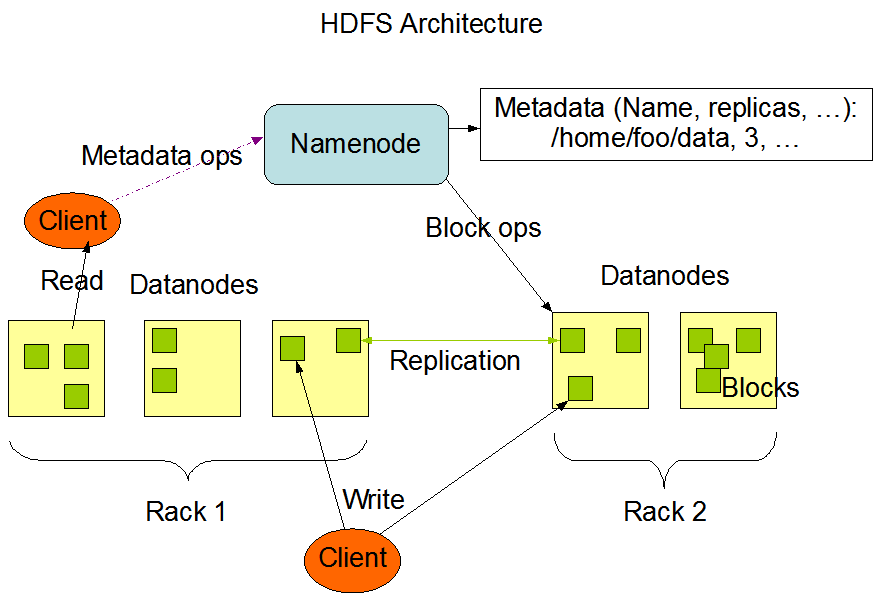
\includegraphics[width=1\textwidth]{hdfsarchitecture}}
\caption{Архитектура HDFS}
\label{fig:hdfsarchitecture}
\end{figure}

\begin{itemize}
\item \textbf{Namenode}

Этот компонент системы осуществляет всю работу с метаданными. Он должен быть запущен только на одном компьютере 
в кластере. Именно он управляет размещением информации и доступом ко всем данным, расположенным на ресурсах кластера. 
Сами данные проходят с остальных машин кластера к клиенту мимо него.

\item \textbf{Datanode}

На всех остальных компьютерах системы работает именно этот компонент. Он располагает сами блоки данных в локальной 
файловой системе для последующей передачи или обработки их по запросу клиента. Группы узлов данных принято называть 
Rack, они используются, например, в схемах репликации данных.

\item \textbf{Клиент}

Просто приложение или пользователь, работающий с файловой системой. В его роли может выступать практически что угодно.
\end{itemize}

Пространство имен HDFS имеет классическую иерархическую структуру: пользователи и приложения имеют возможность 
создавать директории и файлы. Файлы хранятся в виде блоков данных произвольной (но одинаковой, за исключением последнего; 
по-умолчанию 64 mb) длины, размещенных на Datanode'ах. Для обеспечения отказоустойчивости блоки хранятся в нескольких 
экземплярах на разных узлах, имеется возможность настройки количества копий и алгоритма их распределения по системе. 
Удаление файлов происходит не сразу, а через какое-то время после соответствующего запроса, так как после получения 
запроса файл перемещается в директорию /trash и хранится там определенный период времени на случай если пользователь 
или приложение передумают о своем решении. В этом случае информацию можно будет восстановить, в противном случае~--- физически удалить.

Для обнаружения возникновения каких-либо неисправностей, Datanode периодически отправляют Namenode'у сигналы о 
своей работоспособности. При прекращении получения таких сигналов от одного из узлов Namenode помечает его как <<мертвый>>, 
и прекращает какой-либо с ним взаимодействие до возвращения его работоспособности. Данные, хранившиеся на <<умершем>> узле 
реплицируются дополнительный раз из оставшихся <<в живых>> копий и система продолжает свое функционирование как ни в чем не бывало.

Все коммуникации между компонентами файловой системы проходят по специальным протоколам, основывающимся на стандартном TCP/IP. 
Клиенты работают с Namenode с помощью так называемого ClientProtocol, а передача данных происходит по DatanodeProtocol, 
оба они обернуты в Remote Procedure Call (RPC).

Система предоставляет несколько интерфейсов, среди которых командная оболочка DFSShell, набор ПО для администрирования DFSAdmin, 
а также простой, но эффективный веб-интерфейс. Помимо этого существуют несколько API для языков программирования: Java API, 
C pipeline, WebDAV и так далее.

\textbf{MapReduce}

Помимо файловой системы, Hadoop включает в себя framework для проведения масштабных вычислений, обрабатывающих 
огромные объемы данных. Каждое такое вычисление называется Job (задание) и состоит оно, как видно из названия, из двух этапов:

\begin{itemize}
\item \textbf{Map}

Целью этого этапа является представление произвольных данных (на практике чаще всего просто пары ключ-значение) в виде 
промежуточных пар ключ-значение. Результаты сортируются и групируются по ключу и передаются на следующий этап.

\item \textbf{Reduce}

Полученные после map значения используются для финального вычисления требуемых данных. Практические любые данные могут 
быть получены таким образом, все зависит от требований и функционала приложения.
\end{itemize}

Задания выполняются, подобно файловой системе, на всех машинах в кластере (чаще всего одних и тех же). Одна из них выполняет 
роль управления работой остальных — JobTracker, остальные же ее бесприкословно слушаются — TaskTracker. В задачи 
JobTracker'а входит составление расписания выполняемых работ, наблюдение за ходом выполнения, и перераспределение в случае 
возникновения сбоев.

В общем случае каждое приложение, работающее с этим framework'ом, предоставляет методы для осуществления этапов map и reduce, 
а также указывает расположения входных и выходных данных. После получения этих данных JobTracker распределяет задание между 
остальными машинами и предоставляет клиенту полную информацию о ходе работ.

Помимо основных вычислений могут выполняться вспомогательные процессы, такие как составление отчетов о ходе работы, кэширование, 
сортировка и так далее.

\textbf{HBase}

В рамках Hadoop доступна еще и система хранения данных, которую правда сложно назвать СУБД в традиционном смысле этого слова. 
Чаще проводят аналогии с проприетарной системой этого же плана от Google~--- BigTable.

HBase представляет собой распределенную систему хранения больших объемов данных. Подобно реляционным СУБД данные хранятся в 
виде таблиц, состоящих из строк и столбцов. И даже для доступа к ним предоставляется язык запросов HQL (как ни странно~--- 
Hadoop Query Language), отдаленно напоминающий более распространенный SQL. Помимо этого предоставляется итерирующмй интерфейс 
для сканирования наборов строк.

Одной из основных особенностей хранения данных в HBase является возможность наличия нескольких значений, 
соответствующих одной комбинации таблица-строка-столбец, для их различения используется информация о времени добавления записи. 
На концептуальном уровне таблицы обычно представляют как набор строк, но физически же они хранятся по столбцам, достаточно 
важный факт, который стоит учитывать при разработки схемы хранения данных. Пустые ячейки не отображаются каким-либо образом 
физически в хранимых данных, они просто отсутствуют. Существуют конечно и другие нюансы, но я постарался упомянуть лишь основные.

HQL очень прост по своей сути, если Вы уже знаете SQL, то для изучения его Вам понадобится лишь просмотреть по диагонали 
коротенький вывод команды help;, занимающий всего пару экранов в консоли. Все те же SELECT, INSERT, UPDATE, DROP и так далее, 
лишь со слегка измененным синтаксисом.

Помимо обычно командной оболочки HBase Shell, для работы с HBase также предоставлено несколько API для различных языков 
программирования: Java, Jython, REST и Thrift.

\textbf{HadoopDB}

В проекте HadoopDB специалисты из университетов Yale и Brown предпринимают попытку создать гибридную систему управления 
данными, сочетающую преимущества технологий и MapReduce, и параллельных СУБД. В их подходе MapReduce обеспечивает коммуникационную 
инфраструктуру, объединяющую произвольное число узлов, в которых выполняются экземпляры традиционной СУБД. Запросы формулируются 
на языке SQL, транслируются в среду MapReduce, и значительная часть работы передается в экземпляры СУБД. Наличие MapReduce 
обеспечивается масштабируемость и отказоустойчивость, а использование в узлах кластера СУБД позволяет добиться высокой 
производительности. 


\subsection{Установка и настройка}
Вся настройка ведется на Ubuntu Server операционной системе.

\subsubsection{Установка Hadoop}
Перед тем, как приступить собственно говоря к установке Hadoop, необходимо выполнить два элементарных действия, 
необходимых для правильного функционирования системы:
\begin{itemize}
\item открыть доступ одному из пользователей по ssh к этому же компьютеру без пароля, 
можно например создать отдельного пользователя для этого [hadoop]:
\begin{lstlisting}[label=lst:haddop1,caption=Создаем пользователя с правами]
$sudo groupadd hadoop
$sudo useradd -m -g hadoop -d /home/hadoop -s /bin/bash \
-c "Hadoop software owner" hadoop
\end{lstlisting}

Далее действия выполняем от его имени:
\begin{lstlisting}[label=lst:haddop2,caption=Логинимся под пользователем hadoop]
su hadoop
\end{lstlisting}

Генерим RSA-ключ для обеспечения аутентификации в условиях отсутствия возможности использовать пароль:
\begin{lstlisting}[label=lst:haddop3,caption=Генерим RSA-ключ]
hadoop@localhost ~ $ ssh-keygen -t rsa -P ""
Generating public/private rsa key pair.
Enter file in which to save the key (/home/hadoop/.ssh/id_rsa):
Your identification has been saved in /home/hadoop/.ssh/id_rsa.
Your public key has been saved in /home/hadoop/.ssh/id_rsa.pub.
The key fingerprint is:
7b:5c:cf:79:6b:93:d6:d6:8d:41:e3:a6:9d:04:f9:85 hadoop@localhost
\end{lstlisting}

И добавляем его в список авторизованных ключей:
\begin{lstlisting}[label=lst:haddop4,caption=Добавляем его в список авторизованных ключей]
cat $HOME/.ssh/id_rsa.pub >> $HOME/.ssh/authorized_keys
\end{lstlisting}

Этого должно быть более чем достаточно, проверить работоспособность соединения можно просто написав:
\begin{lstlisting}[label=lst:haddop5,caption=Пробуем зайти на ssh без пароля]
ssh localhost
\end{lstlisting}

Не забываем предварительно инициализировать sshd:
\begin{lstlisting}[label=lst:haddop6,caption=Запуск sshd]
/etc/init.d/sshd start
\end{lstlisting}

\item Помимо этого необходимо убедиться в наличии установленной JVM версии 1.5.0 или выше.
\begin{lstlisting}[label=lst:haddop7,caption=Устанавливаем JVM]
sudo aptitude install openjdk-6-jdk
\end{lstlisting}
\end{itemize}

Дальше скачиваем и устанавливаем Hadoop:
\begin{lstlisting}[label=lst:haddop8,caption=Устанавливаем Hadoop]
cd /opt
sudo wget http://www.gtlib.gatech.edu/pub/apache/hadoop
/core/hadoop-0.20.2/hadoop-0.20.2.tar.gz
sudo tar zxvf hadoop-0.20.2.tar.gz
sudo ln -s /opt/hadoop-0.20.2 /opt/hadoop
sudo chown -R hadoop:hadoop /opt/hadoop /opt/hadoop-0.20.2
sudo mkdir -p /opt/hadoop-data/tmp-base
sudo chown -R hadoop:hadoop /opt/hadoop-data/
\end{lstlisting}

Далее переходим в /opt/hadoop/conf/hadoop-env.sh и добавляем вначале:
\begin{lstlisting}[label=lst:haddop9,caption=Указываем переменные окружения]
export JAVA_HOME=/usr/lib/jvm/java-6-openjdk
export HADOOP_HOME=/opt/hadoop
export HADOOP_CONF=$HADOOP_HOME/conf
export HADOOP_PATH=$HADOOP_HOME/bin
export HIVE_HOME=/opt/hive
export HIVE_PATH=$HIVE_HOME/bin

export PATH=$HIVE_PATH:$HADOOP_PATH:$PATH
\end{lstlisting}

Далее добавим в /opt/hadoop/conf/hadoop-site.xml:
\begin{lstlisting}[language=XML,label=lst:haddop10,caption=Настройки hadoop]
<configuration>
<property>
  <name>hadoop.tmp.dir</name>
  <value>/opt/hadoop-data/tmp-base</value>
  <description>A base for other temporary directories</description>
</property>

<property>
  <name>fs.default.name</name>
  <value>localhost:54311</value>
  <description>
    The name of the default file system.
  </description>
</property>

<property>
  <name>hadoopdb.config.file</name>
  <value>HadoopDB.xml</value>
  <description>The name of the HadoopDB 
  cluster configuration file</description>
</property>
</configuration>
\end{lstlisting}

В /opt/hadoop/conf/mapred-site.xml:
\begin{lstlisting}[language=XML,label=lst:haddop11,caption=Настройки mapreduce]
<configuration>
<property>
  <name>mapred.job.tracker</name>
  <value>localhost:54310</value>
  <description>
    The host and port that the 
    MapReduce job tracker runs at.
  </description>
</property>
</configuration>
\end{lstlisting}

В /opt/hadoop/conf/hdfs-site.xml:
\begin{lstlisting}[language=XML,label=lst:haddop12,caption=Настройки hdfs]
<configuration>
<property>
  <name>dfs.replication</name>
  <value>1</value>
  <description>
    Default block replication.
  </description>
</property>
</configuration>
\end{lstlisting}

Теперь необходимо отформатировать Namenode:
\begin{lstlisting}[label=lst:haddop13,caption=Форматирование Namenode]
$ hadoop namenode -format
10/05/07 14:24:12 INFO namenode.NameNode: STARTUP_MSG: 
/************************************************************
STARTUP_MSG: Starting NameNode
STARTUP_MSG:   host = hadoop1/127.0.1.1
STARTUP_MSG:   args = [-format]
STARTUP_MSG:   version = 0.20.2
STARTUP_MSG:   build = https://svn.apache.org/repos
/asf/hadoop/common/branches/branch-0.20 -r
911707; compiled by 'chrisdo' on Fri Feb 19 08:07:34 UTC 2010
************************************************************/
10/05/07 14:24:12 INFO namenode.FSNamesystem: 
fsOwner=hadoop,hadoop
10/05/07 14:24:12 INFO namenode.FSNamesystem: 
supergroup=supergroup
10/05/07 14:24:12 INFO namenode.FSNamesystem: 
isPermissionEnabled=true
10/05/07 14:24:12 INFO common.Storage: 
Image file of size 96 saved in 0 seconds.
10/05/07 14:24:12 INFO common.Storage: 
Storage directory /opt/hadoop-data/tmp-base/dfs/name has been
successfully formatted.
10/05/07 14:24:12 INFO namenode.NameNode: 
SHUTDOWN_MSG: 
/************************************************************
SHUTDOWN_MSG: Shutting down NameNode at hadoop1/127.0.1.1
************************************************************/
\end{lstlisting}

Готово. Теперь мы можем запустить Hadoop:
\begin{lstlisting}[label=lst:haddop14,caption=Запуск Hadoop]
$ start-all.sh
starting namenode, logging to /opt/hadoop/bin/..
/logs/hadoop-hadoop-namenode-hadoop1.out
localhost: starting datanode, logging to 
/opt/hadoop/bin/../logs/hadoop-hadoop-datanode-hadoop1.out
localhost: starting secondarynamenode, logging to
/opt/hadoop/bin/../logs/hadoop-hadoop-secondarynamenode-hadoop1.out
starting jobtracker, logging to 
/opt/hadoop/bin/../logs/hadoop-hadoop-jobtracker-hadoop1.out
localhost: starting tasktracker, logging to
/opt/hadoop/bin/../logs/hadoop-hadoop-tasktracker-hadoop1.out
\end{lstlisting}

Остановка Hadoop производится скриптом stop-all.sh.

\subsubsection{Установка HadoopDB и Hive}
Теперь скачаем HaddopDB\footnote{http://sourceforge.net/projects/hadoopdb/files/} и распакуем hadoopdb.jar в \$HADOOP\_HOME/lib:
\begin{lstlisting}[label=lst:haddop15,caption=Установка HadoopDB]
$cp hadoopdb.jar $HADOOP_HOME/lib
\end{lstlisting}

Также нам потребуется PostgreSQL JDBC библиотека. Скачайте её\footnote{http://jdbc.postgresql.org/download.html} и 
распакуйте в директорию \$HADOOP\_HOME/lib.

Hive используется HadoopDB как SQL интерфейс. Подготовим директорию в HDFS для Hive:
\begin{lstlisting}[label=lst:haddop16,caption=Установка HadoopDB]
hadoop fs -mkdir /tmp
hadoop fs -mkdir /user/hive/warehouse
hadoop fs -chmod g+w /tmp
hadoop fs -chmod g+w /user/hive/warehouse
\end{lstlisting}

В архиве HadoopDB также есть архив SMS\_dist. Распакуем его:
\begin{lstlisting}[label=lst:haddop17,caption=Установка HadoopDB]
tar zxvf SMS_dist.tar.gz
sudo mv dist /opt/hive
sudo chown -R hadoop:hadoop hive
\end{lstlisting}

Поскольку мы успешно запустили Hadoop, то и проблем с запуском Hive не должно быть:
\begin{lstlisting}[label=lst:haddop18,caption=Установка HadoopDB]
$ hive
Hive history file=/tmp/hadoop/
hive_job_log_hadoop_201005081717_1990651345.txt
hive> 

hive> quit;
\end{lstlisting}

\subsubsection{Тестирование}
Теперь проведем тестирование. Для этого скачаем бенчмарк:
\begin{lstlisting}[label=lst:haddop19,caption=Тестирование]
svn co http://graffiti.cs.brown.edu/svn/benchmarks/
cd benchmarks/datagen/teragen
\end{lstlisting}

Изменим скрипт benchmarks/datagen/teragen/teragen.pl к виду:
\begin{lstlisting}[language=Java,label=lst:haddop20,caption=Тестирование]
use strict;
use warnings;

my $CUR_HOSTNAME = `hostname -s`;
chomp($CUR_HOSTNAME);

my $NUM_OF_RECORDS_1TB    = 10000000000;
my $NUM_OF_RECORDS_535MB  = 100;
my $BASE_OUTPUT_DIR   = "/data";
my $PATTERN_STRING    = "XYZ";
my $PATTERN_FREQUENCY = 108299;
my $TERAGEN_JAR       = "teragen.jar";
my $HADOOP_COMMAND    = $ENV{'HADOOP_HOME'}."/bin/hadoop";

my %files = ( "535MB" => 1,
);
system("$HADOOP_COMMAND fs -rmr $BASE_OUTPUT_DIR");
foreach my $target (keys %files) {
my $output_dir = $BASE_OUTPUT_DIR."/SortGrep$target";
my $num_of_maps = $files{$target};
my $num_of_records = ($target eq "535MB" ? 
$NUM_OF_RECORDS_535MB : $NUM_OF_RECORDS_1TB);
print "Generating $num_of_maps files in '$output_dir'\n";

##
## EXEC: hadoop jar teragen.jar 10000000000 
## /data/SortGrep/ XYZ 108299 100
##
my @args = ( $num_of_records,
	    $output_dir,
	    $PATTERN_STRING,
	    $PATTERN_FREQUENCY,
	    $num_of_maps );
my $cmd = "$HADOOP_COMMAND jar $TERAGEN_JAR ".join(" ", @args);
print "$cmd\n";
system($cmd) == 0 || die("ERROR: $!");
} # FOR
exit(0);
\end{lstlisting}

При запуске данного Perl скрипта сгенерится данные, которые будут сохранены на HDFS. 
Поскольку мы настроили систему как единственный кластер, то все данные будут загружены на один HDFS. 
При работе с большим количеством кластеров данные были бы распределены по кластерам.
Создадим базу данных, таблицу и загрузим данные, что мы сохранили на HDFS, в нее:
\begin{lstlisting}[label=lst:haddop21,caption=Тестирование]
$hadoop fs -get /data/SortGrep535MB/part-00000 my_file
$psql
psql> CREATE DATABASE grep0;
psql> USE grep0;
psql> CREATE TABLE grep (
    ->   key1 character varying(255),
    ->   field character varying(255)
    -> );
COPY grep FROM 'my_file' WITH DELIMITER '|';
\end{lstlisting}

Теперь настроим HadoopDB. В архиве HadoopDB можно найти пример файла Catalog.properties. Распакуйт его и настройте:
\begin{lstlisting}[label=lst:haddop22,caption=Тестирование]
#Properties for Catalog Generation
##################################
nodes_file=machines.txt
relations_unchunked=grep, EntireRankings
relations_chunked=Rankings, UserVisits
catalog_file=HadoopDB.xml
##
#DB Connection Parameters
##
port=5432
username=postgres
password=password
driver=com.postgresql.Driver
url_prefix=jdbc\:postgresql\://
##
#Chunking properties
##
chunks_per_node=0
unchunked_db_prefix=grep
chunked_db_prefix=cdb
##
#Replication Properties
##
dump_script_prefix=/root/dump_
replication_script_prefix=/root/load_replica_
dump_file_u_prefix=/mnt/dump_udb
dump_file_c_prefix=/mnt/dump_cdb
##
#Cluster Connection
##
ssh_key=id_rsa
\end{lstlisting}

Создайте файл machines.txt и добавте туда <<localhost>> строчку (без кавычек). Тепер создадим HadoopDB конфиг и скопируем его в HDFS:
\begin{lstlisting}[label=lst:haddop23,caption=Тестирование]
java -cp $HADOOP_HOME/lib/hadoopdb.jar \
> edu.yale.cs.hadoopdb.catalog.SimpleCatalogGenerator \
> Catalog.properties
hadoop dfs -put HadoopDB.xml HadoopDB.xml
\end{lstlisting}

Также возможно создать конфиг для создания репликации командой:
\begin{lstlisting}[label=lst:haddop23:1,caption=Репликация]
java -cp hadoopdb.jar edu.yale.cs.hadoopdb.catalog.SimpleRandomReplicationFactorTwo Catalog.properties
\end{lstlisting}

Инструмент генерирует новый файл HadoopDB.xml, в котором случайные порции данных реплицируются на все узлы.
После этого не забываем обновить конфиг на HDFS:
\begin{lstlisting}[label=lst:haddop23:2,caption=Обновляем конфиг]
hadoop dfs -rmr HadoopDB.xml
hadoop dfs -put HadoopDB.xml HadoopDB.xml
\end{lstlisting}
и поставить <<true>> для <<hadoopdb.config.replication>> в HADOOP\_HOME/conf/hadoop-site.xml.

Теперь мы готовы проверить работы HadoopDB. Теперь можем протестировать поиск по данным, загруженым ранее в БД и HDFS:
\begin{lstlisting}[label=lst:haddop24,caption=Тестирование]
java -cp $CLASSPATH:hadoopdb.jar \
> edu.yale.cs.hadoopdb.benchmark.GrepTaskDB \
> -pattern %wo% -output padraig -hadoop.config.file HadoopDB.xml
\end{lstlisting}

Приблизительный результат:
\begin{lstlisting}[label=lst:haddop25,caption=Тестирование]
$java -cp $CLASSPATH:hadoopdb.jar edu.yale.cs.hadoopdb.benchmark.GrepTaskDB \
> -pattern %wo% -output padraig -hadoop.config.file HadoopDB.xml
14.08.2010 19:08:48 edu.yale.cs.hadoopdb.exec.DBJobBase initConf
INFO: SELECT key1, field FROM grep WHERE field LIKE '%%wo%%';
14.08.2010 19:08:48 org.apache.hadoop.metrics.jvm.JvmMetrics init
INFO: Initializing JVM Metrics with processName=JobTracker, sessionId=
14.08.2010 19:08:48 org.apache.hadoop.mapred.JobClient configureCommandLineOptions
WARNING: Use GenericOptionsParser for parsing the arguments. 
Applications should implement Tool for the same.
14.08.2010 19:08:48 org.apache.hadoop.mapred.JobClient monitorAndPrintJob
INFO: Running job: job_local_0001
14.08.2010 19:08:48 edu.yale.cs.hadoopdb.connector.AbstractDBRecordReader getConnection
INFO: Data locality failed for leo-pgsql
14.08.2010 19:08:48 edu.yale.cs.hadoopdb.connector.AbstractDBRecordReader getConnection
INFO: Task from leo-pgsql is connecting to chunk 0 on host localhost with 
db url jdbc:postgresql://localhost:5434/grep0
14.08.2010 19:08:48 org.apache.hadoop.mapred.MapTask runOldMapper
INFO: numReduceTasks: 0
14.08.2010 19:08:48 edu.yale.cs.hadoopdb.connector.AbstractDBRecordReader close
INFO: DB times (ms): connection = 104, query execution = 20, row retrieval  = 79
14.08.2010 19:08:48 edu.yale.cs.hadoopdb.connector.AbstractDBRecordReader close
INFO: Rows retrieved = 3
14.08.2010 19:08:48 org.apache.hadoop.mapred.Task done
INFO: Task:attempt_local_0001_m_000000_0 is done. And is in the process of commiting
14.08.2010 19:08:48 org.apache.hadoop.mapred.LocalJobRunner$Job statusUpdate
INFO: 
14.08.2010 19:08:48 org.apache.hadoop.mapred.Task commit
INFO: Task attempt_local_0001_m_000000_0 is allowed to commit now
14.08.2010 19:08:48 org.apache.hadoop.mapred.FileOutputCommitter commitTask
INFO: Saved output of task 'attempt_local_0001_m_000000_0' to file:/home/leo/padraig
14.08.2010 19:08:48 org.apache.hadoop.mapred.LocalJobRunner$Job statusUpdate
INFO: 
14.08.2010 19:08:48 org.apache.hadoop.mapred.Task sendDone
INFO: Task 'attempt_local_0001_m_000000_0' done.
14.08.2010 19:08:49 org.apache.hadoop.mapred.JobClient monitorAndPrintJob
INFO:  map 100% reduce 0%
14.08.2010 19:08:49 org.apache.hadoop.mapred.JobClient monitorAndPrintJob
INFO: Job complete: job_local_0001
14.08.2010 19:08:49 org.apache.hadoop.mapred.Counters log
INFO: Counters: 6
14.08.2010 19:08:49 org.apache.hadoop.mapred.Counters log
INFO:   FileSystemCounters
14.08.2010 19:08:49 org.apache.hadoop.mapred.Counters log
INFO:     FILE_BYTES_READ=141370
14.08.2010 19:08:49 org.apache.hadoop.mapred.Counters log
INFO:     FILE_BYTES_WRITTEN=153336
14.08.2010 19:08:49 org.apache.hadoop.mapred.Counters log
INFO:   Map-Reduce Framework
14.08.2010 19:08:49 org.apache.hadoop.mapred.Counters log
INFO:     Map input records=3
14.08.2010 19:08:49 org.apache.hadoop.mapred.Counters log
INFO:     Spilled Records=0
14.08.2010 19:08:49 org.apache.hadoop.mapred.Counters log
INFO:     Map input bytes=3
14.08.2010 19:08:49 org.apache.hadoop.mapred.Counters log
INFO:     Map output records=3
14.08.2010 19:08:49 edu.yale.cs.hadoopdb.exec.DBJobBase run
INFO: 
JOB TIME : 1828 ms.

\end{lstlisting}

Результат сохранен в HDFS, в папке padraig:
\begin{lstlisting}[label=lst:haddop26,caption=Тестирование]
$ cd padraig
$ cat part-00000
some data
\end{lstlisting}

Проверим данные в PostgreSQL:
\begin{lstlisting}[label=lst:haddop27,caption=Тестирование]
psql> select * from grep where field like '%wo%';
+--------------------------------+-------------------+
| key1                           | field
|
+--------------------------------+-------------------+
some data

1 rows in set (0.00 sec)

psql>
\end{lstlisting}

Значения совадают. Все работает как требуется.

Проведем еще один тест. Добавим данные в PostgreSQL:
\begin{lstlisting}[label=lst:haddop27:1,caption=Тестирование]
psql> INSERT into grep(key1, field) VALUES('I am live!', 'Maybe');
psql> INSERT into grep(key1, field) VALUES('I am live!', 'Maybewqe');
psql> INSERT into grep(key1, field) VALUES('I am live!', 'Maybewqesad');
psql> INSERT into grep(key1, field) VALUES(':)', 'May cool string!');
\end{lstlisting}

Теперь проверим через HadoopDB:
\begin{lstlisting}[label=lst:haddop27:2,caption=Тестирование]
$ java -cp $CLASSPATH:hadoopdb.jar edu.yale.cs.hadoopdb.benchmark.GrepTaskDB -pattern %May% -output padraig -hadoopdb.config.file /opt/hadoop/conf/HadoopDB.xml
padraig
01.11.2010 23:14:45 edu.yale.cs.hadoopdb.exec.DBJobBase initConf
INFO: SELECT key1, field FROM grep WHERE field LIKE '%%May%%';
01.11.2010 23:14:46 org.apache.hadoop.metrics.jvm.JvmMetrics init
INFO: Initializing JVM Metrics with processName=JobTracker, sessionId=
01.11.2010 23:14:46 org.apache.hadoop.mapred.JobClient configureCommandLineOptions
WARNING: Use GenericOptionsParser for parsing the arguments. Applications should implement Tool for the same.
01.11.2010 23:14:46 org.apache.hadoop.mapred.JobClient monitorAndPrintJob
INFO: Running job: job_local_0001
01.11.2010 23:14:46 edu.yale.cs.hadoopdb.connector.AbstractDBRecordReader getConnection
INFO: Data locality failed for leo-pgsql
01.11.2010 23:14:46 edu.yale.cs.hadoopdb.connector.AbstractDBRecordReader getConnection
INFO: Task from leo-pgsql is connecting to chunk 0 on host localhost with db url jdbc:postgresql://localhost:5434/grep0
01.11.2010 23:14:47 org.apache.hadoop.mapred.MapTask runOldMapper
INFO: numReduceTasks: 0
01.11.2010 23:14:47 edu.yale.cs.hadoopdb.connector.AbstractDBRecordReader close
INFO: DB times (ms): connection = 181, query execution = 22, row retrieval  = 96
01.11.2010 23:14:47 edu.yale.cs.hadoopdb.connector.AbstractDBRecordReader close
INFO: Rows retrieved = 4
01.11.2010 23:14:47 org.apache.hadoop.mapred.Task done
INFO: Task:attempt_local_0001_m_000000_0 is done. And is in the process of commiting
01.11.2010 23:14:47 org.apache.hadoop.mapred.LocalJobRunner$Job statusUpdate
INFO: 
01.11.2010 23:14:47 org.apache.hadoop.mapred.Task commit
INFO: Task attempt_local_0001_m_000000_0 is allowed to commit now
01.11.2010 23:14:47 org.apache.hadoop.mapred.FileOutputCommitter commitTask
INFO: Saved output of task 'attempt_local_0001_m_000000_0' to file:/home/hadoop/padraig
01.11.2010 23:14:47 org.apache.hadoop.mapred.LocalJobRunner$Job statusUpdate
INFO: 
01.11.2010 23:14:47 org.apache.hadoop.mapred.Task sendDone
INFO: Task 'attempt_local_0001_m_000000_0' done.
01.11.2010 23:14:47 org.apache.hadoop.mapred.JobClient monitorAndPrintJob
INFO:  map 100% reduce 0%
01.11.2010 23:14:47 org.apache.hadoop.mapred.JobClient monitorAndPrintJob
INFO: Job complete: job_local_0001
01.11.2010 23:14:47 org.apache.hadoop.mapred.Counters log
INFO: Counters: 6
01.11.2010 23:14:47 org.apache.hadoop.mapred.Counters log
INFO:   FileSystemCounters
01.11.2010 23:14:47 org.apache.hadoop.mapred.Counters log
INFO:     FILE_BYTES_READ=141345
01.11.2010 23:14:47 org.apache.hadoop.mapred.Counters log
INFO:     FILE_BYTES_WRITTEN=153291
01.11.2010 23:14:47 org.apache.hadoop.mapred.Counters log
INFO:   Map-Reduce Framework
01.11.2010 23:14:47 org.apache.hadoop.mapred.Counters log
INFO:     Map input records=4
01.11.2010 23:14:47 org.apache.hadoop.mapred.Counters log
INFO:     Spilled Records=0
01.11.2010 23:14:47 org.apache.hadoop.mapred.Counters log
INFO:     Map input bytes=4
01.11.2010 23:14:47 org.apache.hadoop.mapred.Counters log
INFO:     Map output records=4
01.11.2010 23:14:47 edu.yale.cs.hadoopdb.exec.DBJobBase run
INFO: 
JOB TIME : 2332 ms.
\end{lstlisting}

Как паттерн поиска я задал <<May>>. В логах можно увидеть как производится поиск. На выходе получаем:
\begin{lstlisting}[label=lst:haddop27:3,caption=Тестирование]
$ cd padraig
$ cat part-00000
I am live!	Maybe
I am live!	Maybewqe
I am live!	Maybewqesad
:)	May cool string!
\end{lstlisting}

В упрощенной системе с одним кластером PostgreSQL не понятно ради чего такие сложности. 
Но если к HadoopDB подключить более одного кластера PostgreSQL, 
то данной методикой возможно работать с данными PostgreSQL, объединенных в shared-nothing кластер.

Более подробно по HadoopDB можно почитать по данной ссылке \\http://hadoopdb.sourceforge.net/guide/quick\_start\_guide.html.


\subsection{Заключение}
В данной статье не показывается, как работать с Hive, как более проще работать с HadoopDB. Эта книга не сможет учесть все, 
что требуется для работы c Hadoop. Назначение этой главы~--- дать основу для работы с Hadoop и HaddopDB.

HadoopDB не заменяет Hadoop. Эти системы сосуществуют, позволяя аналитику выбирать соответствующие средства в зависимости 
от имеющихся данных и задач.

HadoopDB может приблизиться в отношении производительности к параллельным системам 
баз данных, обеспечивая при этом отказоустойчивость и возможность использования в неоднородной среде при тех же правилах 
лицензирования, что и Hadoop. Хотя производительность HadoopDB, вообще говоря, ниже производительности параллельных систем 
баз данных, во многом это объясняется тем, что в PostgreSQL таблицы хранятся не по столбцам, и тем, что в PostgreSQL 
не использовалось сжатие данных. Кроме того, Hadoop и Hive~--- это сравнительно молодые проекты с открытыми кодами. 

В HadoopDB применяется некоторый гибрид подходов параллельных СУБД и Hadoop к анализу данных, позволяющий достичь производительности 
и эффективности параллельных систем баз данных, обеспечивая при этом масштабируемсть, отказоустойчивость и гибкость систем, 
основанных на MapReduce. Способность HadoopDB к прямому включению Hadoop и программного обеспечения СУБД с открытыми исходными 
текстами (без изменения кода) делает HadoopDB особенно пригодной для выполнения крупномасштабного анализа данных в будущих 
рабочих нагрузках.
\section{Заключение}
В данной главе расмотрено лиш базовые настройки кластеров БД. 
Про кластеры PostgreSQL потребуется написать отдельную книгу, чтобы растмотреть все шаги с установкой, настройкой и работой кластеров.
Надеюсь, что несмотря на это, информация будет полезна многим читателям.
%clustering end
%pgpool begin
\chapter{PgPool-II}
\begin{epigraphs}
\qitem{Имеется способ сделать лучше~--- найди его.}{Томас Алва Эдисон}
\end{epigraphs}
\section{Введение}
pgpool-II это прослойка, работающая между серверами PostgreSQL и клиентами СУБД PostgreSQL. 
Она предоставляет следующие функции:
\begin{itemize}
\item \textbf{Объединение соединений} 

pgpool-II сохраняет соединения с серверами PostgreSQL и использует их повторно в случае если новое 
соединение устанавливается с теми же параметрами (т.е. имя пользователя, база данных, версия протокола). 
Это уменьшает накладные расходы на соединения и увеличивает производительность системы вцелом.

\item \textbf{Репликация} 

pgpool-II может управлять множеством серверов PostgreSQL. Использование функции репликации данных позволяет 
создание резервной копии данных в реальном времени на  2 или более физических дисков, так что сервис может 
продолжать работать без остановки серверов в случае выхода из строя диска.

\item \textbf{Балансировка нагрузки}

Если база данных реплицируется, то выполнение запроса SELECT на любом из серверов вернет одинаковый результат. 
pgpool-II использует преимущество функции репликации для уменьшения нагрузки на каждый из серверов PostgreSQL 
распределяя запросы SELECT на несколько серверов, тем самым увеличивая производительность системы вцелом. 
В лучшем случае производительность возрастает пропорционально числу серверов PostgreSQL. Балансировка нагрузки 
лучше всего работает в случае когда много пользователей выполняют много запросов в одно и тоже время.

\item \textbf{Ограничение лишних соединений}

Существует ограничение максимального числа одновременных соединений с PostgreSQL, при превышении которого новые 
соединения отклоняются. Установка максимального числа соединений, в то же время, увеличивает потребление ресурсов и 
снижает производительность системы. pgpool-II также имеет ограничение на максимальное число соединений, но <<лишние>> 
соединения будут поставлены в очередь вместо немедленного возврата ошибки.

\item \textbf{Параллельные запросы}

Используя функцию параллельных запросов можно разнести данные на множество серверов, благодаря чему запрос может 
быть выполнен на всех серверах одновременно для уменьшения общего времени выполнения. Параллельные запросы работают 
лучше всего при поиске в больших объемах данных.
\end{itemize}

pgpool-II общается по протоколу бэкенда и фронтенда PostgreSQL и располагается между ними. 
Таким образом, приложение базы данных (фронтенд) считает что pgpool-II~--- настоящий сервер PostgreSQL, а сервер (бэкенд) 
видит pgpool-II как одного из своих клиентов. Поскольку pgpool-II прозрачен как для сервера, так и для клиента, 
существующие приложения, работающие с базой данных, могут использоваться с pgpool-II практически без изменений в исходном коде.

Оригинал руководства доступен по адресу http://pgpool.projects.postgresql.org/pgpool-II/doc/tutorial-en.html.

\section{Давайте начнем!}
\label{sec:pgpool-II-begin}
Перед тем как использовать репликацию или параллельные запросы мы должны научиться устанавливать и настраивать pgpool-II 
и узлы базы данных.

\subsection{Установка pgpool-II}
Установка pgpool-II очень проста. В каталоге, в который вы распаковали архив 
с исходными текстами, выполните следующие команды.
\begin{lstlisting}[label=lst:pgpool1,caption=Установка pgpool-II]
./configure
make
make install
\end{lstlisting}

Скрипт configure собирает информацию о вашей системе и использует ее в процедуре компиляции. Вы можете 
указать параметры в командной строке скрипта configure чтобы изменить его поведение по-умолчанию, такие, например, 
как каталог установки. pgpool-II по-умолчанию будет установлен в каталог /usr/local.

Команда make скомпилирует исходный код, а make install установит исполняемые файлы. У вас должно быть право на 
запись в каталог установки.

Обратите внимание: для работы pgpool-II необходима библиотека libpq для PostgreSQL 7.4 или более поздней версии (3 версия протокола).
Если скрипт configure выдает следующее сообщение об ошибке, возможно не установлена библиотека libpq или она не 3 версии.
\begin{lstlisting}[label=lst:pgpool2,caption=Установка pgpool-II]
configure: error: libpq is not installed or libpq is old
\end{lstlisting}

Если библиотека 3 версии, но указанное выше сообщение все-таки выдается, ваша библиотека libpq, вероятно, 
не распознается скриптом configure.

Скрипт configure ищет библиотеку libpq начиная от каталога /usr/local/pgsql. Если вы установили PostgreSQL в каталог 
отличный от /usr/local/pgsql используйте параметры командной строки --with-pgsql или --with-pgsql-includedir вместе с 
параметром --with-pgsql-libdir при запуске скрипта configure.

Во многих Linux системах pgpool-II может находится в репозитории пакетов. 
Для Ubuntu Linux, например, достаточно будет выполнить:
\begin{lstlisting}[label=lst:pgpool3,caption=Установка pgpool-II]
sudo aptitude install pgpool2
\end{lstlisting}

\subsection{Файлы конфигурации}
Параметры конфигурации pgpool-II хранятся в файле pgpool.conf. Формат файла: одна пара <<параметр = значение>> в строке. 
При установке pgpool-II автоматически создается файл pgpool.conf.sample. Мы рекомендуем скопировать его в файл pgpool.conf, 
а затем отредактировать по вашему желанию.
\begin{lstlisting}[label=lst:pgpool4,caption=Файлы конфигурации]
cp /usr/local/etc/pgpool.conf.sample /usr/local/etc/pgpool.conf
\end{lstlisting}

pgpool-II принимает соединения только с localhost на порт 9999. Если вы хотите принимать соединения с других хостов, 
установите для параметра listen\_addresses значение <<*>>.
\begin{lstlisting}[label=lst:pgpool5,caption=Файлы конфигурации]
listen_addresses = 'localhost'
port = 9999
\end{lstlisting}

Мы будем использовать параметры по-умолчанию в этом руководстве.

В Ubuntu Linux конфиг находится /etc/pgpool.conf.

\subsection{Настройка команд PCP}
У pgpool-II есть интерфейс для административных целей~--- получить информацию об узлах базы данных, 
остановить pgpool-II и т.д.~--- по сети. Чтобы использовать команды PCP, необходима идентификация пользователя. 
Эта идентификация отличается от идентификации пользователей в PostgreSQL. Имя пользователя и пароль нужно указывать в 
файле pcp.conf. В этом файле имя пользователя и пароль указываются как пара значений, разделенных двоеточием (:). 
Одна пара в строке. Пароли зашифрованы в формате хэша md5.
\begin{lstlisting}[label=lst:pgpool6,caption=Настройка команд PCP]
postgres:e8a48653851e28c69d0506508fb27fc5
\end{lstlisting}

При установке pgpool-II автоматически создается файл pcp.conf.sample. 
Мы рекомендуем скопировать его в файл pcp.conf и отредактировать.
\begin{lstlisting}[label=lst:pgpool7,caption=Настройка команд PCP]
$ cp /usr/local/etc/pcp.conf.sample /usr/local/etc/pcp.conf
\end{lstlisting}

В Ubuntu Linux файл находится /etc/pcp.conf.

Для того чтобы зашифровать ваш пароль в формате хэша md5 используете команду pg\_md5, которая устанавливается как один из 
исполняемых файлов pgpool-II. pg\_md5 принимает текст в параметре командной строки и отображает текст его md5 хэша.

Например, укажите <<postgres>> в качестве параметра командной строки и pg\_md5 выведет текст хэша md5 в стандартный поток вывода.
\begin{lstlisting}[label=lst:pgpool8,caption=Настройка команд PCP]
$ /usr/bin/pg_md5 postgres
e8a48653851e28c69d0506508fb27fc5
\end{lstlisting}

Команды PCP выполняются по сети, так что в файле pgpool.conf должен быть указан номер порта в параметре pcp\_port.

Мы будем использовать значение по-умолчанию для параметра pcp\_port 9898 в этом руководстве.
\begin{lstlisting}[label=lst:pgpool9,caption=Настройка команд PCP]
pcp_port = 9898
\end{lstlisting}


\subsection{Подготовка узлов баз данных}
Теперь нам нужно настроить серверы бэкендов PostgreSQL для pgpool-II. Эти серверы могут быть размещены на одном 
хосте с pgpool-II или на отдельных машинах. Если вы решите разместить серверы на том же хосте, для всех серверов 
должны быть установлены разные номера портов. Если серверы размещены на отдельных машинах, они должны быть настроены 
так чтобы могли принимать сетевые соединения от pgpool-II.

В этом руководстве мы разместили три сервера в рамках одного хоста вместе с pgpool-II и присвоили им номера портов 
5432, 5433, 5434 соответственно. Для настройки pgpool-II отредактируйте файл pgpool.conf как показано ниже.
\begin{lstlisting}[label=lst:pgpool10,caption=Подготовка узлов баз данных]
backend_hostname0 = 'localhost'
backend_port0 = 5432
backend_weight0 = 1
backend_hostname1 = 'localhost'
backend_port1 = 5433
backend_weight1 = 1
backend_hostname2 = 'localhost'
backend_port2 = 5434
backend_weight2 = 1
\end{lstlisting}

В параметрах backend\_hostname, backend\_port, backend\_weight укажите имя хоста узла базы данных, номер порта и 
коэффициент для балансировки нагрузки. В конце имени каждого параметра должен быть указан идентификатор узла путем 
добавления положительного целого числа начиная с 0 (т.е. 0, 1, 2).

Параметры backend\_weight все равны 1, что означает что запросы SELECT равномерно распределены по трем серверам.

\subsection{Запуск/Остановка pgpool-II}
Для старта pgpool-II выполните в терминале следующую команду.
\begin{lstlisting}[label=lst:pgpool11,caption=Запуск]
pgpool
\end{lstlisting}

Указанная выше команда, однако, не печатает протокол своей работы потому что pgpool отсоединяется от терминала. 
Если вы хотите показать протокол работы pgpool, укажите параметр -n в командной строке при запуске pgpool. 
pgpool-II будет запущен как процесс не-демон и терминал не будет отсоединен.
\begin{lstlisting}[label=lst:pgpool12,caption=Запуск]
pgpool -n &
\end{lstlisting}

Протокол работы будет печататься на терминал, так что рекомендуемые для использования параметры командной строки, 
например, такие.
\begin{lstlisting}[label=lst:pgpool13,caption=Запуск]
pgpool -n -d > /tmp/pgpool.log 2>&1 &
\end{lstlisting}

Параметр -d включает генерацию отладочных сообщений.

Указанная выше команда постоянно добавляет выводимый протокол работы в файл /tmp/pgpool.log. Если вам нужно 
ротировать файлы протоколов, передавайте протоколы внешней команде, у которой есть функция ротации протоколов. 
Вам поможет, например, cronolog.
\begin{lstlisting}[label=lst:pgpool14,caption=Запуск]
pgpool -n 2>&1 | /usr/sbin/cronolog
  --hardlink=/var/log/pgsql/pgpool.log
  '/var/log/pgsql/%Y-%m-%d-pgpool.log' &
\end{lstlisting}

Чтобы остановить процесс pgpool-II, выполните следующую команду.
\begin{lstlisting}[label=lst:pgpool15,caption=Остановка]
pgpool stop
\end{lstlisting}

Если какие-то из клиентов все еще присоединены, pgpool-II ждет пока они не отсоединятся и потом завершает свою работу. 
Если вы хотите завершить pgpool-II насильно, используйте вместо этой следующую команду.
\begin{lstlisting}[label=lst:pgpool16,caption=Остановка]
pgpool -m fast stop
\end{lstlisting}

\section{Ваша первая репликация}
\label{sec:pgpool-II-replica}
Репликация включает копирование одних и тех же данных на множество узлов базы данных.

В этом разделе мы будем использовать три узла базы данных, которые мы уже установили в разделе 
<<\ref{sec:pgpool-II-begin}. Давайте начнем!>>, и проведем вас шаг за шагом к созданию системы репликации базы данных. 
Пример данных для репликации будет сгенерирован программой для тестирования pgbench.

\subsection{Настройка репликации}
Чтобы включить функцию репликации базы данных установите значение true для параметра replication\_mode в файле pgpool.conf.
\begin{lstlisting}[label=lst:pgpool17,caption=Настройка репликации]
replication_mode = true
\end{lstlisting}

Если параметр replication\_mode равен true, pgpool-II будет отправлять копию принятого запроса на все узлы базы данных.

Если параметр load\_balance\_mode равен true, pgpool-II будет распределять запросы SELECT между узлами базы данных.
\begin{lstlisting}[label=lst:pgpool18,caption=Настройка репликации]
load_balance_mode = true
\end{lstlisting}

В этом разделе мы включили оба параметра replication\_mode и load\_balance\_mode.

\subsection{Проверка репликации}
Для отражения изменений, сделанных в файле pgpool.conf, pgpool-II должен быть перезапущен. 
Пожалуйста обращайтесь к разделу <<Запуск/Остановка pgpool-II>>.

После настройки pgpool.conf и перезапуска pgpool-II, давайте проверим репликацию в действии 
и посмотрим все ли работает хорошо.

Сначала нам нужно создать базу данных, которую будем реплицировать. Назовем ее <<bench\_replication>>. 
Эту базу данных нужно создать на всех узлах. Используйте команду createdb через pgpool-II и база 
данных будет создана на всех узлах.
\begin{lstlisting}[label=lst:pgpool19,caption=Проверка репликации]
createdb -p 9999 bench_replication
\end{lstlisting}

Затем мы запустим pgbench с параметром -i. Параметр -i инициализирует базу данных предопределенными 
таблицами и данными в них.
\begin{lstlisting}[label=lst:pgpool20,caption=Проверка репликации]
pgbench -i -p 9999 bench_replication
\end{lstlisting}

Указанная ниже таблица содержит сводную информацию о таблицах и данных, которые будут созданы при помощи pgbench -i. 
Если на всех узлах базы данных перечисленные таблицы и данные были созданы, репликация работает корректно.

\begin{tabular}{ | c | c | }
  \hline
  Имя таблицы & Число строк \\
  \hline
  branches & 1 \\
  \hline
  tellers & 10 \\
  \hline
  accounts & 100000 \\
  \hline
  history & 0 \\
  \hline
\end{tabular}

Для проверки указанной выше информации на всех узлах используем простой скрипт на shell. 
Приведенный ниже скрипт покажет число строк в таблицах branches, tellers, accounts и history 
на всех узлах базы данных (5432, 5433, 5434).
\begin{lstlisting}[label=lst:pgpool21,caption=Проверка репликации]
for port in 5432 5433 5434; do
>     echo $port
>     for table_name in branches tellers accounts history; do
>         echo $table_name
>         psql -c "SELECT count(*) FROM $table_name" -p \
>         $port bench_replication
>     done
> done
\end{lstlisting}


\section{Ваш первый параллельный запрос}
Данные из разных диапазонов сохраняются на двух или более узлах базы данных параллельным запросом. 
Это называется распределением (часто используется без перевода термин partitioning прим. переводчика). 
Более того, одни и те же данные на двух и более узлах базы данных могут быть воспроизведены с использованием распределения.

Чтобы включить параллельные запросы в pgpool-II вы должны установить еще одну базу данных, называемую 
<<Системной базой данных>> (<<System Database>>) (далее будем называть ее SystemDB).

SystemDB хранит определяемые пользователем правила, определяющие какие данные будут сохраняться на каких узлах бызы данных. 
Также SystemDB используется чтобы объединить результаты возвращенные узлами базы данных посредством dblink.

В этом разделе мы будем использовать три узла базы данных, которые мы установили в разделе <<\ref{sec:pgpool-II-begin}. 
Давайте начнем!>>, и проведем вас шаг за шагом к созданию системы баз данных с параллельными запросами. 
Для создания примера данных мы снова будем использовать pgbench.

\subsection{Настройка параллельного запроса}
Чтобы включить функцию выполнения параллельных запросов установите для параметра parallel\_mode значение true в файле pgpool.conf.
\begin{lstlisting}[label=lst:pgpool22,caption=Настройка параллельного запроса]
parallel_mode = true
\end{lstlisting}

Установка параметра parallel\_mode равным true не запустит параллельные запросы автоматически. 
Для этого pgpool-II нужна SystemDB и правила определяющие как распределять данные по узлам базы данных.

Также SystemDB использует dblink для создания соединений с pgpool-II. Таким образом, нужно установить значение 
параметра listen\_addresses таким образом чтобы pgpool-II принимал эти соединения.
\begin{lstlisting}[label=lst:pgpool23,caption=Настройка параллельного запроса]
listen_addresses = '*'
\end{lstlisting}

Внимание: Репликация не реализована для таблиц, которые распределяются посредством параллельных запросов и, 
в то же время, репликация может быть успешно осуществлена. Вместе с тем, из-за того что набор хранимых данных 
отличается при параллельных запросах и при репликации, база данных <<bench\_replication>>, созданная в разделе
<<\ref{sec:pgpool-II-replica}. Ваша первая репликация>> не может быть повторно использована.
\begin{lstlisting}[label=lst:pgpool24,caption=Настройка параллельного запроса]
replication_mode = true
load_balance_mode = false
\end{lstlisting}
ИЛИ
\begin{lstlisting}[label=lst:pgpool25,caption=Настройка параллельного запроса]
replication_mode = false
load_balance_mode = true
\end{lstlisting}

В этом разделе мы установим параметры parallel\_mode и load\_balance\_mode равными true, 
listen\_addresses равным <<*>>, replication\_mode равным false.


\subsection{Настройка SystemDB}
В основном, нет отличий между простой и системной базами данных. Однако, в системной базе данных определяется функция 
dblink и присутствует таблица, в которой хранятся правила распределения данных. Таблицу dist\_def необходимо определять. 
Более того, один из узлов базы данных может хранить системную базу данных, а pgpool-II может использоваться для 
распределения нагрузки каскадным подключеним.

В этом разделе мы создадим SystemDB на узле с портом 5432. Далее приведен список параметров конфигурации для SystemDB
\begin{lstlisting}[label=lst:pgpool26,caption=Настройка SystemDB]
system_db_hostname = 'localhost'
system_db_port = 5432
system_db_dbname = 'pgpool'
system_db_schema = 'pgpool_catalog'
system_db_user = 'pgpool'
system_db_password = ''
\end{lstlisting}

На самом деле, указанные выше параметры являются параметрами по-умолчанию в файле pgpool.conf. Теперь мы должны 
создать пользователя с именем <<pgpool>> и базу данных с именем <<pgpool>> и владельцем <<pgpool>>.
\begin{lstlisting}[label=lst:pgpool27,caption=Настройка SystemDB]
createuser -p 5432 pgpool
createdb -p 5432 -O pgpool pgpool
\end{lstlisting}

\subsubsection{Установка dblink}
Далее мы должны установить dblink в базу данных <<pgpool>>. dblink~--- один из инструментов включенных в каталог 
contrib исходного кода PostgreSQL.

Для установки dblink на вашей системе выполните следующие команды.
\begin{lstlisting}[label=lst:pgpool28,caption=Установка dblink]
USE_PGXS=1 make -C contrib/dblink
USE_PGXS=1 make -C contrib/dblink install
\end{lstlisting}

После того как dblink был установлен в вашей системе мы добавим функции dblink в базу данных <<pgpool>>. Если PostgreSQL 
установлен в каталог /usr/local/pgsql, dblink.sql (файл с определениями функций) должен быть установлен в каталог 
/usr/local/pgsql/share/contrib. Теперь выполним следующую команду для добавления функций dblink.
\begin{lstlisting}[label=lst:pgpool29,caption=Установка dblink]
psql -f /usr/local/pgsql/share/contrib/dblink.sql -p 5432 pgpool
\end{lstlisting}

\subsubsection{Создание таблицы dist\_def}
Следующим шагом мы создадим таблицу с именем <<dist\_def>>, в которой будут храниться правила распределения данных. 
Поскольку pgpool-II уже был установлен, файл с именем system\_db.sql должен буть установлен в 
/usr/local/share/system\_db.sql (имейте в виду что это учебное руководство и мы использовали для установки каталог 
по-умолчанию – /usr/local). Файл system\_db.sql содержит директивы для создания специальных таблиц, включая и 
таблицу <<dist\_def>>. Выполните следующую команду для создания таблицы <<dist\_def>>.
\begin{lstlisting}[label=lst:pgpool30,caption=Создание таблицы dist\_def]
$ psql -f /usr/local/share/system_db.sql -p 5432 -U pgpool pgpool
\end{lstlisting}

Все таблицы в файле system\_db.sql, включая <<dist\_def>>, создаются в схеме <<pgpool\_catalog>>. Если вы установили 
параметр system\_db\_schema на использование другой схемы вам нужно, соответственно, отредактировать файл system\_db.sql.

Описание таблицы <<dist\_def>> выглядит так как показано ниже. Имя таблицы не должно измениться.
\begin{lstlisting}[language=SQL,label=lst:pgpool31,caption=Создание таблицы dist\_def]
CREATE TABLE pgpool_catalog.dist_def (
    dbname text, -- имя базы данных
    schema_name text, -- имя схемы
    table_name text, -- имя таблицы
    col_name text NOT NULL CHECK (col_name = ANY (col_list)), 
    -- столбец ключ для распределения данных
    col_list text[] NOT NULL, -- список имен столбцов
    type_list text[] NOT NULL, -- список типов столбцов
    dist_def_func text NOT NULL, 
    -- имя функции распределения данных
    PRIMARY KEY (dbname, schema_name, table_name)
);
\end{lstlisting}

Записи, хранимые в таблице <<dist\_def>>, могут быть двух типов.
\begin{itemize}
\item Правило Распределения Данных (col\_name, dist\_def\_func)
\item Мета-информация о таблицах (dbname, schema\_name, table\_name, col\_list, type\_list)
\end{itemize}

Правило распределения данных определяет как будут распределены данные на конкретный узел базы данных. Данные будут 
распределены в зависимости от значения столбца <<col\_name>>. <<dist\_def\_func>>~--- это функция, которая принимает 
значение <<col\_name>> в качестве агрумента и возвращает целое число, которое соответствует идентификатору узла 
базы данных, на котором должны быть сохранены данные.

Мета-информация используется для того чтобы переписывать запросы. Параллельный запрос должен переписывать исходные запросы 
так чтобы результаты, возвращаемые узлами-бэкендами, могли быть объединены в единый результат.


\subsubsection{Создание таблицы replicate\_def}
В случае если указана таблица, для которой производится репликация в выражение SQL, использующее зарегистрированную в 
dist\_def таблицу путем объединения таблиц, информация о таблице, для которой необходимо производить репликацию, 
предварительно регистрируется в таблице с именем replicate\_def. Таблица replicate\_def уже была создана при обработке
файла system\_db.sql во время создания таблицы dist\_def. Таблица replicate\_def описана так как показано ниже.
\begin{lstlisting}[language=SQL,label=lst:pgpool31,caption=Создание таблицы replicate\_def]
CREATE TABLE pgpool_catalog.replicate_def (
    dbname text, -- имя базы данных
    schema_name text, -- имя схемы
    table_name text, -- имя таблицы
    col_list text[] NOT NULL, -- список имен столбцов
    type_list text[] NOT NULL, -- список типов столбцов
    PRIMARY KEY (dbname, schema_name, table_name)
);
\end{lstlisting}


\subsection{Установка правил распределения данных}
В этом учебном руководстве мы определим правила распределения данных, созданных программой pgbench, на три узла 
базы данных. Тестовые данные будут созданы командой <<pgbench -i -s 3>> (т.е. масштабный коэффициент равен 3). 
Для этого раздела мы создадим новую базу данных с именем <<bench\_parallel>>.

В каталоге sample исходного кода pgpool-II вы можете найти файл dist\_def\_pgbench.sql. Мы будем использовать 
этот файл с примером для создания правил распределения для pgbench. Выполните следующую команду в каталоге с распакованным 
исходным кодом pgpool-II.
\begin{lstlisting}[label=lst:pgpool32,caption=Установка правил распределения данных]
psql -f sample/dist_def_pgbench.sql -p 5432 pgpool
\end{lstlisting}

Ниже представлено описание файла dist\_def\_pgbench.sql.

В файле dist\_def\_pgbench.sql мы добавляем одну строку в таблицу <<dist\_def>>. Это функция распределения данных 
для таблицы accounts. В качестве столбца-ключа указан столбец aid.
\begin{lstlisting}[language=SQL,label=lst:pgpool33,caption=Установка правил распределения данных]
INSERT INTO pgpool_catalog.dist_def VALUES (
    'bench_parallel',
    'public',
    'accounts',
    'aid',
    ARRAY['aid', 'bid', 'abalance', 'filler'],
    ARRAY['integer', 'integer', 'integer', 
    'character(84)'],
    'pgpool_catalog.dist_def_accounts'
);
\end{lstlisting}

Теперь мы должны создать функцию распределения данных для таблицы accounts. Заметим, что вы можете использовать 
одну и ту же функцию для разных таблиц. Также вы можете создавать функции с использованием языков отличных от SQL 
(например, PL/pgSQL, PL/Tcl, и т.д.).

Таблица accounts в момент инициализации данных хранит значение масштабного коэффициента равное 3, значения 
столбца aid от 1 до 300000. Функция создана таким образом что данные равномерно распределяются по трем узлам базы данных.

Следующая SQL-функция будет возвращать число узлов базы данных.
\begin{lstlisting}[language=SQL,label=lst:pgpool34,caption=Установка правил распределения данных]
CREATE OR REPLACE FUNCTION 
pgpool_catalog.dist_def_branches(anyelement)
RETURNS integer AS $$
    SELECT CASE WHEN $1 > 0 AND $1 <= 1 THEN 0
        WHEN $1 > 1 AND $1 <= 2 THEN 1
        ELSE 2
    END;
$$ LANGUAGE sql;
\end{lstlisting}

\subsection{Установка правил репликации}
Правило репликации~--- это то что определяет какие таблицы должны быть использованы для выполнения репликации.

Здесь это сделано при помощи pgbench с зарегистрированными таблицами branches и tellers.

Как результат, стало возможно создание таблицы accounts и выполнение запросов, использующих таблицы branches и tellers.
\begin{lstlisting}[language=SQL,label=lst:pgpool35,caption=Установка правил репликации]
INSERT INTO pgpool_catalog.replicate_def VALUES (
    'bench_parallel',
    'public',
    'branches',
    ARRAY['bid', 'bbalance', 'filler'],
    ARRAY['integer', 'integer', 'character(88)']
);

INSERT INTO pgpool_catalog.replicate_def VALUES (
    'bench_parallel',
    'public',
    'tellers',
    ARRAY['tid', 'bid', 'tbalance', 'filler'],
    ARRAY['integer', 'integer', 'integer', 'character(84)']
);
\end{lstlisting}

Подготовленный файл Replicate\_def\_pgbench.sql находится в каталоге sample. Команда psql запускается с указанием пути к 
исходному коду, определяющему правила репликации, например, как показано ниже.
\begin{lstlisting}[label=lst:pgpool36,caption=Установка правил репликации]
psql -f sample/replicate_def_pgbench.sql -p 5432 pgpool
\end{lstlisting}

\subsection{Проверка параллельного запроса}
Для отражения изменений, сделанных в файле pgpool.conf, pgpool-II должен быть перезапущен. 
Пожалуйста обращайтесь к разделу <<Запуск/Остановка pgpool-II>>.

После настройки pgpool.conf и перезапуска pgpool-II, давайте проверим хорошо ли работают параллельные запросы.

Сначала нам нужно создать базу данных, которая будет распределена. Мы назовем ее <<bench\_parallel>>. 
Эту базу данных нужно создать на всех узлах. Используйте команду createdb посредством pgpool-II и база 
данных будет создана на всех узлах.
\begin{lstlisting}[label=lst:pgpool37,caption=Проверка параллельного запроса]
createdb -p 9999 bench_parallel
\end{lstlisting}

Затем запустим pgbench с параметрами -i -s 3. Параметр -i инициализирует базу данных предопределенными 
таблицами и данными. Параметр -s указывает масштабный коэффициент для инициализации.
\begin{lstlisting}[label=lst:pgpool38,caption=Проверка параллельного запроса]
pgbench -i -s 3 -p 9999 bench_parallel
\end{lstlisting}

Созданные таблицы и данные в них показаны в разделе <<Установка правил распределения данных>>.

Один из способов проверить корректно ли были распределены данные~--- выполнить запрос SELECT посредством 
pgpool-II и напрямую на бэкендах и сравнить результаты. Если все настроено правильно база данных 
<<bench\_parallel>> должна быть распределена как показано ниже.

\begin{tabular}{ | c | c | }
  \hline
  Имя таблицы & Число строк \\
  \hline
  branches & 3 \\
  \hline
  tellers & 30 \\
  \hline
  accounts & 300000 \\
  \hline
  history & 0 \\
  \hline
\end{tabular}

Для проверки указанной выше информации на всех узлах и посредством pgpool-II используем простой скрипт на shell. 
Приведенный ниже скрипт покажет минимальное и максимальное значение в таблице accounts используя для соединения 
порты 5432, 5433, 5434 и 9999.
\begin{lstlisting}[label=lst:pgpool39,caption=Проверка параллельного запроса]
for port in 5432 5433 5434i 9999; do
>     echo $port
>     psql -c "SELECT min(aid), max(aid) FROM accounts" \
>     -p $port bench_parallel
> done
\end{lstlisting}


\section{Master-slave режим}
Этот режим предназначен для использования pgpool-II с другой репликацией (например Slony-I, Londiste). 
Информация про БД указывается как для репликации. master\_slave\_mode и load\_balance\_mode устанавливается в true. 
pgpool-II будет посылать запросы INSERT/UPDATE/DELETE на Master DB (1 в списке), а SELECT~--- использовать балансировку 
нагрузки, если это возможно.

При этом, DDL и DML для временной таблицы может быть выполнен только на мастере. Если нужен SELECT только на мастере, то для этого 
нужно использовать комментарий /*NO LOAD BALANCE*/ перед SELECT.

В Master/Slave режиме replication\_mode должен быть установлен false, а master\_slave\_mode~--- true.

\section{Онлайн востановление}
pgpool-II, в режиме репликации, может синхронизировать базы данных и добавлять их как ноды к pgpool. 
Называется это <<онлайн восстановление>>. Этот метод также может быть использован, когда нужно вернуть 
в репликацию упавший нод базы данных.

В данной статье не будет рассматриватся, как настроить онлайн восстановление. Данную информацию можно подчеркнуть из \\
http://pgpool.projects.postgresql.org/pgpool-II/doc/pgpool-en.html\#online-recovery или \\
http://pgpool.projects.postgresql.org/contrib\_docs/pgpool-II\_for\_beginners.pdf

\section{Заключение}
PgPool-II~--- прекрасное средство, которое нужно применять при масштабировании PostgreSQL.


%pgpool end
%connection pooling begin
\chapter{Мультиплексоры соединений}

\begin{epigraphs}
\qitem{Если сразу успеха не добились, пытайтесь снова и снова.
Затем оставьте эти попытки. Какой смысл глупо упорствовать?}{Уильям Клод Филдс}
\end{epigraphs}

\section{Введение}

Мультиплексоры соединений (программы для создания пула соединений) позволяют уменьшить накладные расходы на базу данных, в случае, когда огромное количество физических соединений ведет к падению производительности PostgreSQL. Это особенно важно на Windows, когда система ограничивает большое количество соединений. Это также важно для веб-приложений, где количество соединений может быть очень большим.

Вот список программ, которые создают пулы соединений:

\begin{itemize}
  \item PgBouncer
  \item Pgpool
\end{itemize}

\section{PgBouncer}

Это мультиплексор соединений для PostgreSQL от компании Skype. Существуют три режима управления.

\begin{itemize}
  \item \textbf{Session Pooling} Наиболее <<вежливый>> режим. При начале сессии клиенту выделяется соединение с сервером; оно приписано ему в течение всей сессии и возвращается в пул только после отсоединения клиента;
  \item \textbf{Transaction Pooling} Клиент владеет соединением с бакендом только в течение транзакции. Когда PgBouncer замечает, что транзакция завершилась, он возвращает соединение назад в пул;
  \item \textbf{Statement Pooling} Наиболее агрессивный режим. Соединение с бакендом возвращается назад в пул сразу после завершения запроса. Транзакции с несколькими запросами в этом режиме не разрешены, так как они гарантировано будут отменены. Также не работают подготовленные выражения (prepared statements) в этом режиме.
\end{itemize}

К достоинствам PgBouncer относится:

\begin{itemize}
  \item малое потребление памяти (менее 2 КБ на соединение);
  \item отсутствие привязки к одному серверу баз данных;
  \item реконфигурация настроек без рестарта.
\end{itemize}

Базовая утилита запускается так:

\begin{lstlisting}[language=Bash,label=lst:pgbouncer1,caption=PgBouncer]
$ pgbouncer [-d][-R][-v][-u user] <pgbouncer.ini>
\end{lstlisting}

Простой пример для конфига:

\begin{lstlisting}[label=lst:pgbouncer2,caption=PgBouncer]
[databases]
template1 = host=127.0.0.1 port=5432 dbname=template1
[pgbouncer]
listen_port = 6543
listen_addr = 127.0.0.1
auth_type = md5
auth_file = userlist.txt
logfile = pgbouncer.log
pidfile = pgbouncer.pid
admin_users = someuser
\end{lstlisting}

Нужно создать файл пользователей userlist.txt примерно такого содержания: \lstinline!"someuser" "same_password_as_in_server"!

Админский доступ из консоли к базе данных pgbouncer:

\begin{lstlisting}[language=Bash,label=lst:pgbouncer3,caption=PgBouncer]
$ psql -h 127.0.0.1 -p 6543 pgbouncer
\end{lstlisting}

Здесь можно получить различную статистическую информацию с помощью команды \lstinline!SHOW!.

\section{PgPool-II vs PgBouncer}

Все очень просто. PgBouncer намного лучше работает с пулами соединений, чем PgPool-II. Если вам не нужны остальные возможности, которыми владеет PgPool-II (ведь пулы коннектов это мелочи к его функционалу), то конечно лучше использовать PgBouncer.

\begin{itemize}
  \item PgBouncer потребляет меньше памяти, чем PgPool-II;
  \item у PgBouncer возможно настроить очередь соединений;
  \item в PgBouncer можно настраивать псевдо базы данных (на сервере они могут называтся по-другому).
\end{itemize}

Хотя некоторые используют PgBouncer и PgPool-II совместно.
%connection pooling end
%postgresql backup begin
\chapter{Бэкап и востановление PostgreSQL}
\begin{epigraphs}
\qitem{Есть два типа администраторов~--- те, кто не делает бэкапы, и те, кто уже делает}{Народная мудрость}
\qitem{Если какая-нибудь неприятность может произойти, она случается.}{Закон Мэрфи}
\end{epigraphs}
\section{Введение}
Любой хороший сисадмин знает~--- бэкапы нужны всегда. 
На сколько бы надежна не казалась Ваша система, всегда может произойти случай, который был не учтен, и из-за которого 
могут быть потеряны данные.

Тоже самое касается и PostgreSQL баз данных. Бекапы должны быть! Посыпавшийся винчестер на сервере, ошибка в фаловой системе, 
ошибка в другой программе, которая перетерла весь каталог PostgreSQL и многое другое приведет только к плачевному результату.
И даже если у Вас репликация с множеством слейвов, 
это не означает, что система в безопасности~--- неверный запрос на мастер (DELETE, DROP), и у слейвов такая же порция данных 
(точнее их отсутствие). 

Существуют три принципиально различных подхода к резервному копированию данных PostgreSQL:
\begin{itemize}
\item SQL бэкап;
\item Бекап уровня файловой системы;
\item Непрерывное архивирование;
\end{itemize}
Каждый из этих подходов имеет свои сильные и слабые стороны.


\section{SQL бэкап}
Идея этого подхода в создании текстового файла с командами SQL. Такой файл можно передать обратно на сервер 
и воссоздать базу данных в том же состоянии, в котором она была во время бэкапа. 
У PostgreSQL для этого есть специальная утилита~--- pg\_dump. Пример использования pg\_dump:
\begin{lstlisting}[label=lst:backups1,caption=Создаем бэкап с помощью pg\_dump]
pg_dump dbname > outfile
\end{lstlisting}

Для восстановления такого бэкапа достаточно выполнить:
\begin{lstlisting}[label=lst:backups2,caption=Восстанавливаем бэкап]
psql dbname < infile
\end{lstlisting}

При этом базу данных <<dbname>> потребуется создать перед восстановлением. Также потребуется создать пользователей, 
которые имеют доступ к данным, которые восстанавливаются (это можно и не делать, но тогда просто в выводе востановления будут ошибки).
Если нам требуется, чтобы востановление прекратилось при возникновении ошибки, тогда потребуется восстанавливать бэкап таким способом:
\begin{lstlisting}[label=lst:backups3,caption=Восстанавливаем бэкап]
psql --set ON_ERROR_STOP=on dbname < infile
\end{lstlisting}

Также, можно делать бэкап и сразу восстанавливать его на другую базу:
\begin{lstlisting}[label=lst:backups4,caption=Бекап в другую БД]
pg_dump -h host1 dbname | psql -h host2 dbname
\end{lstlisting}

После восстановления бэкапа желательно запустить <<ANALYZE>>, чтобы оптимизатор запросов обновил статистику.

А что, если нужно сделать бэкап не одной базы данных, а всех, да и еще получить в бэкапе информацию про роли и таблицы? 
В таком случае у PostgreSQL есть утилита pg\_dumpall. pg\_dumpall используется для создания бэкапа данных всего кластера PostgreSQL:
\begin{lstlisting}[label=lst:backups5,caption=Бекап кластера PostgreSQL]
pg_dumpall > outfile
\end{lstlisting}

Для восстановления такого бэкапа достаточно выполнить от суперпользователя:
\begin{lstlisting}[label=lst:backups6,caption=Восстановления бэкапа PostgreSQL]
psql -f infile postgres
\end{lstlisting}

\subsection{SQL бэкап больших баз данных}
Некоторые операционные системы имеют ограничения на максимальный размер файла, что может вызывають проблемы при создании 
больших бэкапов через pg\_dump. К счастью, pg\_dump можете бэкапить в стандартный вывод. Так что можно использовать 
стандартные инструменты Unix, чтобы обойти эту проблему. Есть несколько возможных способов:
\begin{itemize}
\item \textbf{Использовать сжатие для бэкапа.} 

Можно использовать программу сжатия данных, например GZIP:
\begin{lstlisting}[label=lst:backups7,caption=Сжатие бэкапа PostgreSQL]
pg_dump dbname | gzip > filename.gz
\end{lstlisting}

Восстановление:
\begin{lstlisting}[label=lst:backups8,caption=Восстановление бэкапа PostgreSQL]
gunzip -c filename.gz | psql dbname
\end{lstlisting}
или
\begin{lstlisting}[label=lst:backups9,caption=Восстановление бэкапа PostgreSQL]
cat filename.gz | gunzip | psql dbname
\end{lstlisting}

\item \textbf{Использовать команду split.} 

Команда split позволяет разделить вывод в файлы меньшего размера, которые являются подходящими по размеру для файловой системы. 
Например, бэкап делится на куски по 1 мегабайту:
\begin{lstlisting}[label=lst:backups10,caption=Создание бэкапа PostgreSQL]
pg_dump dbname | split -b 1m - filename
\end{lstlisting}
Восстановление:
\begin{lstlisting}[label=lst:backups11,caption=Восстановление бэкапа PostgreSQL]
cat filename* | psql dbname
\end{lstlisting}

\item \textbf{Использовать пользовательский формат дампа pg\_dump}

PostgreSQL построен на системе с библиотекой сжатия Zlib, поэтому пользовательский формат бэкапа будет в сжатом виде. 
Это похоже на метод с импользованием GZIP, но он имеет дополнительное преимущество~--- таблицы могут быть восстановлены выборочно:
\begin{lstlisting}[label=lst:backups12,caption=Создание бэкапа PostgreSQL]
pg_dump -Fc dbname > filename
\end{lstlisting}
Через psql такой бэкап не восстановить, но для этого есть утилита pg\_restore:
\begin{lstlisting}[label=lst:backups13,caption=Восстановление бэкапа PostgreSQL]
pg_restore -d dbname filename
\end{lstlisting}

\end{itemize}

При слишком большой базе данных, вариант с командой split нужно комбинировать с сжатием данных.


\section{Бекап уровня файловой системы}
Альтернативный метод резервного копирования заключается в непосредственном копировании файлов, 
которые PostgreSQL использует для хранения данных в базе данных. Например:
\begin{lstlisting}[label=lst:backups14,caption=Бэкап PostgreSQL файлов]
tar -cf backup.tar /usr/local/pgsql/data
\end{lstlisting}

Но есть два ограничения, которые делает этот метод нецелесообразным, или, по крайней мере, уступающим SQL бэкапу:
\begin{itemize}
\item PostgreSQL база данных должна быть остановленна, для того, чтобы получить актуальный бэкап 
(PostgreSQL держит множество обьектов в памяти, буферизация файловой системы). Излишне говорить, 
что во время востановления такого бэкапа потребуется также остановить PostgreSQL.
\item Не получится востановить только определенные данные с такого бэкапа.
\end{itemize}

Как альтернатива, можно делать снимки (snapshot) файлов системы (папки с файлами PostgreSQL). В таком случае останавливать PostgreSQL 
не требуется. Однако, резервная копия, созданная таким образом, сохраняет файлы базы данных в состоянии, как если бы сервер базы данных 
был неправильно остановлен. Поэтому при запуске PostgreSQL из резервной копии, он будет думать, что предыдущий экземпляр 
сервера вышел из строя и повторит журнала WAL. Это не проблема, просто надо знать про это (и не забыть включить WAL файлы 
в резервную копию). Также, если файловая система PostgreSQL распределена по разным файловым система, то такой метод бэкапа 
будет очень не надежным~--- снимки файлов системы должны быть сделаны одновременно(!!!). Почитайте документацию файловой 
системы очень внимательно, прежде чем доверять снимкам файлов системы в таких ситуациях.

Также возможен вариант с использованием rsync. Первым запуском rsync мы копируем основные файлы с директории PostgreSQL 
(PostgreSQL при этом продолжает работу). После этого 
мы останавливаем PostgreSQL и запускаем повторно rsync. Второй запуск rsync пройдет гораздо быстрее, чем первый, 
потому что будет передавать относительно небольшой размер данных, 
и конечный результат будет соответствовать остановленной СУБД. 
Этот метод позволяет делать бекап уровня файловой системы с минимальным временем простоя.

\section{Непрерывное архивирование}

%postgresql backup end
%postgresql 9.0 begin
\chapter{PostgreSQL 9}
\section{Введение}

%postgresql 9.0 end

\end{document}          
